%%%%%%%%%%%%%%%%%%%%%%%%%%%%%%%%%%%%%%%
%% Formato de las páginas & Abstract %%
%%%%%%%%%%%%%%%%%%%%%%%%%%%%%%%%%%%%%%%

\documentclass[12pt,a4paper]{article}
\usepackage[utf8]{inputenc}
\setlength{\headheight}{18.0pt}
\usepackage[english,spanish]{babel}
\usepackage[margin=25mm]{geometry}
\parskip 5pt  % Espaciado entre párrafos
\parindent 9pt  % Indentación de párrafos
%\renewcommand{\baselinestretch}{1.5}  % Interlineado de 1.5

% Título del abstract reformateado
%\renewenvironment{abstract}
%{\par\noindent\textbf{\abstractname. }\ \ignorespaces}
%{\par\medskip}


%%%%%%%%%%%%%%%%%%%%%%%
%% Headers decorados %%
%%%%%%%%%%%%%%%%%%%%%%%

\usepackage{fancyhdr}
\pagestyle{fancy}
\fancyhead[L]{\textbf{PPSD - Práctica 3}}
\fancyhead[C]{\large\textbf{Protección de datos II}}
\fancyhead[R]{\textbf{GCED}}
\fancyfoot


%%%%%%%%%%%%%%%%%%%%%%%
%% Imágenes & Tablas %%
%%%%%%%%%%%%%%%%%%%%%%%

\usepackage{graphicx}
\usepackage{float}
\counterwithin{figure}{subsection} % Numeración relativa de las figuras
%\counterwithin{table}{subsection} % Numeración relativa de las tablas
\usepackage[labelfont=bf,font=rm]{caption} % Formato de las captions
\graphicspath{ {img} }
%\usepackage{longtable} & Tablas en varias páginas


%%%%%%%%%%%%%%%%%%%%%%%%%%%%%%%%%%
%% Hipervínculos & Bibliografía %%
%%%%%%%%%%%%%%%%%%%%%%%%%%%%%%%%%%

\usepackage[hidelinks]{hyperref}
\usepackage{url} % simple URL typesetting

\usepackage[square,numbers]{natbib} % Citas
\setcitestyle{authoryear,open={(},close={)}} % Formato de las citas (authoryear, numbers o super)
\usepackage[nottoc]{tocbibind} % Incluye Bibliografía en el Índice


%%%%%%%%%%%%%%%%%%%%%%%%%%%%%%%%%%%%%%%%
%% Símbolos & bloques de código/texto %%
%%%%%%%%%%%%%%%%%%%%%%%%%%%%%%%%%%%%%%%%

\usepackage{amsmath}
\usepackage{amssymb}
\usepackage{minted}
\usepackage{verbatim}
\usepackage{siunitx} % Unidades del SI
%\usepackage{longtable}
\usepackage{tcolorbox}
\usepackage{subcaption}


%%%%%%%%%%%%%
%% Colores %%
%%%%%%%%%%%%%

\usepackage{xcolor}
\definecolor{bgGray}{rgb}{0.88,0.88,0.88}
\definecolor{dimGray}{RGB}{100,100,100}
%\definecolor{rosaUDC}{RGB}{177,0,114}


%%%%%%%%%%%%%%%%%%%%%%%%%%%%%
%% Título, autores y fecha %%
%%%%%%%%%%%%%%%%%%%%%%%%%%%%%

\title{
    \begin{figure}[H]
        \begin{center}
        
\includegraphics[scale=0.35]{UDC.png}       % Logotipo en color
        %
\includegraphics[scale=0.35]{UDC-BN.png}    % Logotipo en blanco y negro
        \end{center}
        \label{fig:udc}
    \end{figure}

    \textsf{UNIVERSIDADE DA CORUÑA} \\
    \textsf{\textcolor{dimGray}{\Large Facultade de Informática}} \\

    \vspace{3cm}
    \textbf{PPSD, Práctica 3: \\ Protección de datos II}
}

\author{
    Losada Sánchez, Alicia \\
    \texttt{\href{mailto:alicia.losada.sanchez@udc.es}{alicia.losada.sanchez@udc.es}}
    \\ \\
    Muñiz Rodríguez, Nicolás \\
    \texttt{\href{mailto:nicolas.muniz@udc.es}{nicolas.muniz@udc.es}}
    \\ \\
    Rivas Moar, Iago \\
    \texttt{\href{mailto:iago.rivas@udc.es}{iago.rivas@udc.es}}
    \\ \\
    \vspace{5cm}
}
\date{\textcolor{dimGray}{\textsf\today}}



%%%%%%%%%%%%%%%%%%%%%%%%%%
%% Inicio del documento %%
%%%%%%%%%%%%%%%%%%%%%%%%%%

\begin{document}
\maketitle

%\selectlanguage{english}
%\begin{abstract}
%    On the other hand, we denounce with righteous indignation and dislike men who are so beguiled and demoralized by the charms of pleasure of the moment, so blinded by desire, that they cannot foresee the pain and trouble that are bound to ensue; and equal blame belongs to those who fail in their duty through weakness of will, which is the same as saying through shrinking from toil and pain. These cases are perfectly simple and easy to distinguish. In a free hour, when our power of choice is untrammelled and when nothing prevents our being able to do what we like best, every pleasure is to be welcomed and every pain avoided. But in certain circumstances and owing to the claims of duty or the obligations of business it will frequently occur that pleasures have to be repudiated and annoyances accepted.
%\end{abstract}
\thispagestyle{empty}

\newpage
\selectlanguage{spanish}

\tableofcontents
\thispagestyle{fancy}

\newpage
\fancyfoot[C]{\thepage}


\section{Criptografía moderna}
\subsection{Ejercicio 1}
\graphicspath{ {img/01} }

\subsubsection{Generación claves RSA Cryptool}

\begin{figure}[H]
    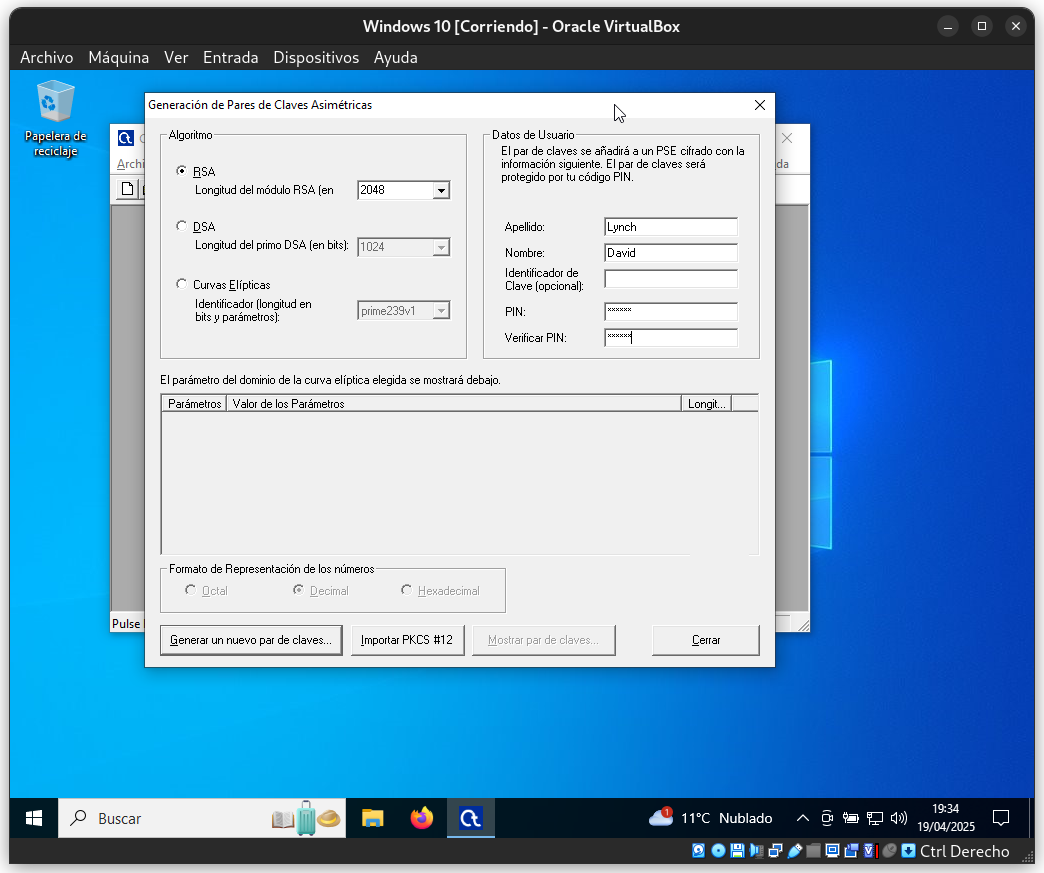
\includegraphics[width=\textwidth]{ClavesRSA-01.png}
    \caption{Generación del perfil del par de claves RSA}
\end{figure}

\begin{figure}[H]
    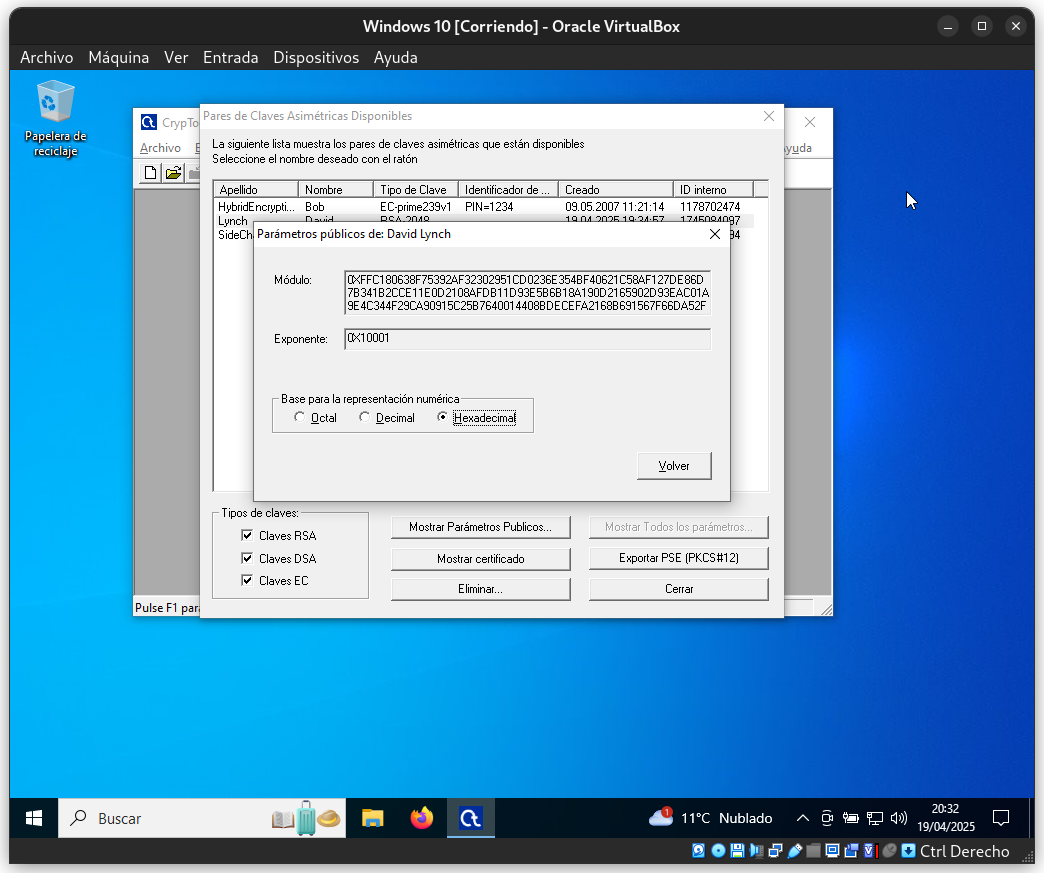
\includegraphics[width=\textwidth]{ClavesRSA-02.png}
    \caption{Parámetros públicos de la clave (n, e)}
\end{figure}

\begin{figure}[H]
    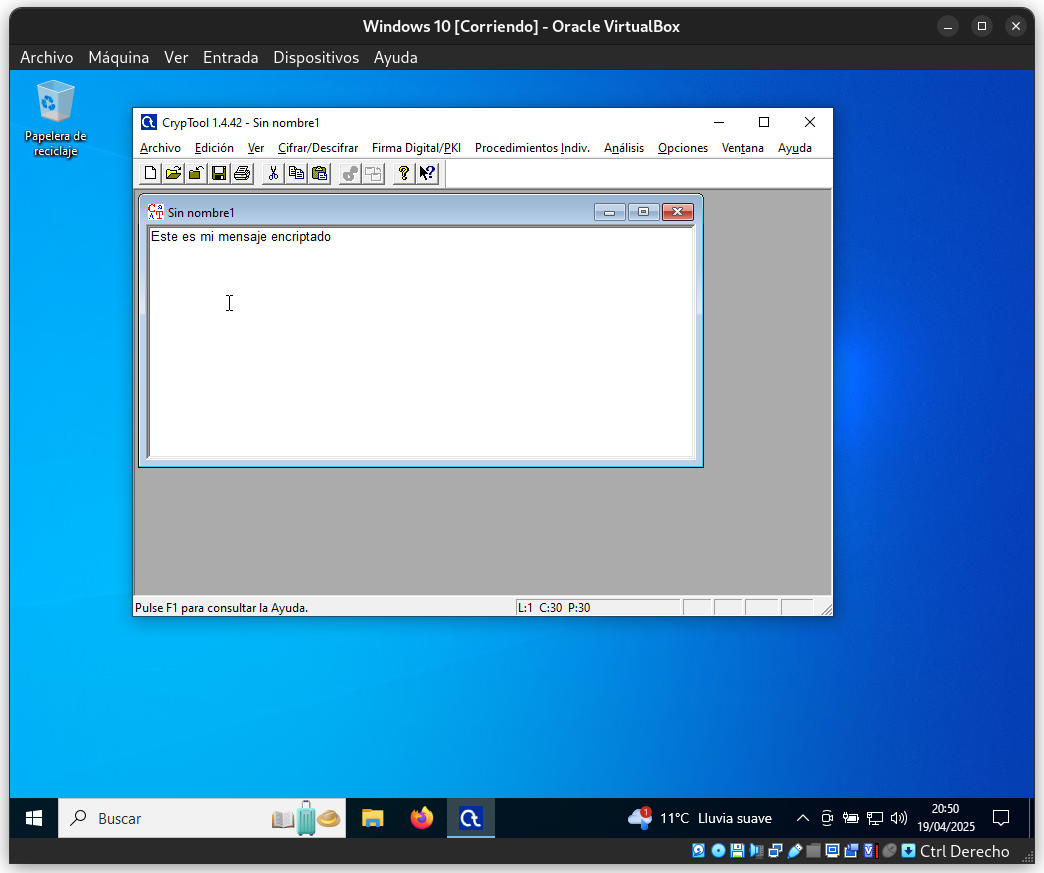
\includegraphics[width=\textwidth]{ClavesRSA-03.png}
    \caption{Pantalla del PIN de usuario}
\end{figure}

\begin{figure}[H]
    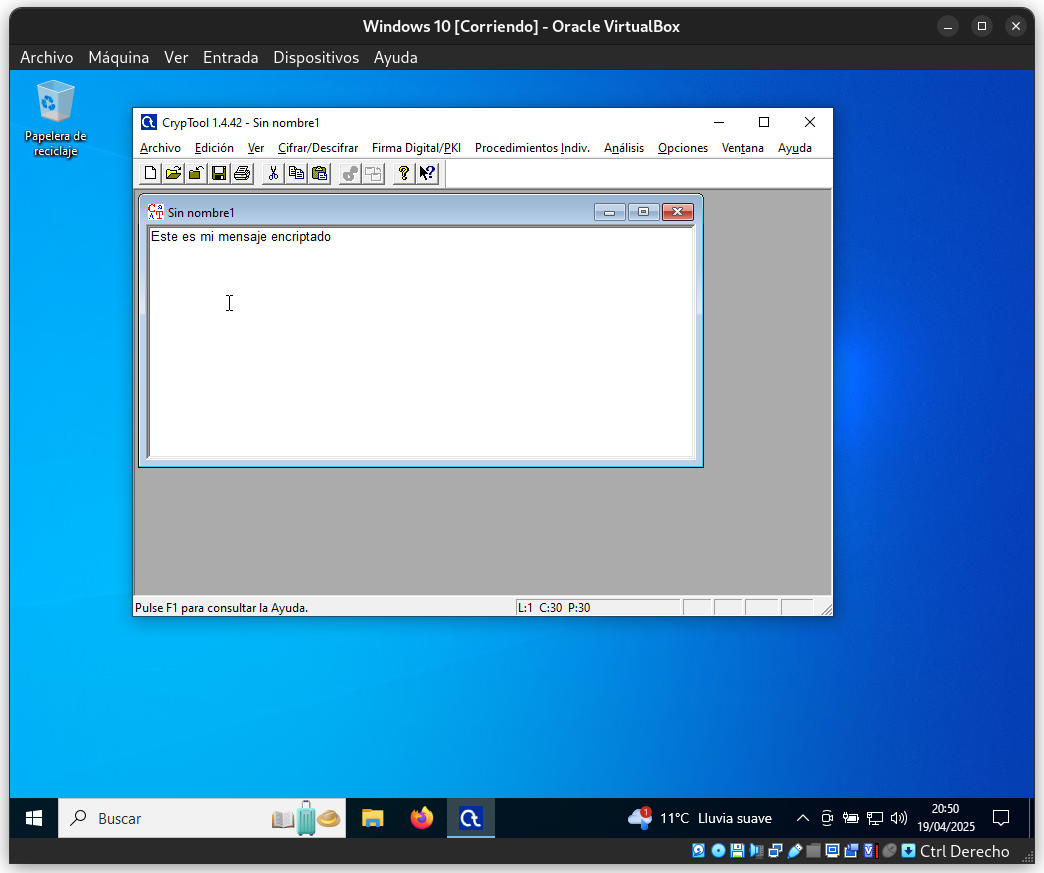
\includegraphics[width=\textwidth]{ClavesRSA-04.png}
    \caption{Texto de ejemplo para encriptar}
\end{figure}

\begin{figure}[H]
    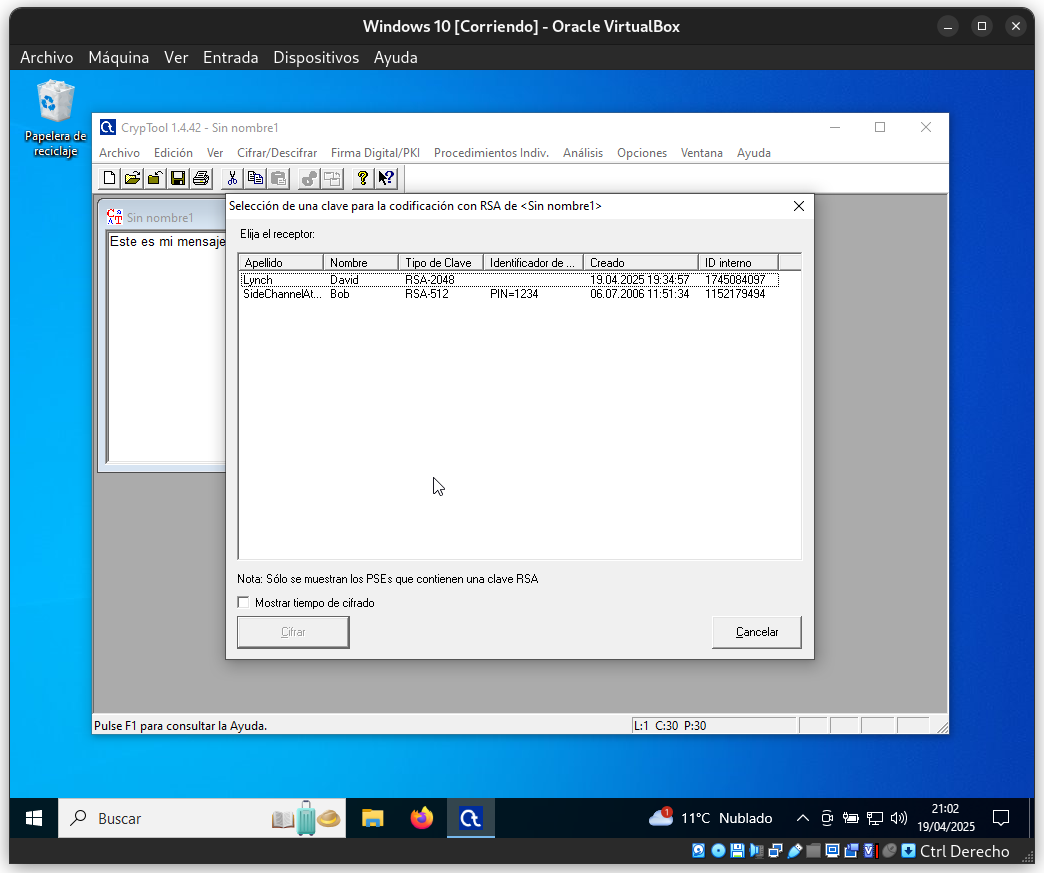
\includegraphics[width=\textwidth]{ClavesRSA-05.png}
    \caption{Generación del perfil del par de claves RSA}
\end{figure}

\begin{figure}[H]
    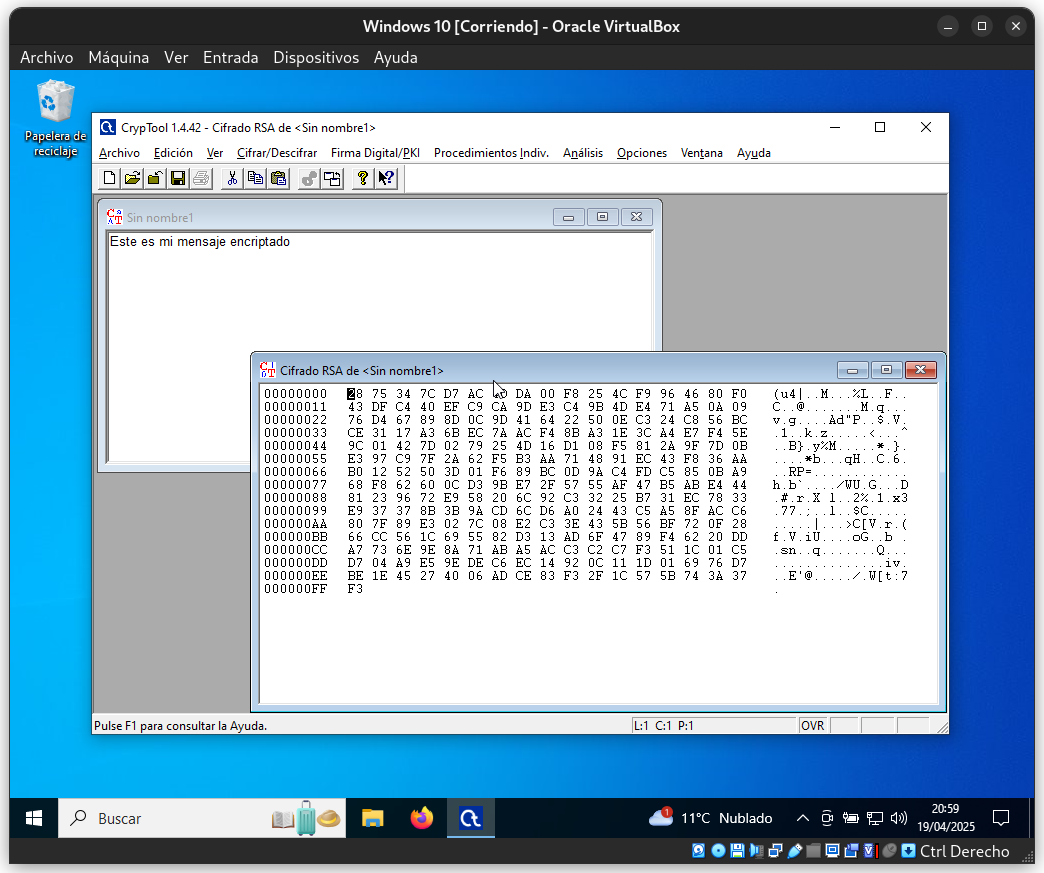
\includegraphics[width=\textwidth]{ClavesRSA-06.png}
    \caption{Generación del perfil del par de claves RSA}
\end{figure}

\begin{figure}[H]
    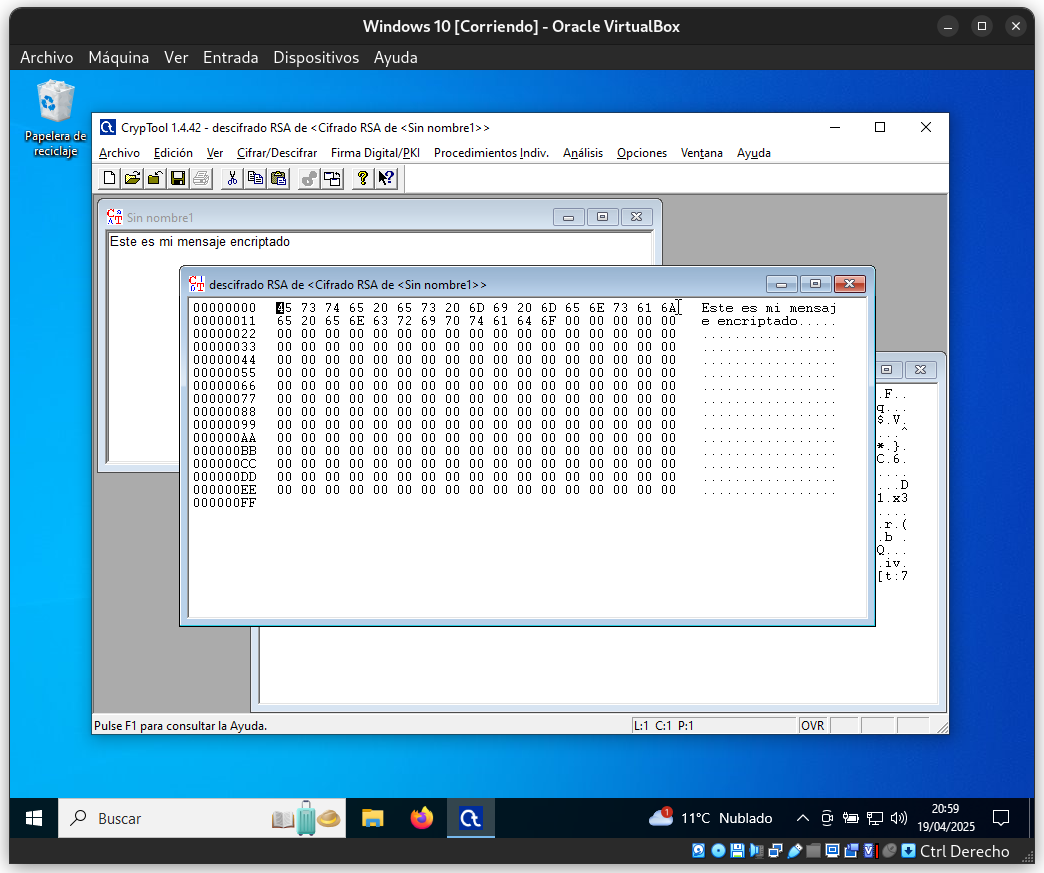
\includegraphics[width=\textwidth]{ClavesRSA-07.png}
    \caption{Generación del perfil del par de claves RSA}
\end{figure}


\subsubsection{¿Qué números conforman la clave pública?}

La clave pública está formada principalmente por dos números. El primero de ellos es el módulo ‘n’, que consiste en el producto de dos números primos (‘p’ y ‘q’ vistos en las clases teóricas) y es común tanto a la clave pública como a la privada. El segundo es el exponente público ‘e’, que suele tomar el valor de 65537. 

\subsubsection{¿A qué nos referimos con tamaño de clave?}

Como se explica en el apartado anterior, la clave está formada por dos números: ‘n’ y ‘e’. Que la clave tenga 2048 bits significa que el módulo ‘n’ tiene ese tamaño.  

Este tamaño nos indica la dificultad que tendría un ataque de fuerza bruta y el tamaño máximo a cifrar con esa clave. 


\subsubsection{Pruebas cifrado y descifrado}

\begin{figure}[H]
    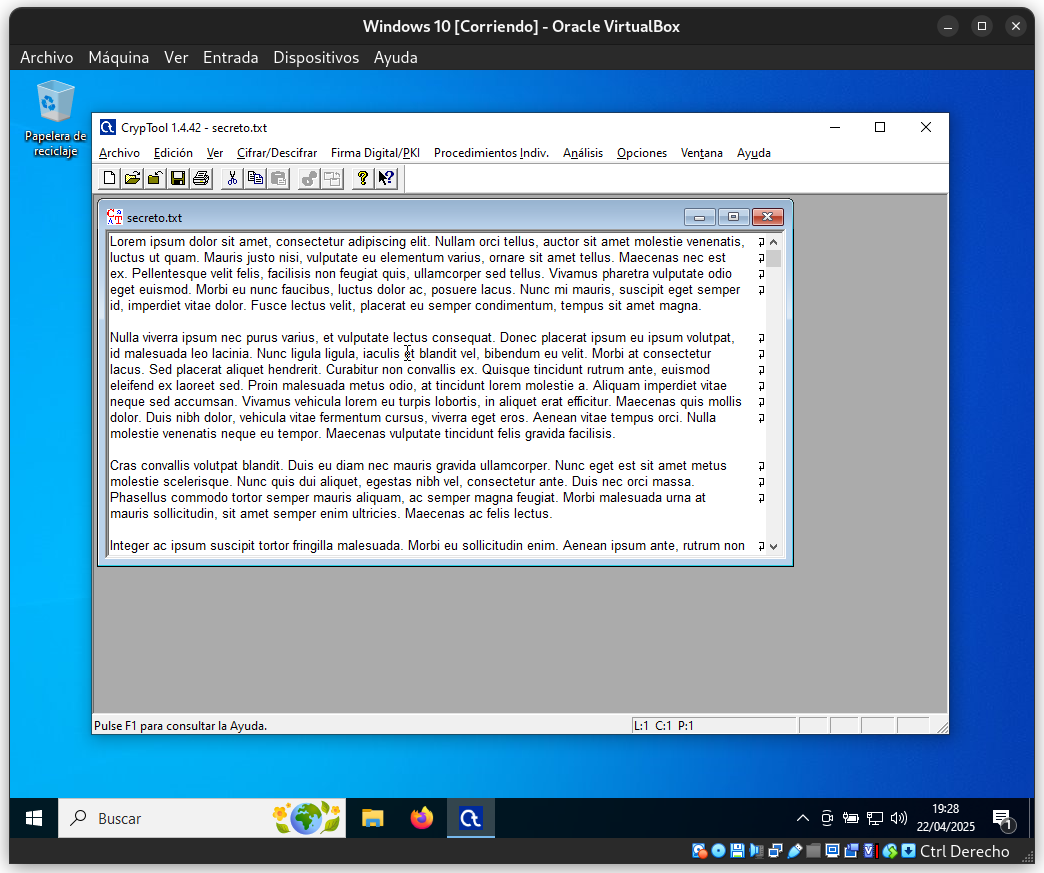
\includegraphics[width=\textwidth]{EncriptadoRSA-1}
    \caption{Generación del perfil del par de claves RSA}
\end{figure}

\begin{figure}[H]
    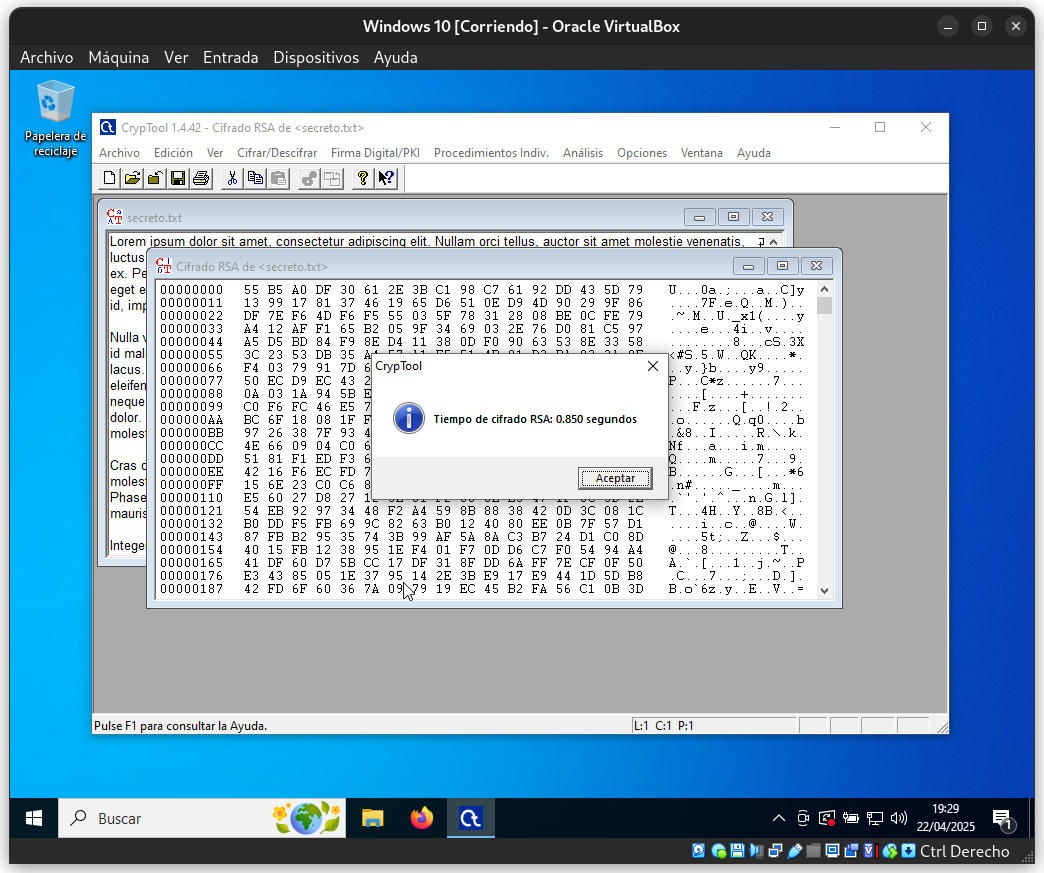
\includegraphics[width=\textwidth]{EncriptadoRSA-2}
    \caption{Generación del perfil del par de claves RSA}
\end{figure}

\begin{figure}[H]
    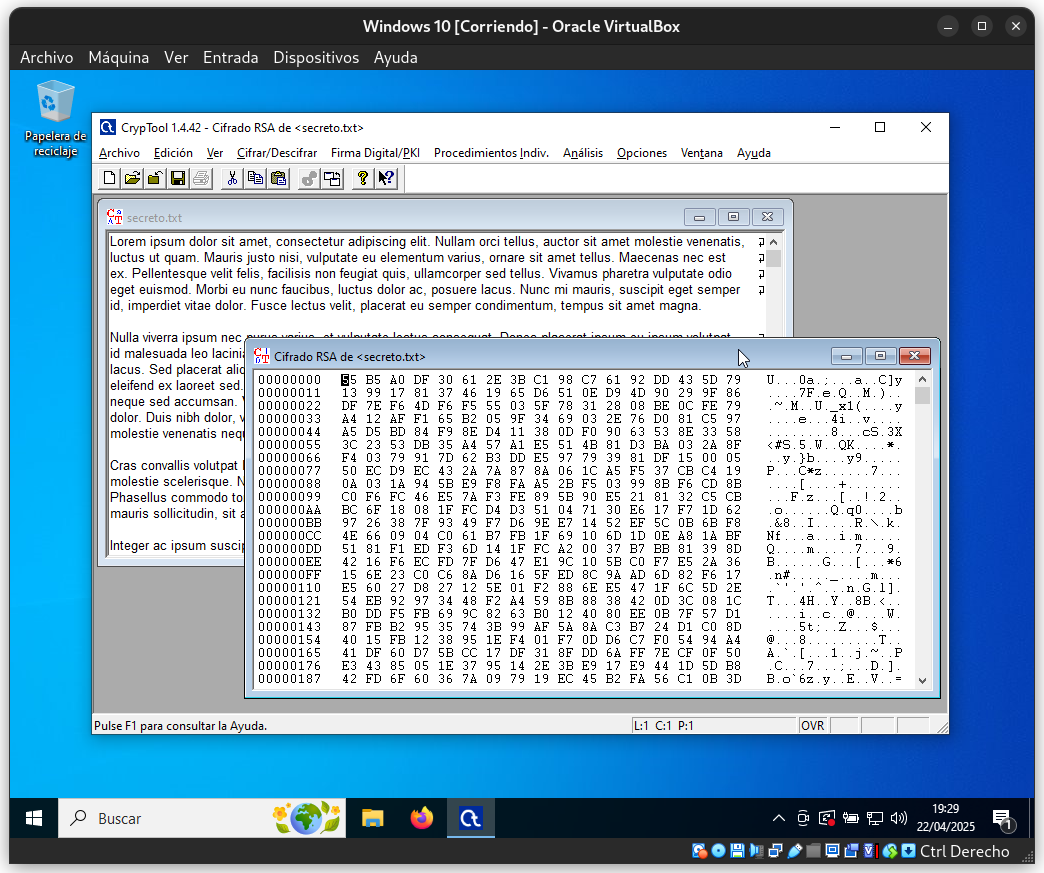
\includegraphics[width=\textwidth]{EncriptadoRSA-3}
    \caption{Generación del perfil del par de claves RSA}
\end{figure}

\begin{figure}[H]
    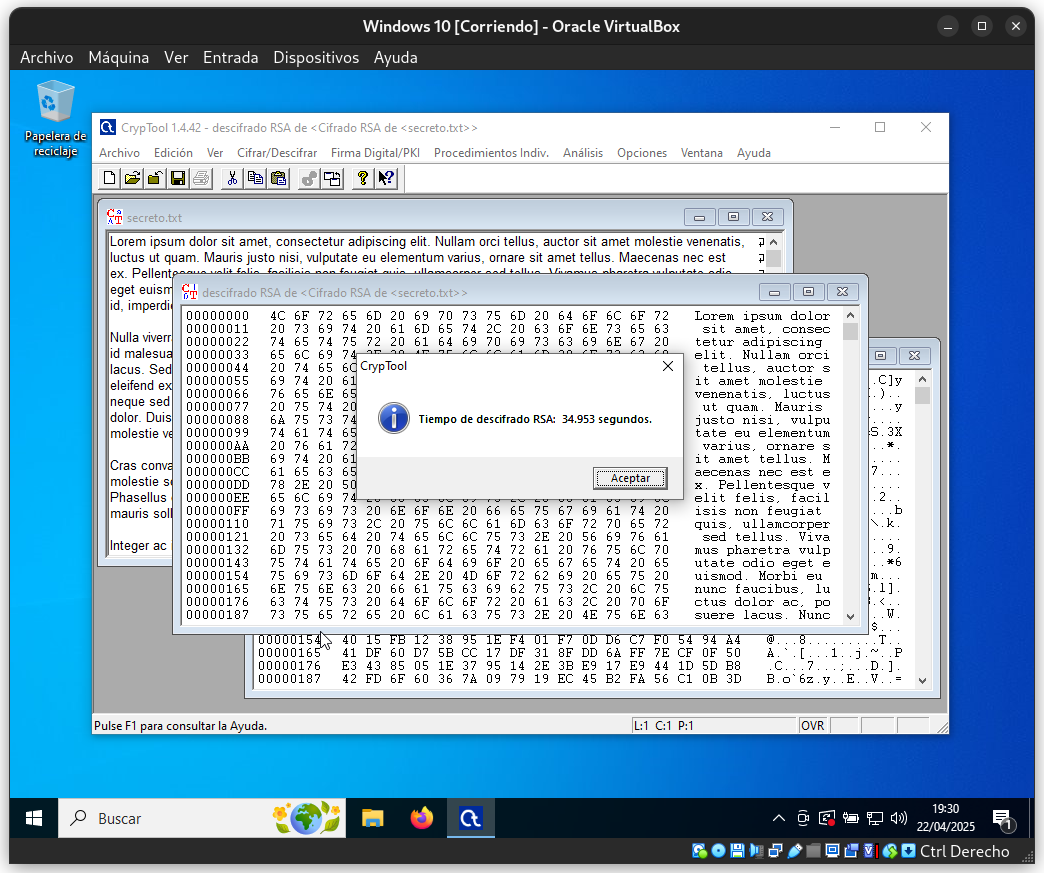
\includegraphics[width=\textwidth]{DesencriptadoRSA-1}
    \caption{Generación del perfil del par de claves RSA}
\end{figure}

\begin{figure}[H]
    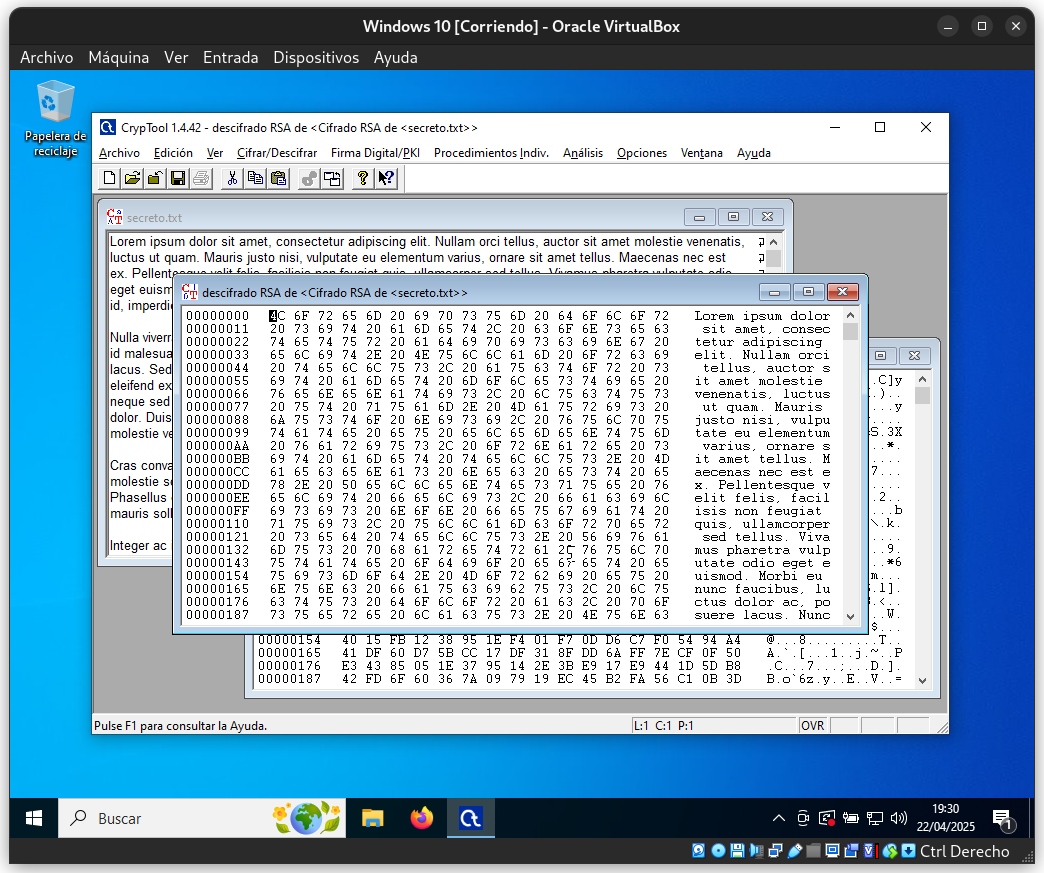
\includegraphics[width=\textwidth]{DesencriptadoRSA-2}
    \caption{Generación del perfil del par de claves RSA}
\end{figure}

\subsection{Ejercicio 2}
\graphicspath{ {img/02} }

\subsubsection{Generación claves RSA OpenSSL}

\begin{figure}[H]   
    \centering
    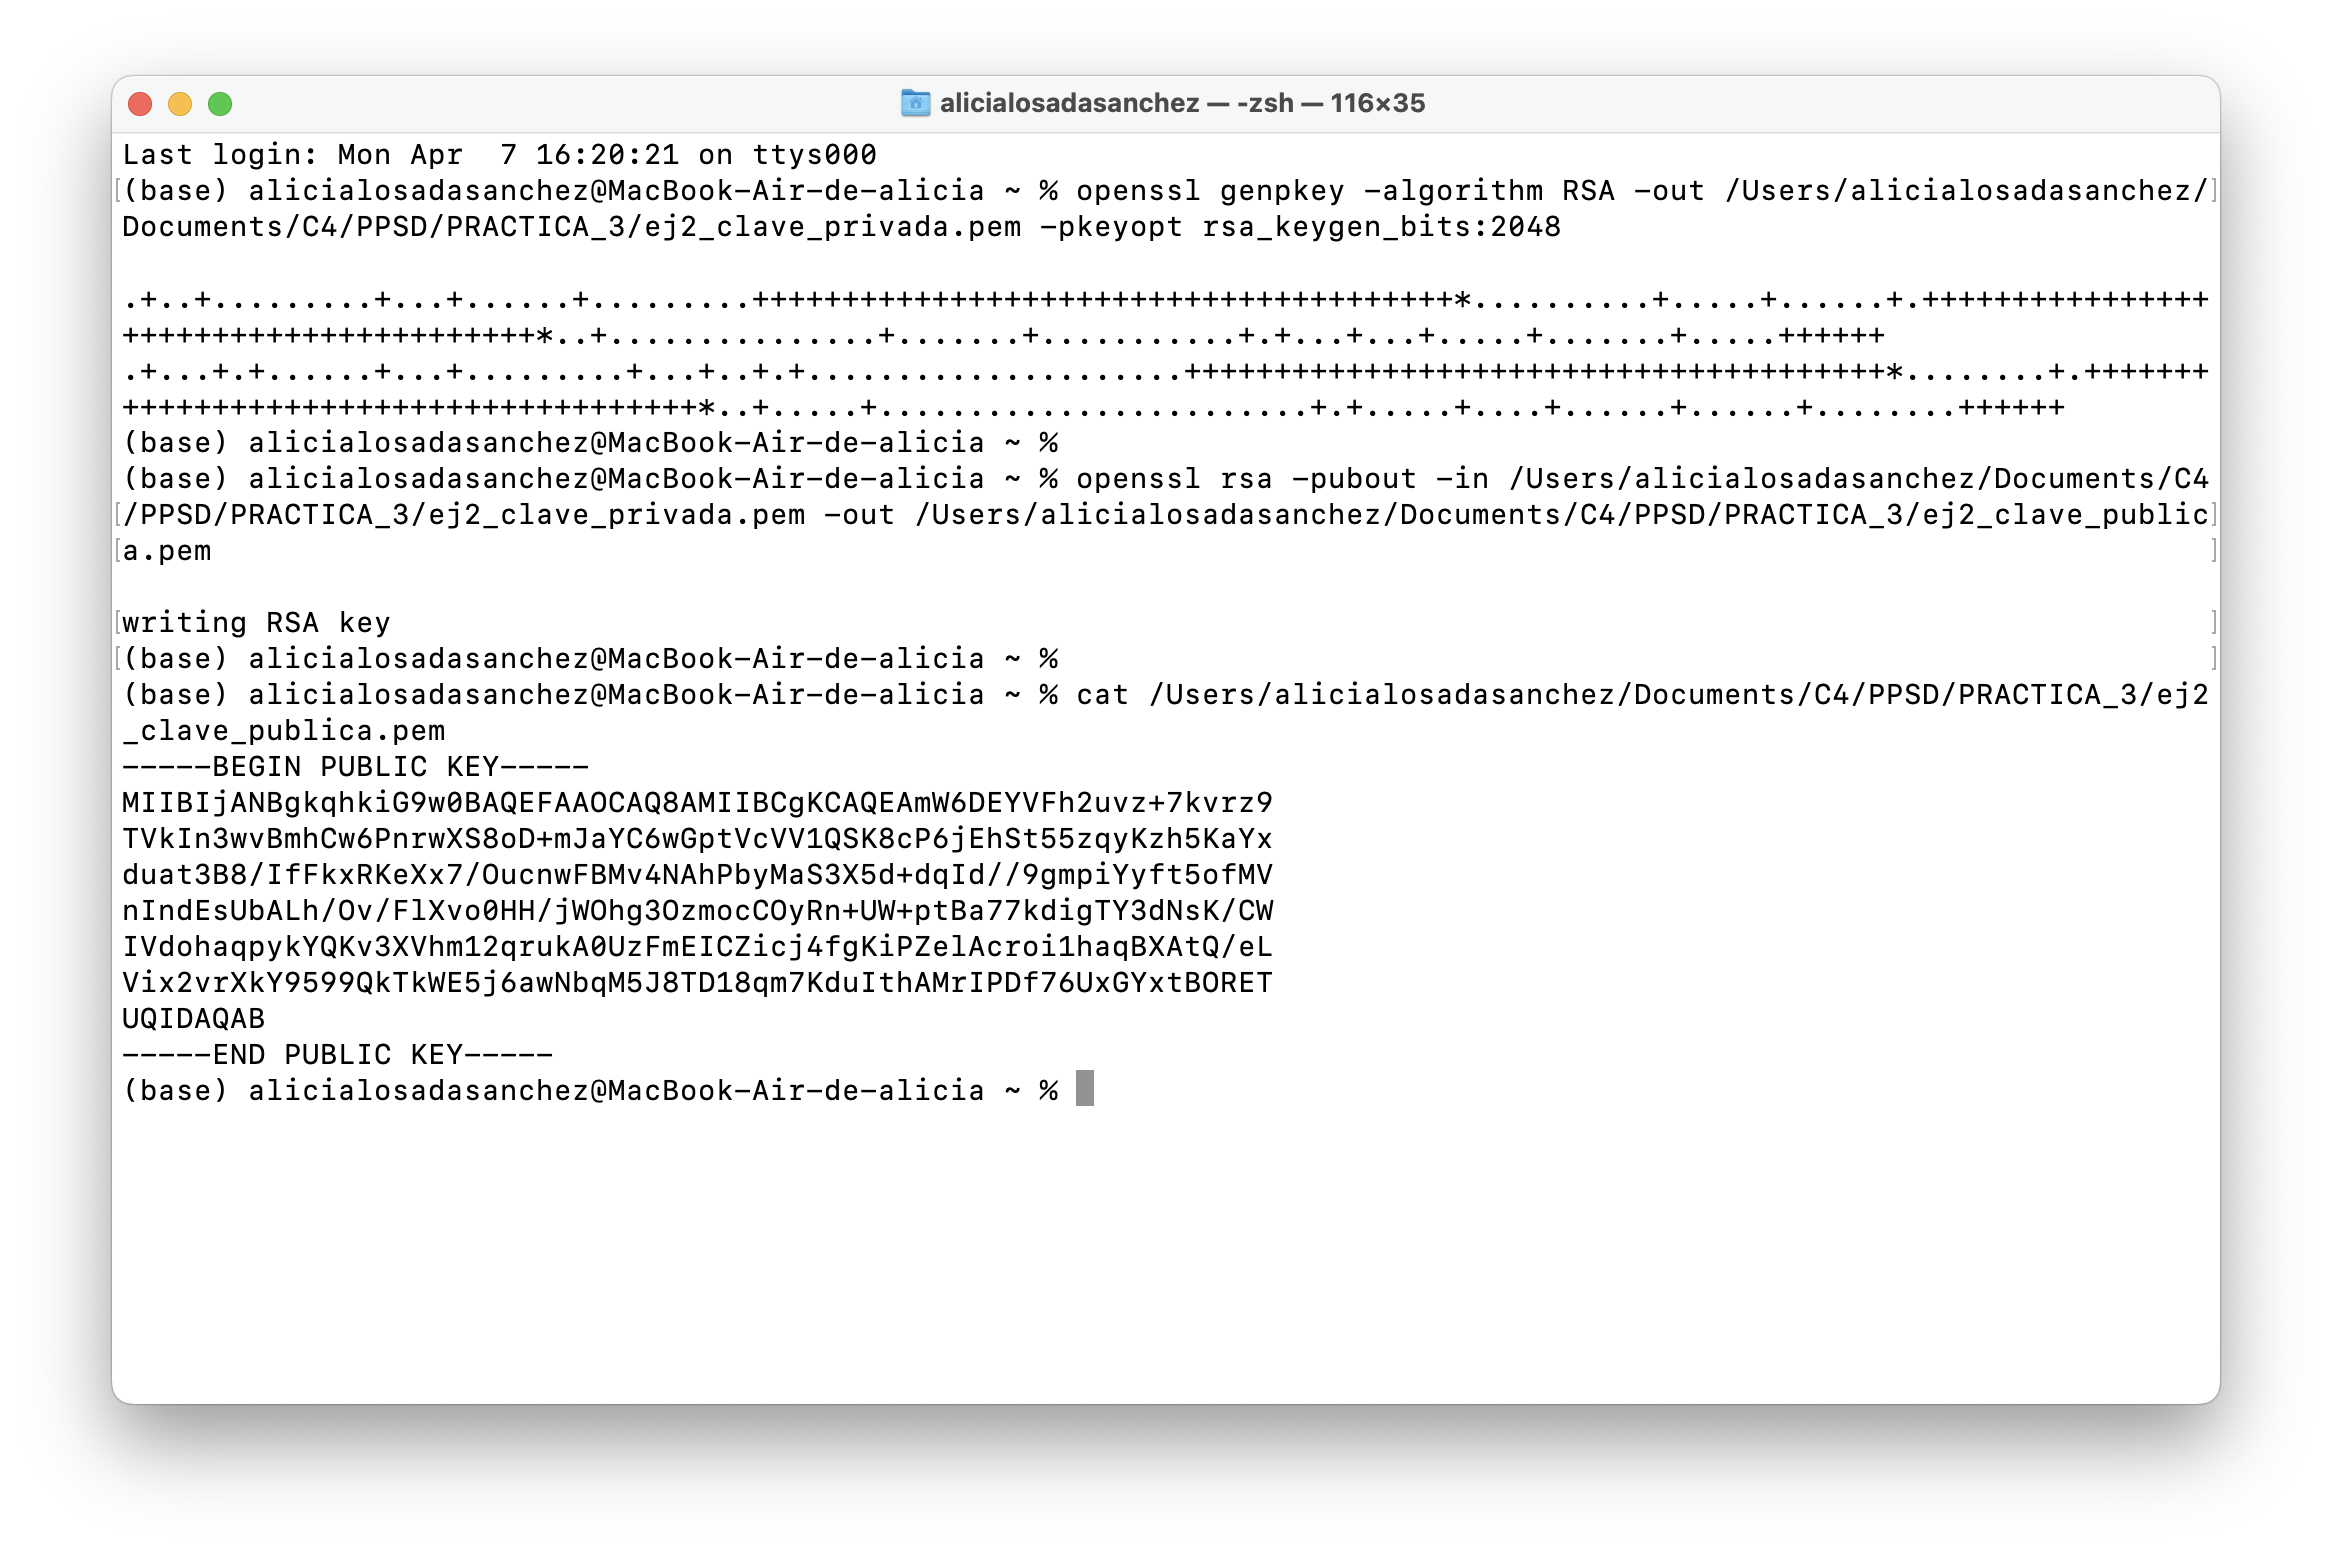
\includegraphics[width=\textwidth]{ej2_a.png}
    \caption{Generación clave RSA OpenSSL}
    \label{fig:generacion_rsa_openssl}
\end{figure}

Con el primer comando de la \ref{fig:generacion_rsa_openssl} generamos una clave privada de 2048 bits. Obtenemos la clave pública desde la clave privada con el segundo comando. En la \ref{fig:generacion_rsa_openssl} se puede ver el contenido de la clave pública. 


\subsubsection{¿Qué números conforman la clave pública?}

\begin{figure}[H]   
    \centering
    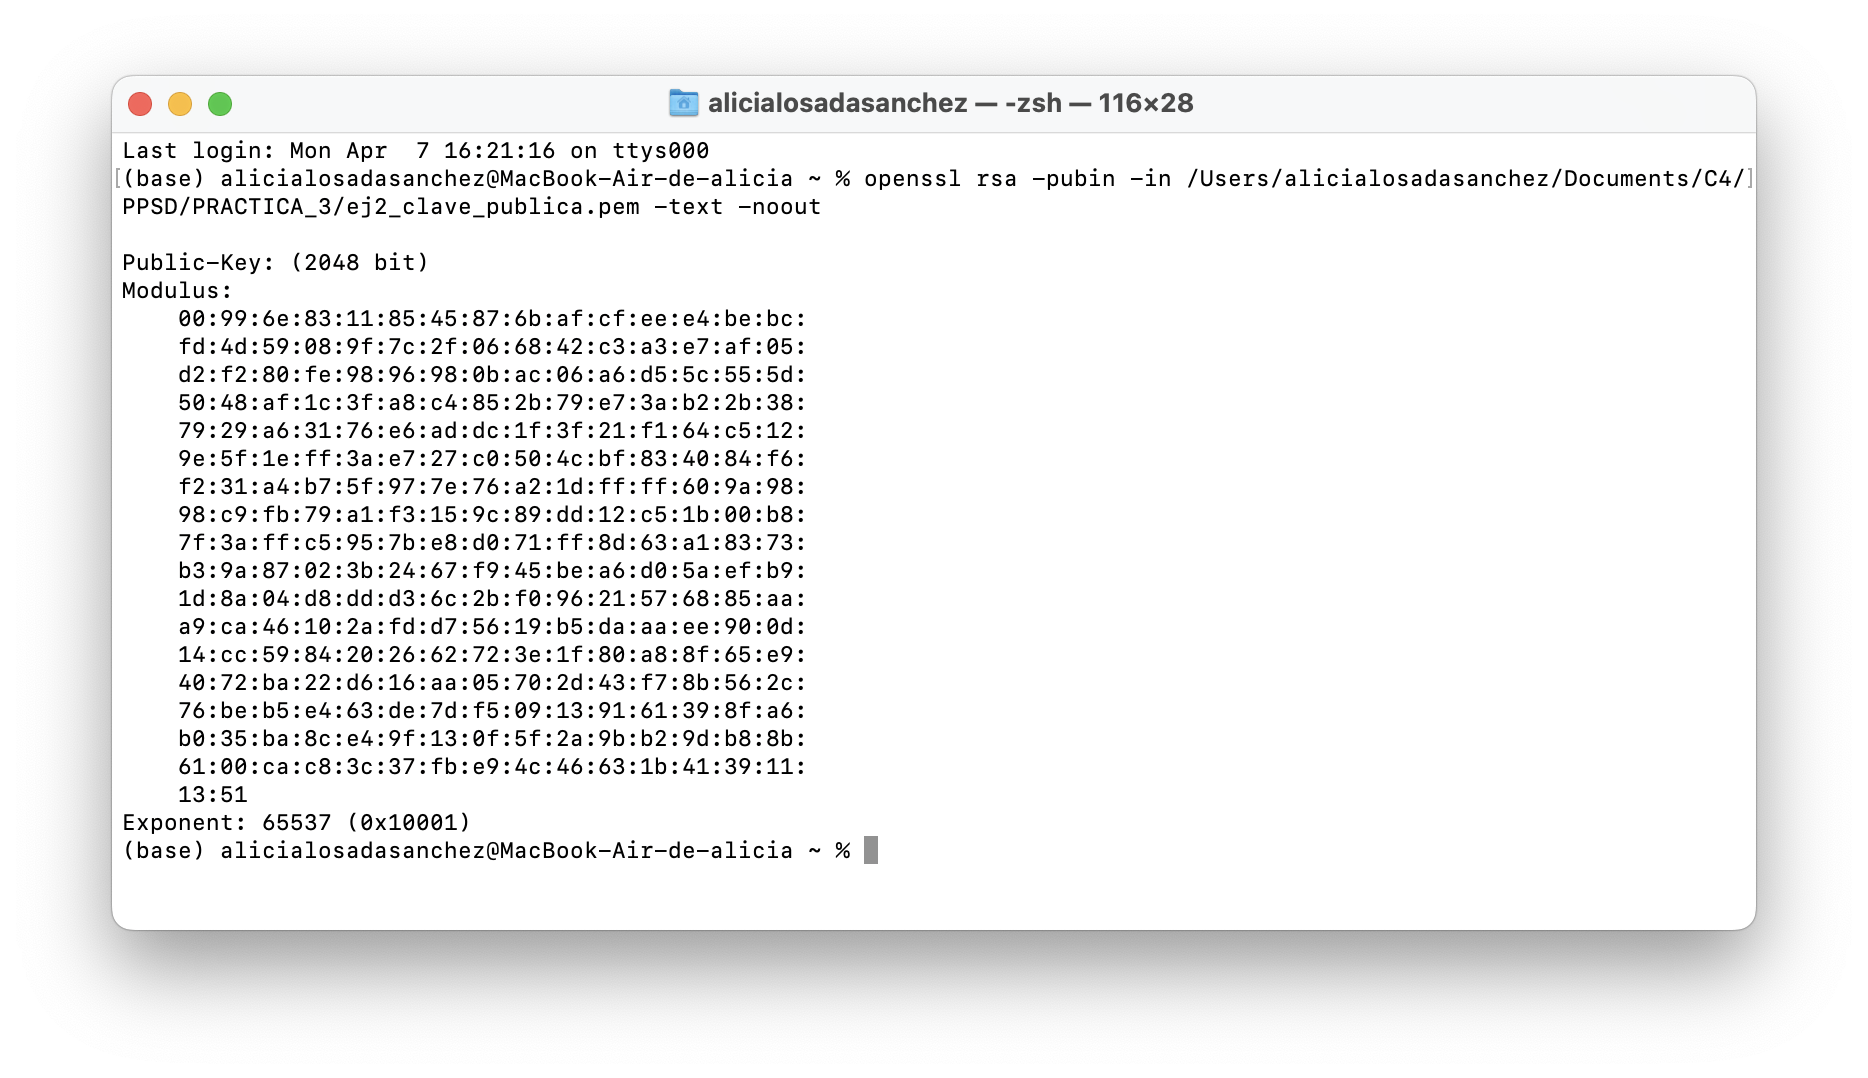
\includegraphics[width=\textwidth]{ej2_b.png}
    \caption{Partes clave pública}
    \label{fig:partes_clave_publica_rsa_openssl}
\end{figure}

Como se explica en el ejercicio 1, la clave pública está formada principalmente por dos números. El primero de ellos es el módulo ‘n’, que consiste en el producto de dos números primos (p y q vistos en las clases teóricas) y es común tanto a la clave pública como a la privada. El segundo es el exponente público ‘e’ que, como sucede en este caso, suele tomar el valor de 65537. En la \ref{fig:partes_clave_publica_rsa_openssl} se ve cuáles son esos valores para la clave previamente creada. 

\subsubsection{Cifrado secreto}

\begin{figure}[H]   
    \centering
    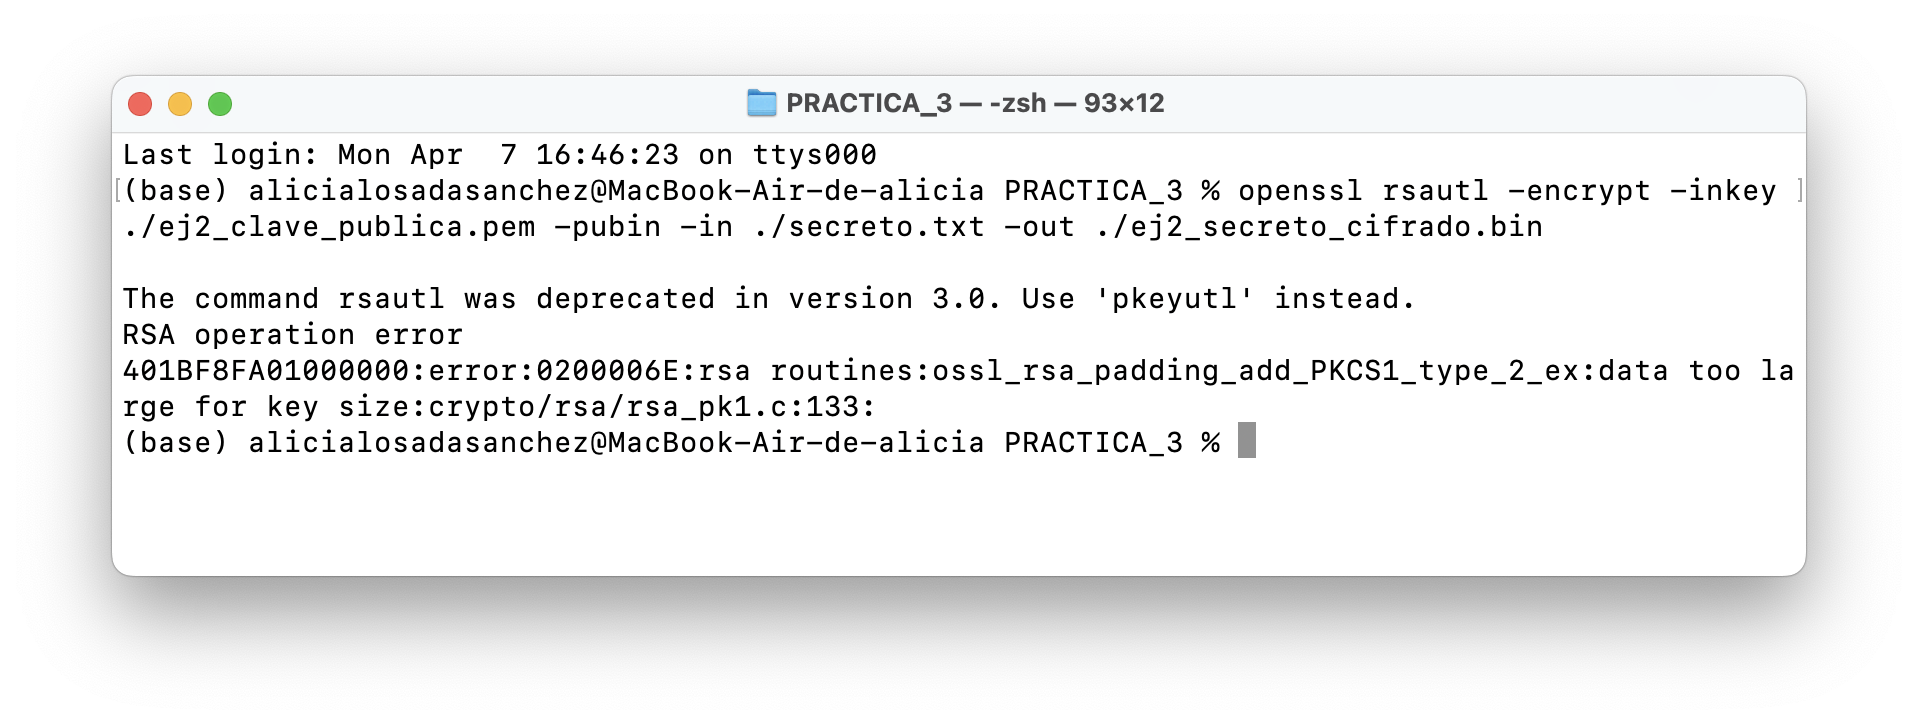
\includegraphics[width=\textwidth]{ej2_c.png}
    \caption{Cifrado secreto.txt}
    \label{fig:cifrado_secreto_openssl}
\end{figure}

El comando para cifrar el archivo secreto.txt con la clave pública generada se ve en la \ref{fig:cifrado_secreto_openssl}. Como se ve, obtuvimos una limitación al ejecutar el comando debido a que el tamaño del archivo.  

RSA es un algoritmo de cifrado asimétrico, diseñado para trabajar con bloques de datos pequeños. El archivo secreto.txt contiene más de 5000 caracteres, por lo que no es posible cifrarlo directamente con RSA. 

La solución que proponemos es llevar a cabo un cifrado mixto o híbrido, es decir, utilizar dos algoritmos de cifrado, uno simétrico y otro asimétrico. AES es un algoritmo de cifrado simétrico de bloques que permite el uso de claves de hasta 256 bits. 

Nuestra propuesta consiste en cifrar nuestro archivo secreto.txt con AES usando una clave secreta de 256 bits. Posteriormente, esta clave será la que se cifrará usando RSA, ya que sí cabe dentro del límite del algoritmo. 

\subsection{Ejercicio 3}
\graphicspath{ {img/03} }

\subsubsection{Generación clave D\&H}

COMPLETAR

\subsubsection{Utilidad clave}

La clave generada mediante el protocolo D\&H (Diffie-Hellman) se usa para establecer un secreto compartido entre dos usuarios, incluso si se comunican a través de un canal inseguro como Internet. Este secreto compartido puede servir, por ejemplo, como clave simétrica para cifrar y descifrar mensajes. 

La funcionalidad de D\&H no es el cifrado de mensajes, sino permitir a las dos partes acordar una clave secreta. 

\subsubsection{Problemas de seguridad}

A pesar de parecer ser un método inteligente para el acuerdo de una clave secreta, si no se toman las medidas de seguridad necesarias, puede llegar a ser un método vulnerable.  

Consideramos que el principal problema con el que nos podemos encontrar es que, como D\&H no autentica las partes participantes, un atacante puede interceptar los valores públicos y establecer claves falsas con ambas partes. Así, el atacante podrá leer y modificar los mensajes sin ser detectado. 

Esto se puede solucionar utilizando distintos tipos de métodos de autenticación, como certificado digital o firma digital, para verificar las identidades participantes. 

Por otra parte, si usamos parámetros débiles como un ‘p’ muy pequeño, como es nuestro caso, se hace posible un ataque por fuerza bruta o logaritmo discreto usando computadoras modernas. 

Esto se puede evitar haciendo uso de claves suficientemente grandes, así como valores seguros de ‘p’ y de ‘g’. 


\section{Certificados digitales}
\subsection{Ejercicio 4}
\graphicspath{ {img/04} }

\subsubsection{Certificados web}

Los sitios web seleccionados fueron:
\begin{itemize}
    \item \href{https://www.coruna.gal}{coruna.gal}
    \item \href{https://delthia.com}{delthia.com}
    \item \href{https://nap.transportes.gob.es}{nap.transportes.gob.es}
    \item \href{https://www.udc.es}{udc.es}
    \item \href{www.wikipedia.org}{wikipedia.org}
\end{itemize}

\begin{figure}[H]   
    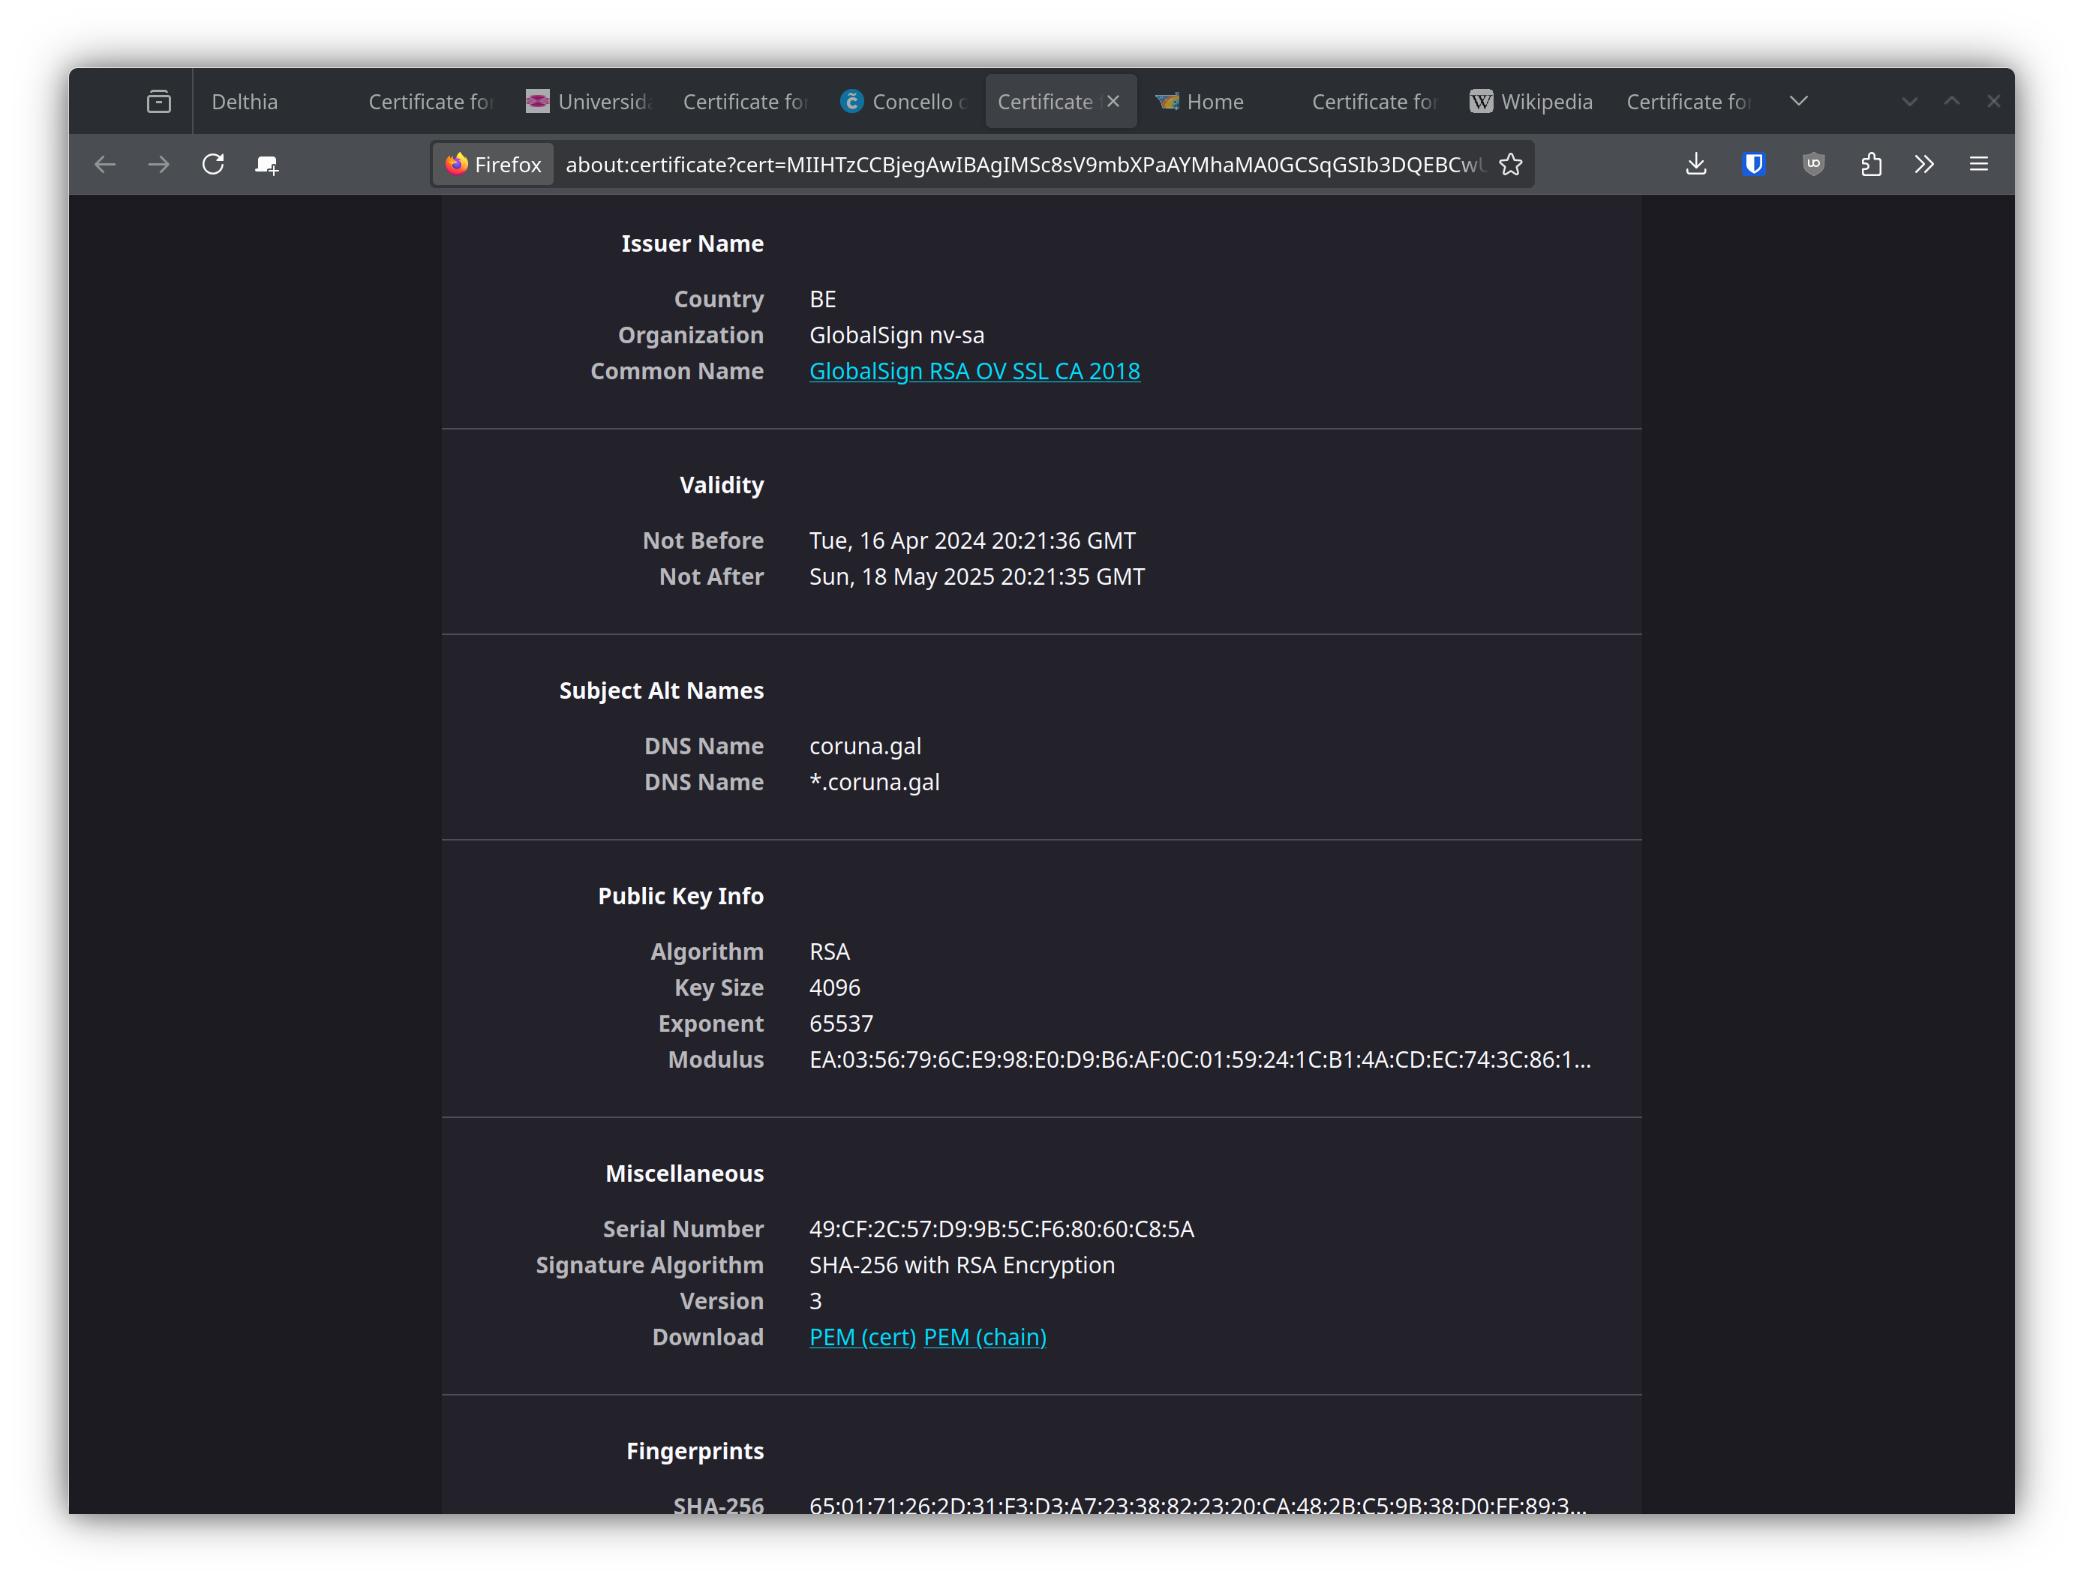
\includegraphics[width=15cm]{cert-coruna.png}
    \caption{Certificado de \url{coruna.gal}}
\end{figure}

\begin{figure}[H]
    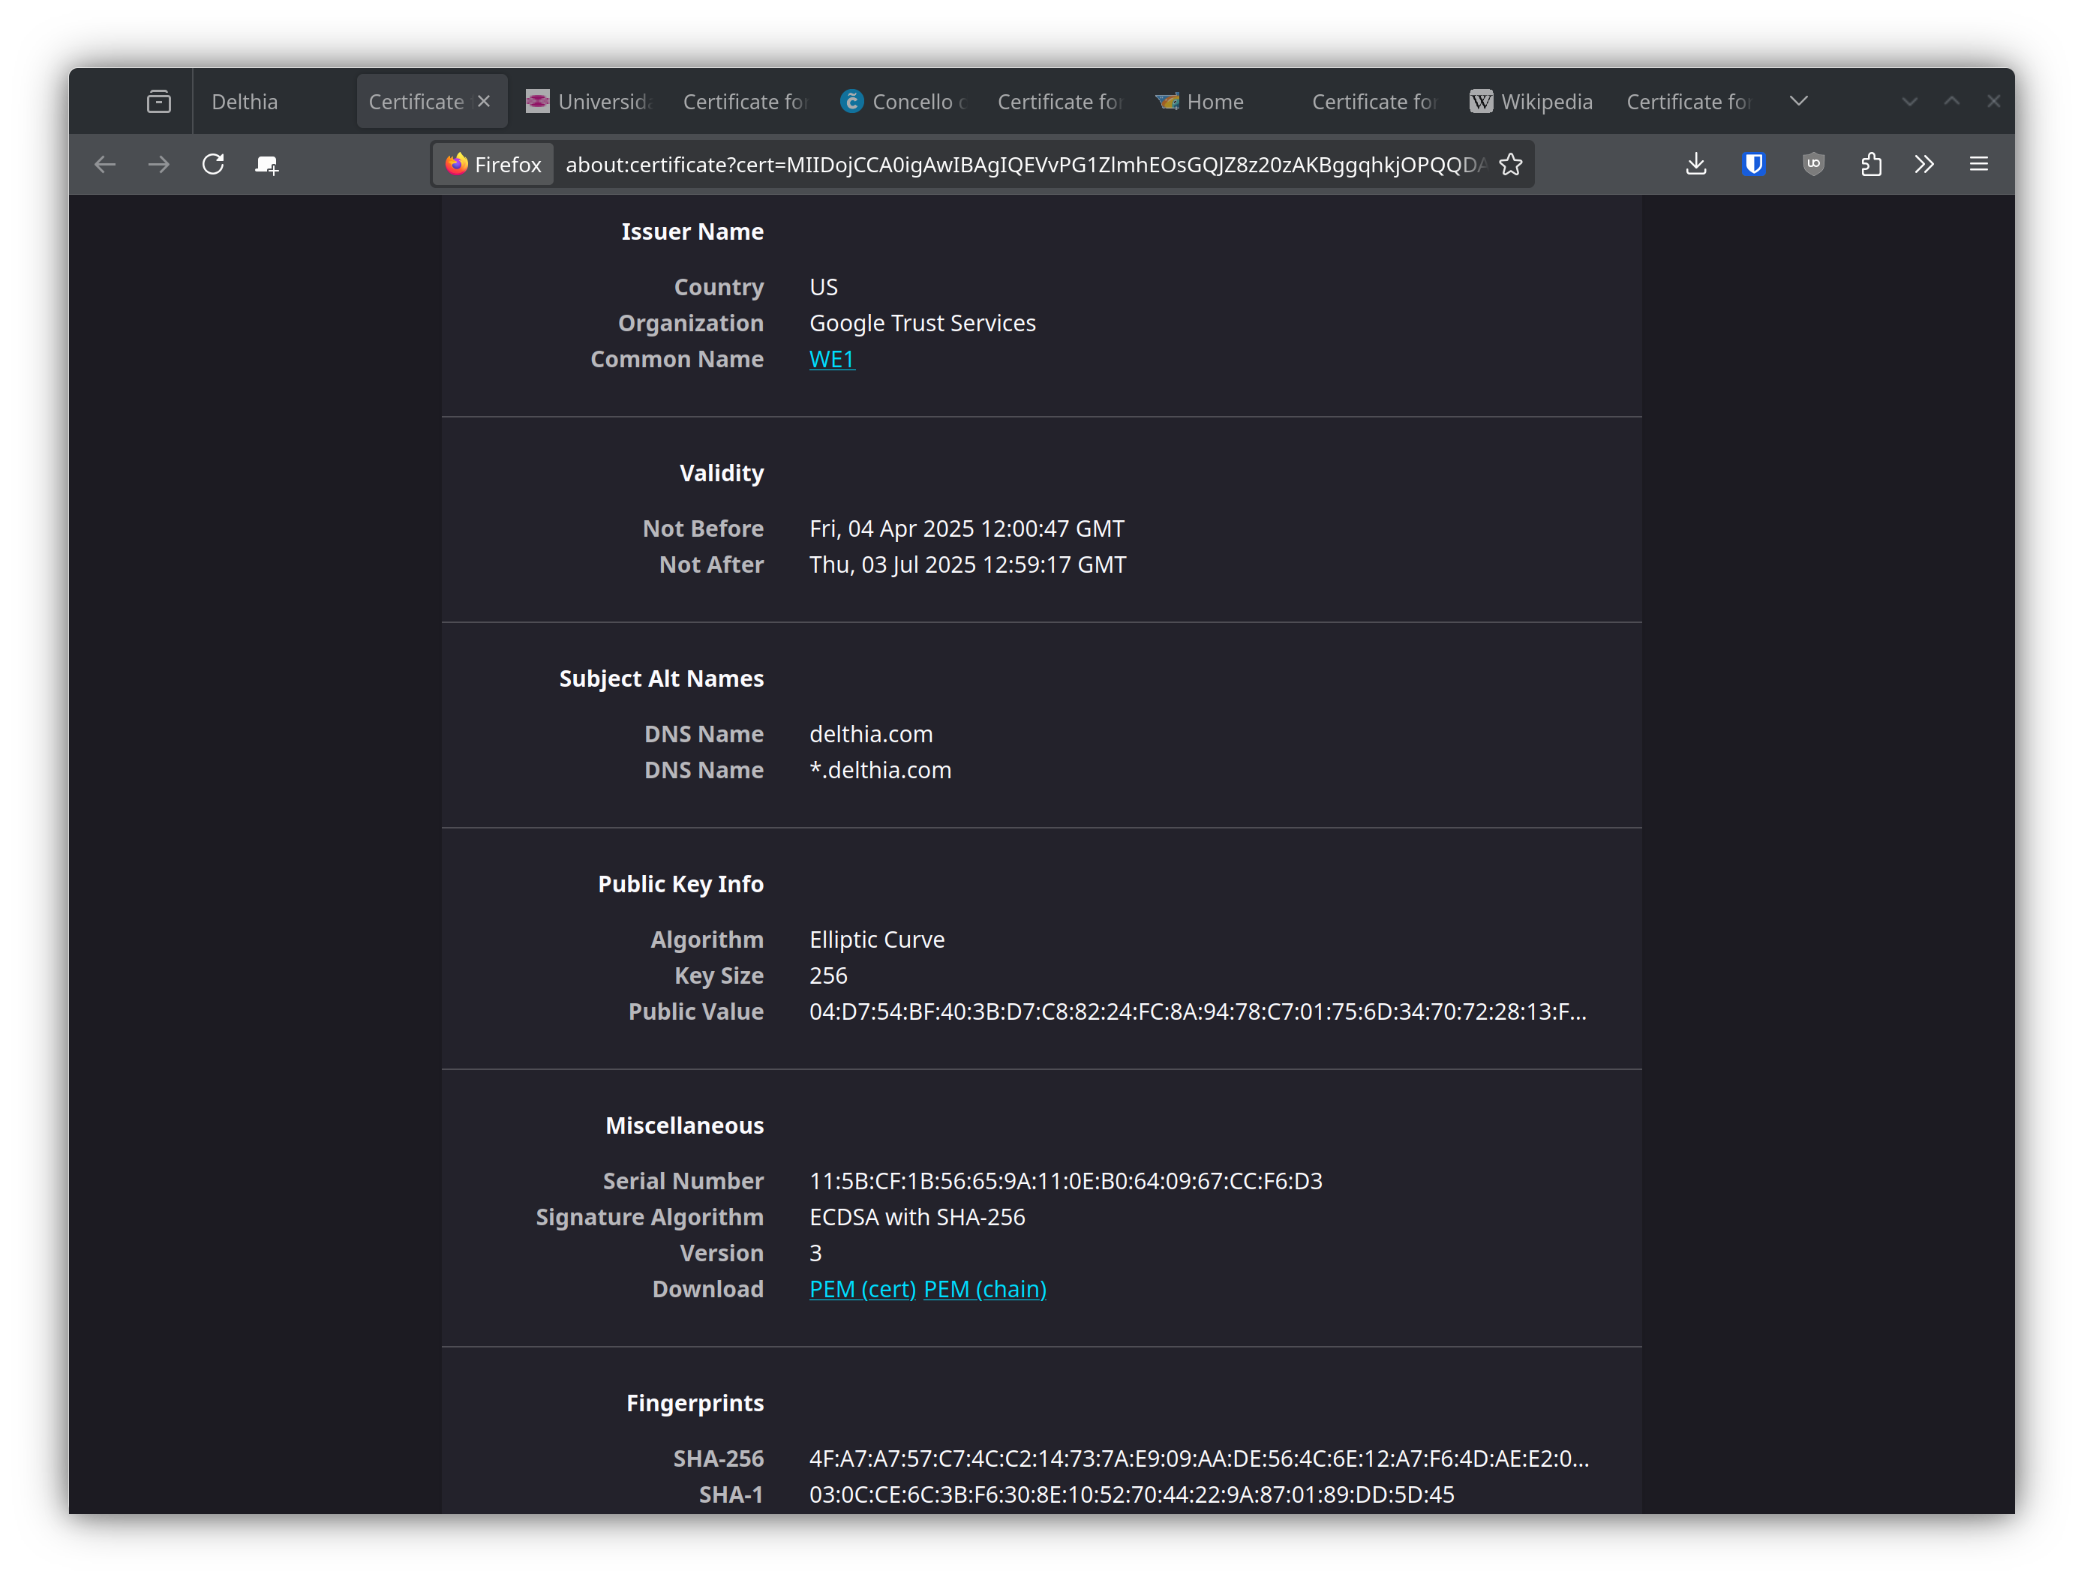
\includegraphics[width=15cm]{cert-delthia.png}
    \caption{Certificado de \url{delthia.com}}
\end{figure}

\begin{figure}[H]
    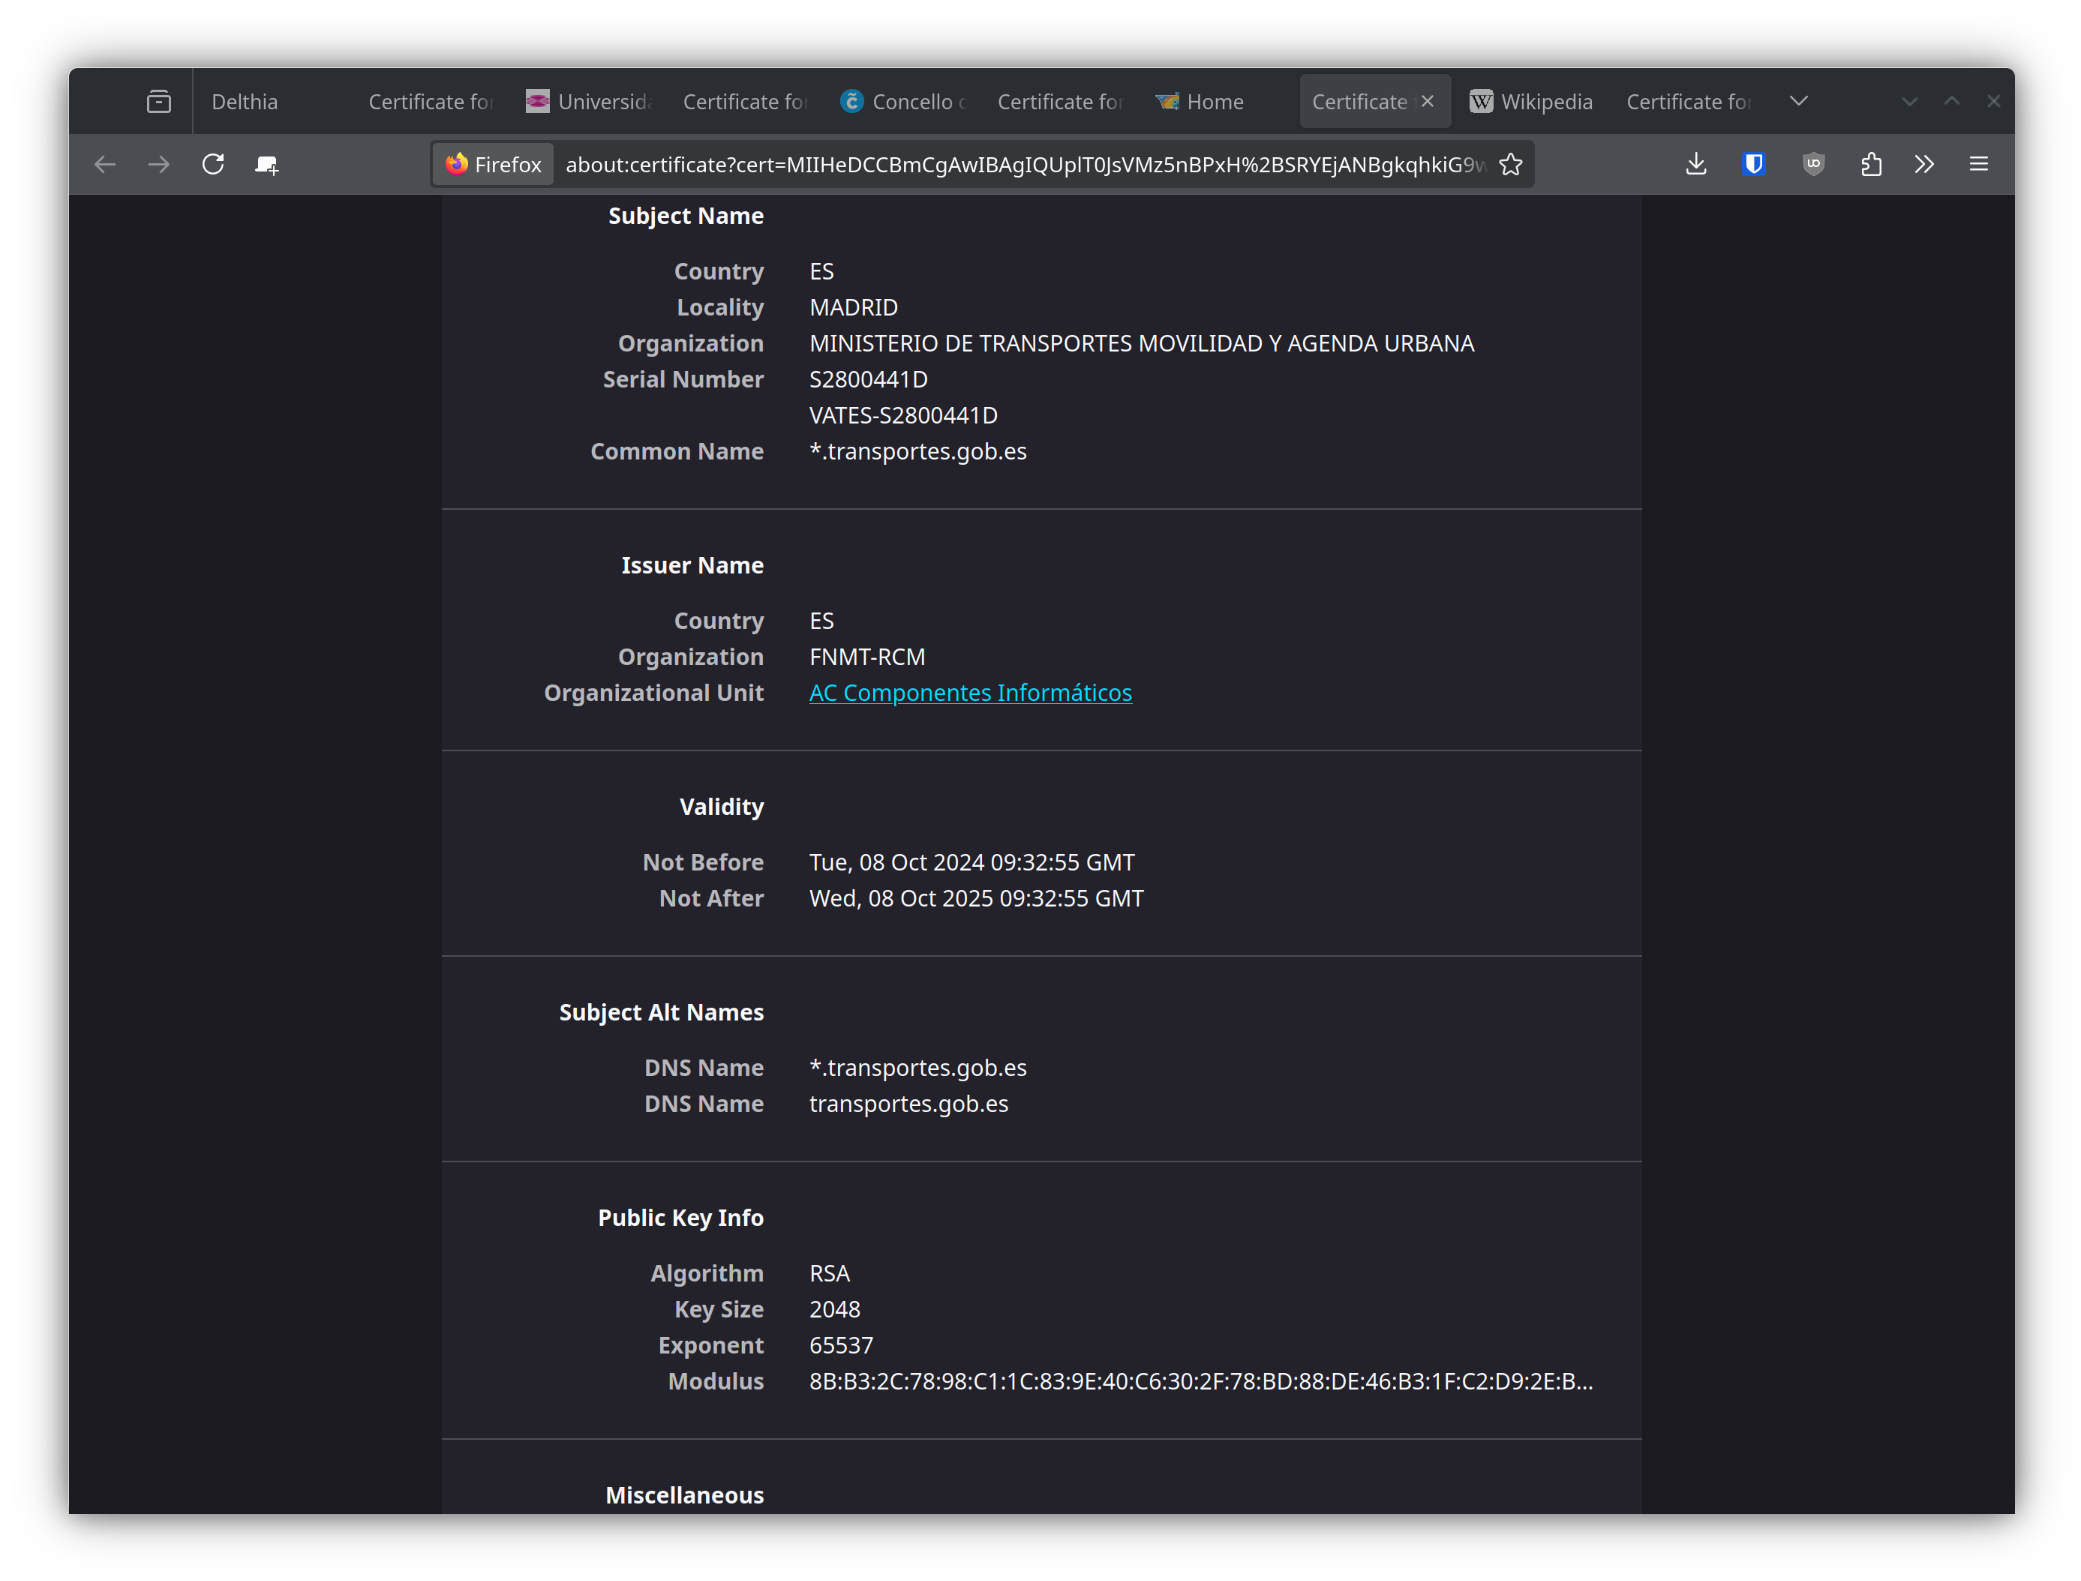
\includegraphics[width=15cm]{cert-transportes.png}
    \caption{Certificado de \url{nap.transportes.gob.es}}
\end{figure}

\begin{figure}[H]
    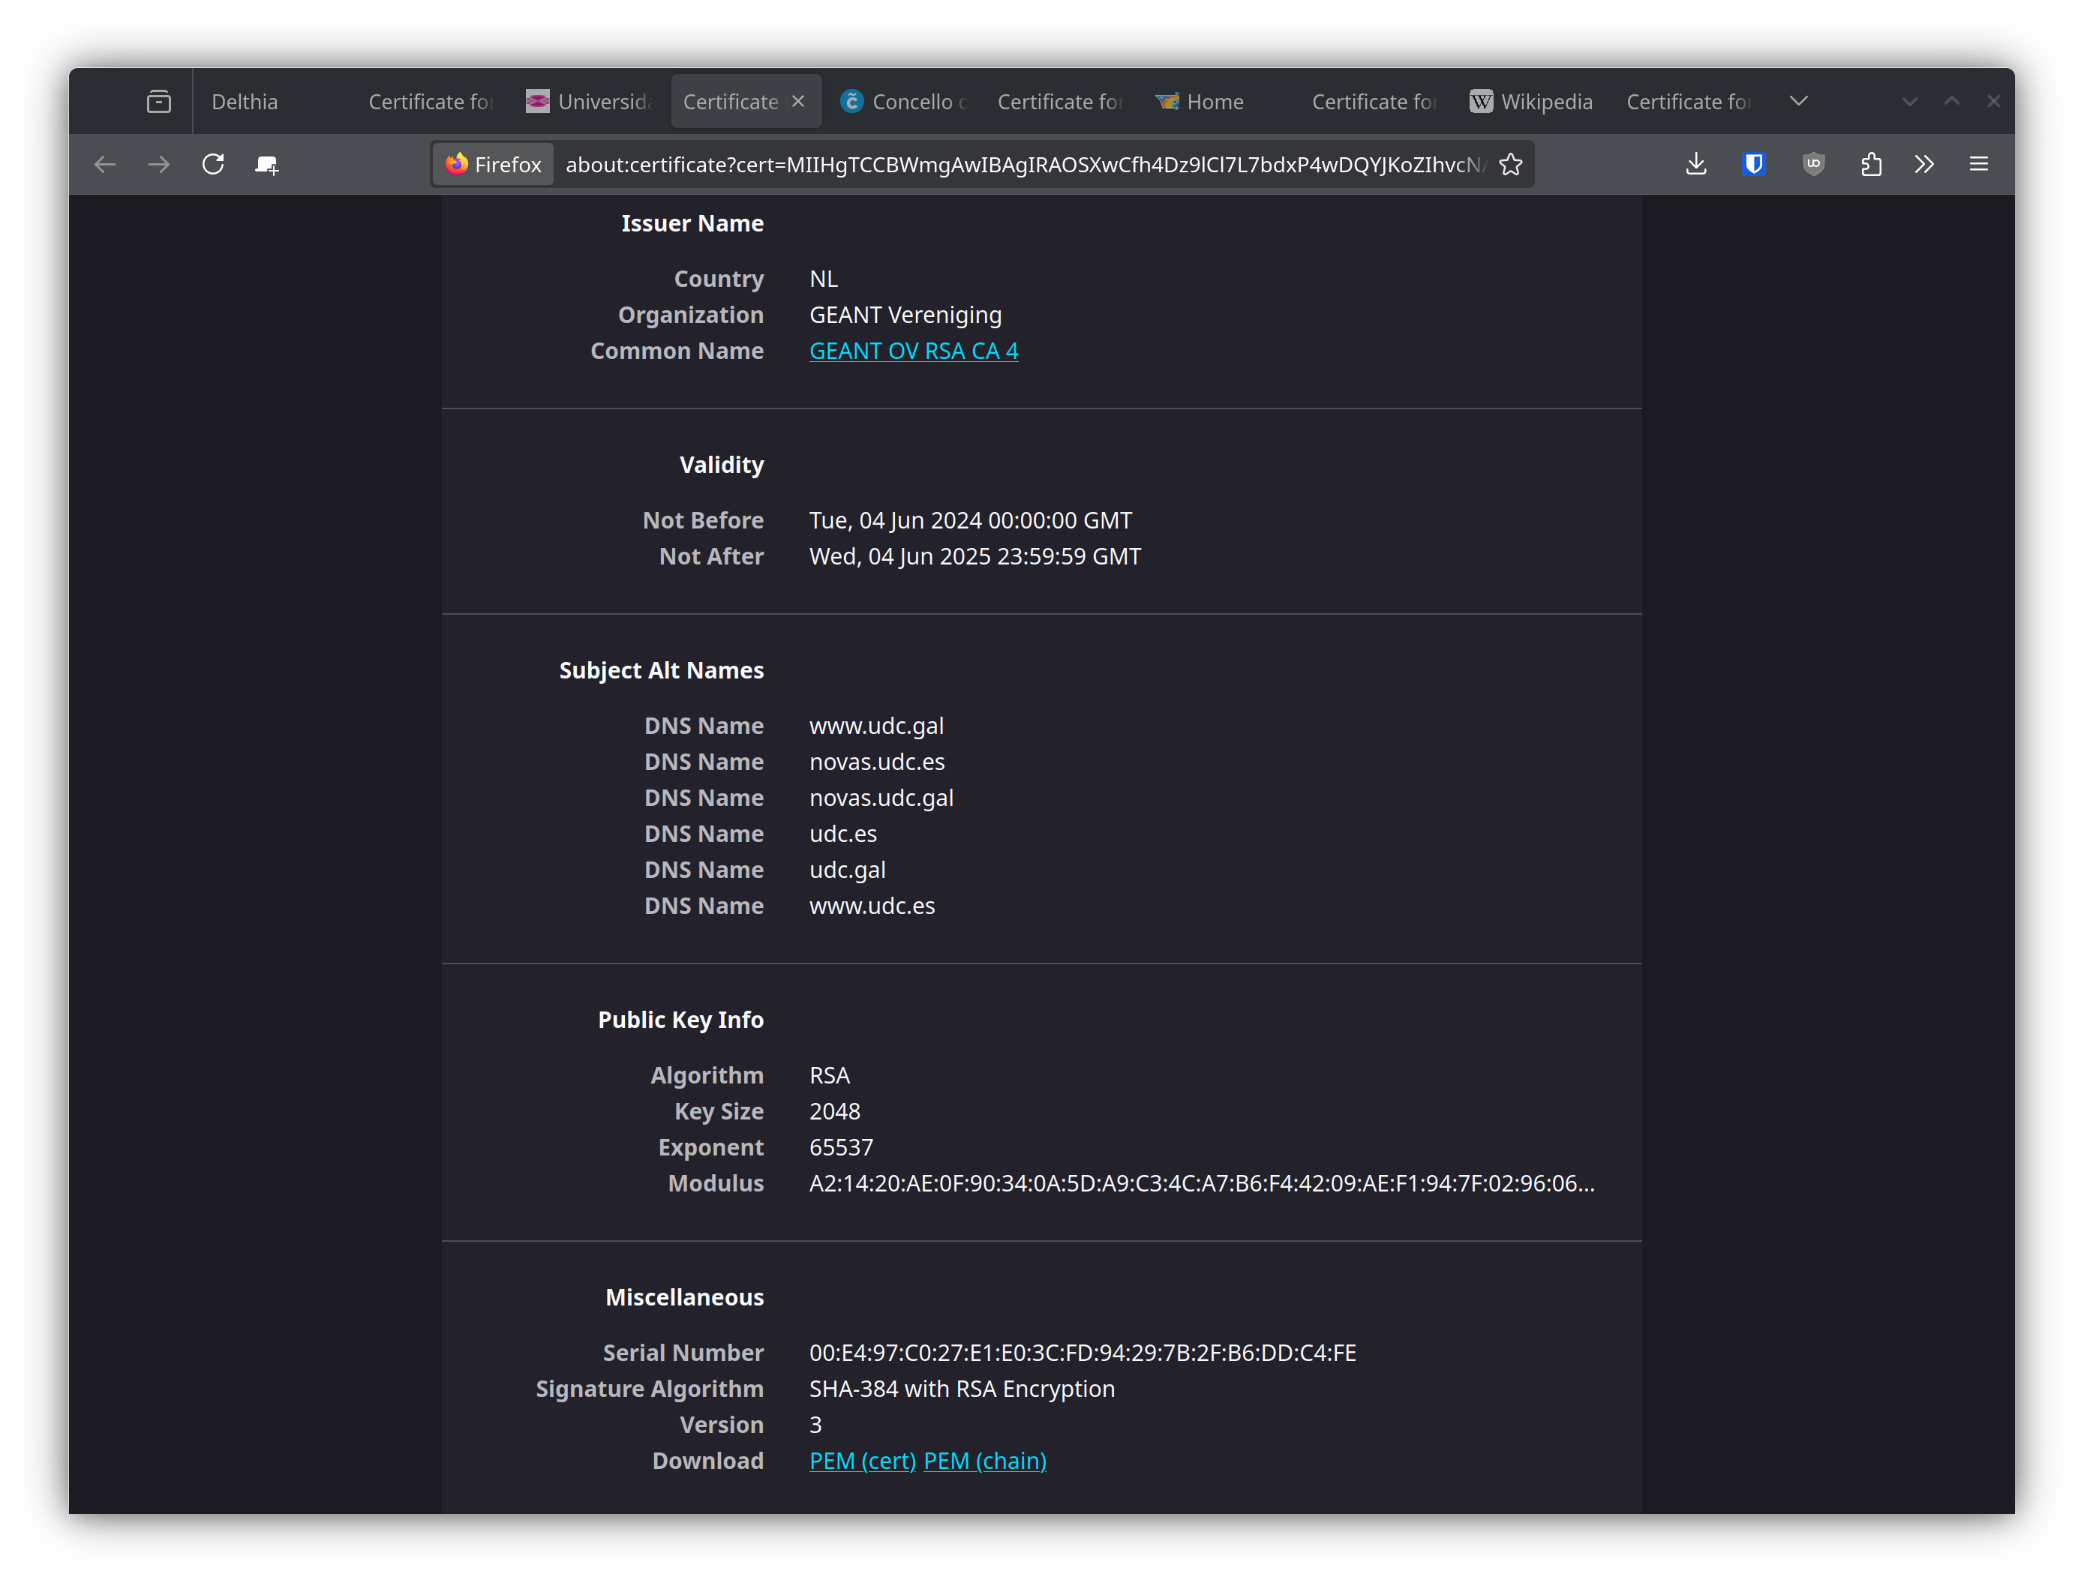
\includegraphics[width=15cm]{cert-udc.png}
    \caption{Certificado de \url{udc.es}}
\end{figure}

\begin{figure}[H]
    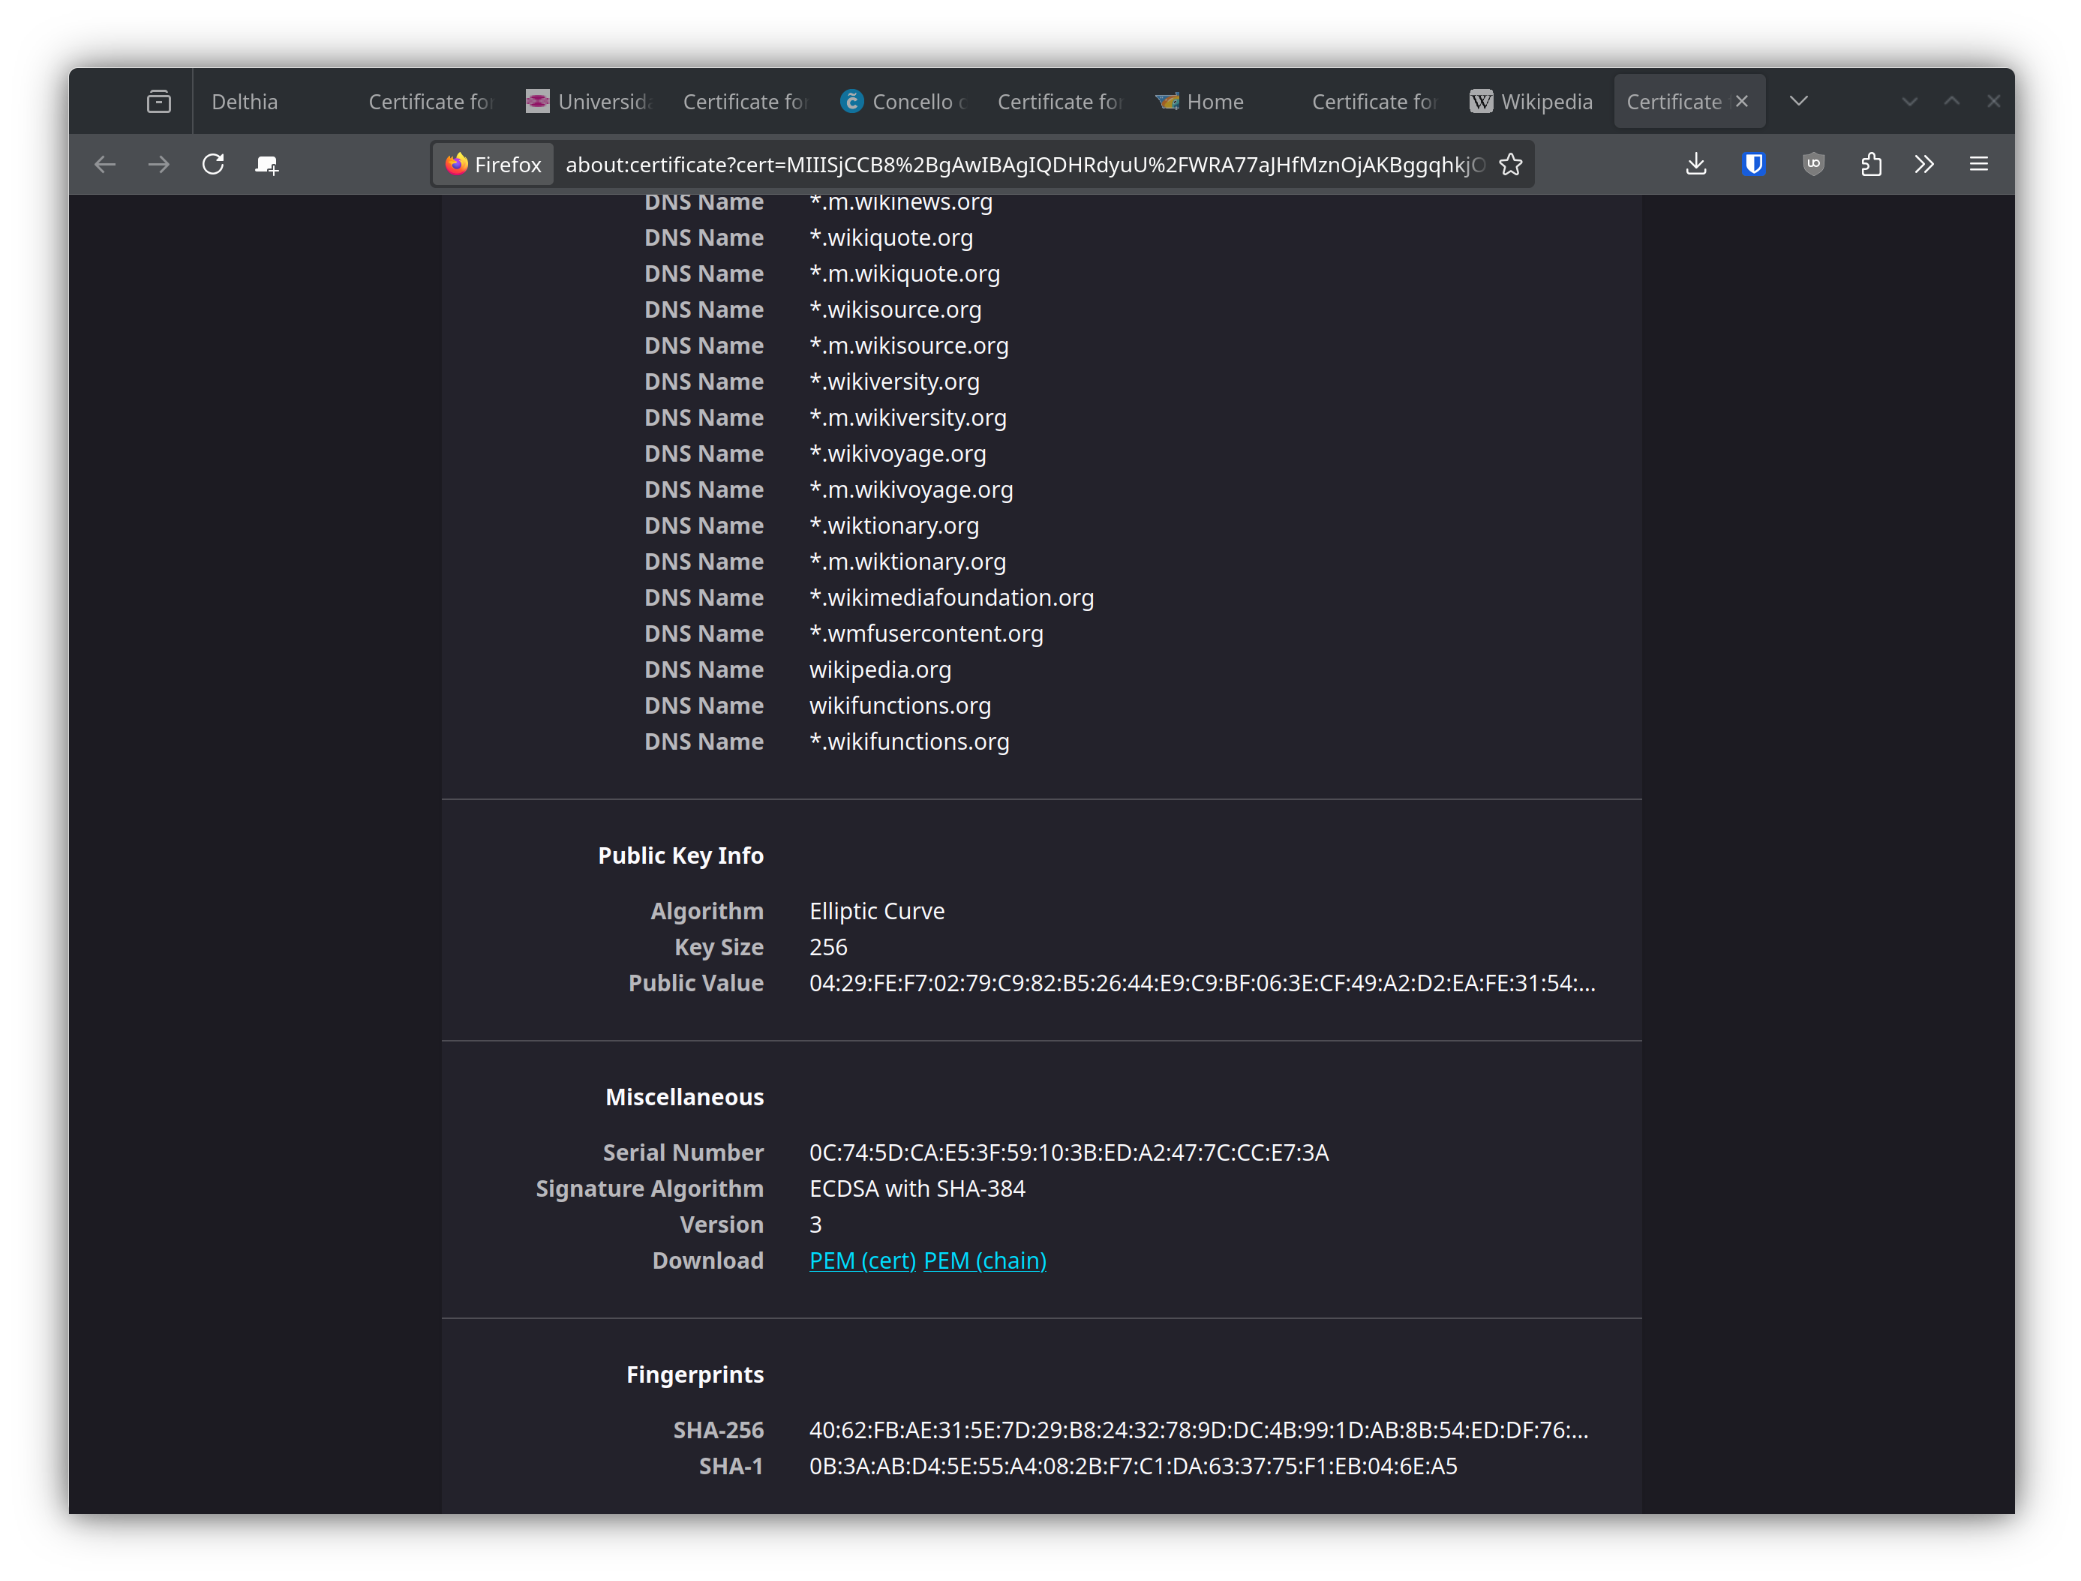
\includegraphics[width=15cm]{cert-wikipedia.png}
    \caption{Certificado de \url{wikipedia.org}}
\end{figure}

\subsubsection{Análisis con openssl}

A continuación se analizan los certificados de \url{coruna.gal} y \url{udc.es}, para lo que utiliza \texttt{OpenSSL} para descargar el certificado y ver los detalles con el comando

\begin{minted}[
frame=single,
framesep=8pt,
breaklines,
bgcolor=bgGray,
]{bash}
    openssl s_client -showcerts -servername coruna.gal -connect coruna.gal:443
\end{minted}

Es importante indicar el nombre de dominio del que se desea obtener el certificado, ya que desde un mismo servidor con la misma dirección se pueden servir varios sitios web, dependiendo de la cabecera \texttt{host}.

\subsection{Ejercicio 5}
\graphicspath{ {img/05} }

\subsubsection{Proceso para obtener certificado digital FNMT}

Lo primero que se debe hacer para obtener el certificado digital es entrar en la web de la Fábrica Nacional de Moneda y Timbre (FNMT). Una vez ahí, seleccionamos la opción “Obtener certificado digital como persona física”. Se verá en la pantalla la \ref{fig:web_ej5a}. 

\begin{figure}[H]   
    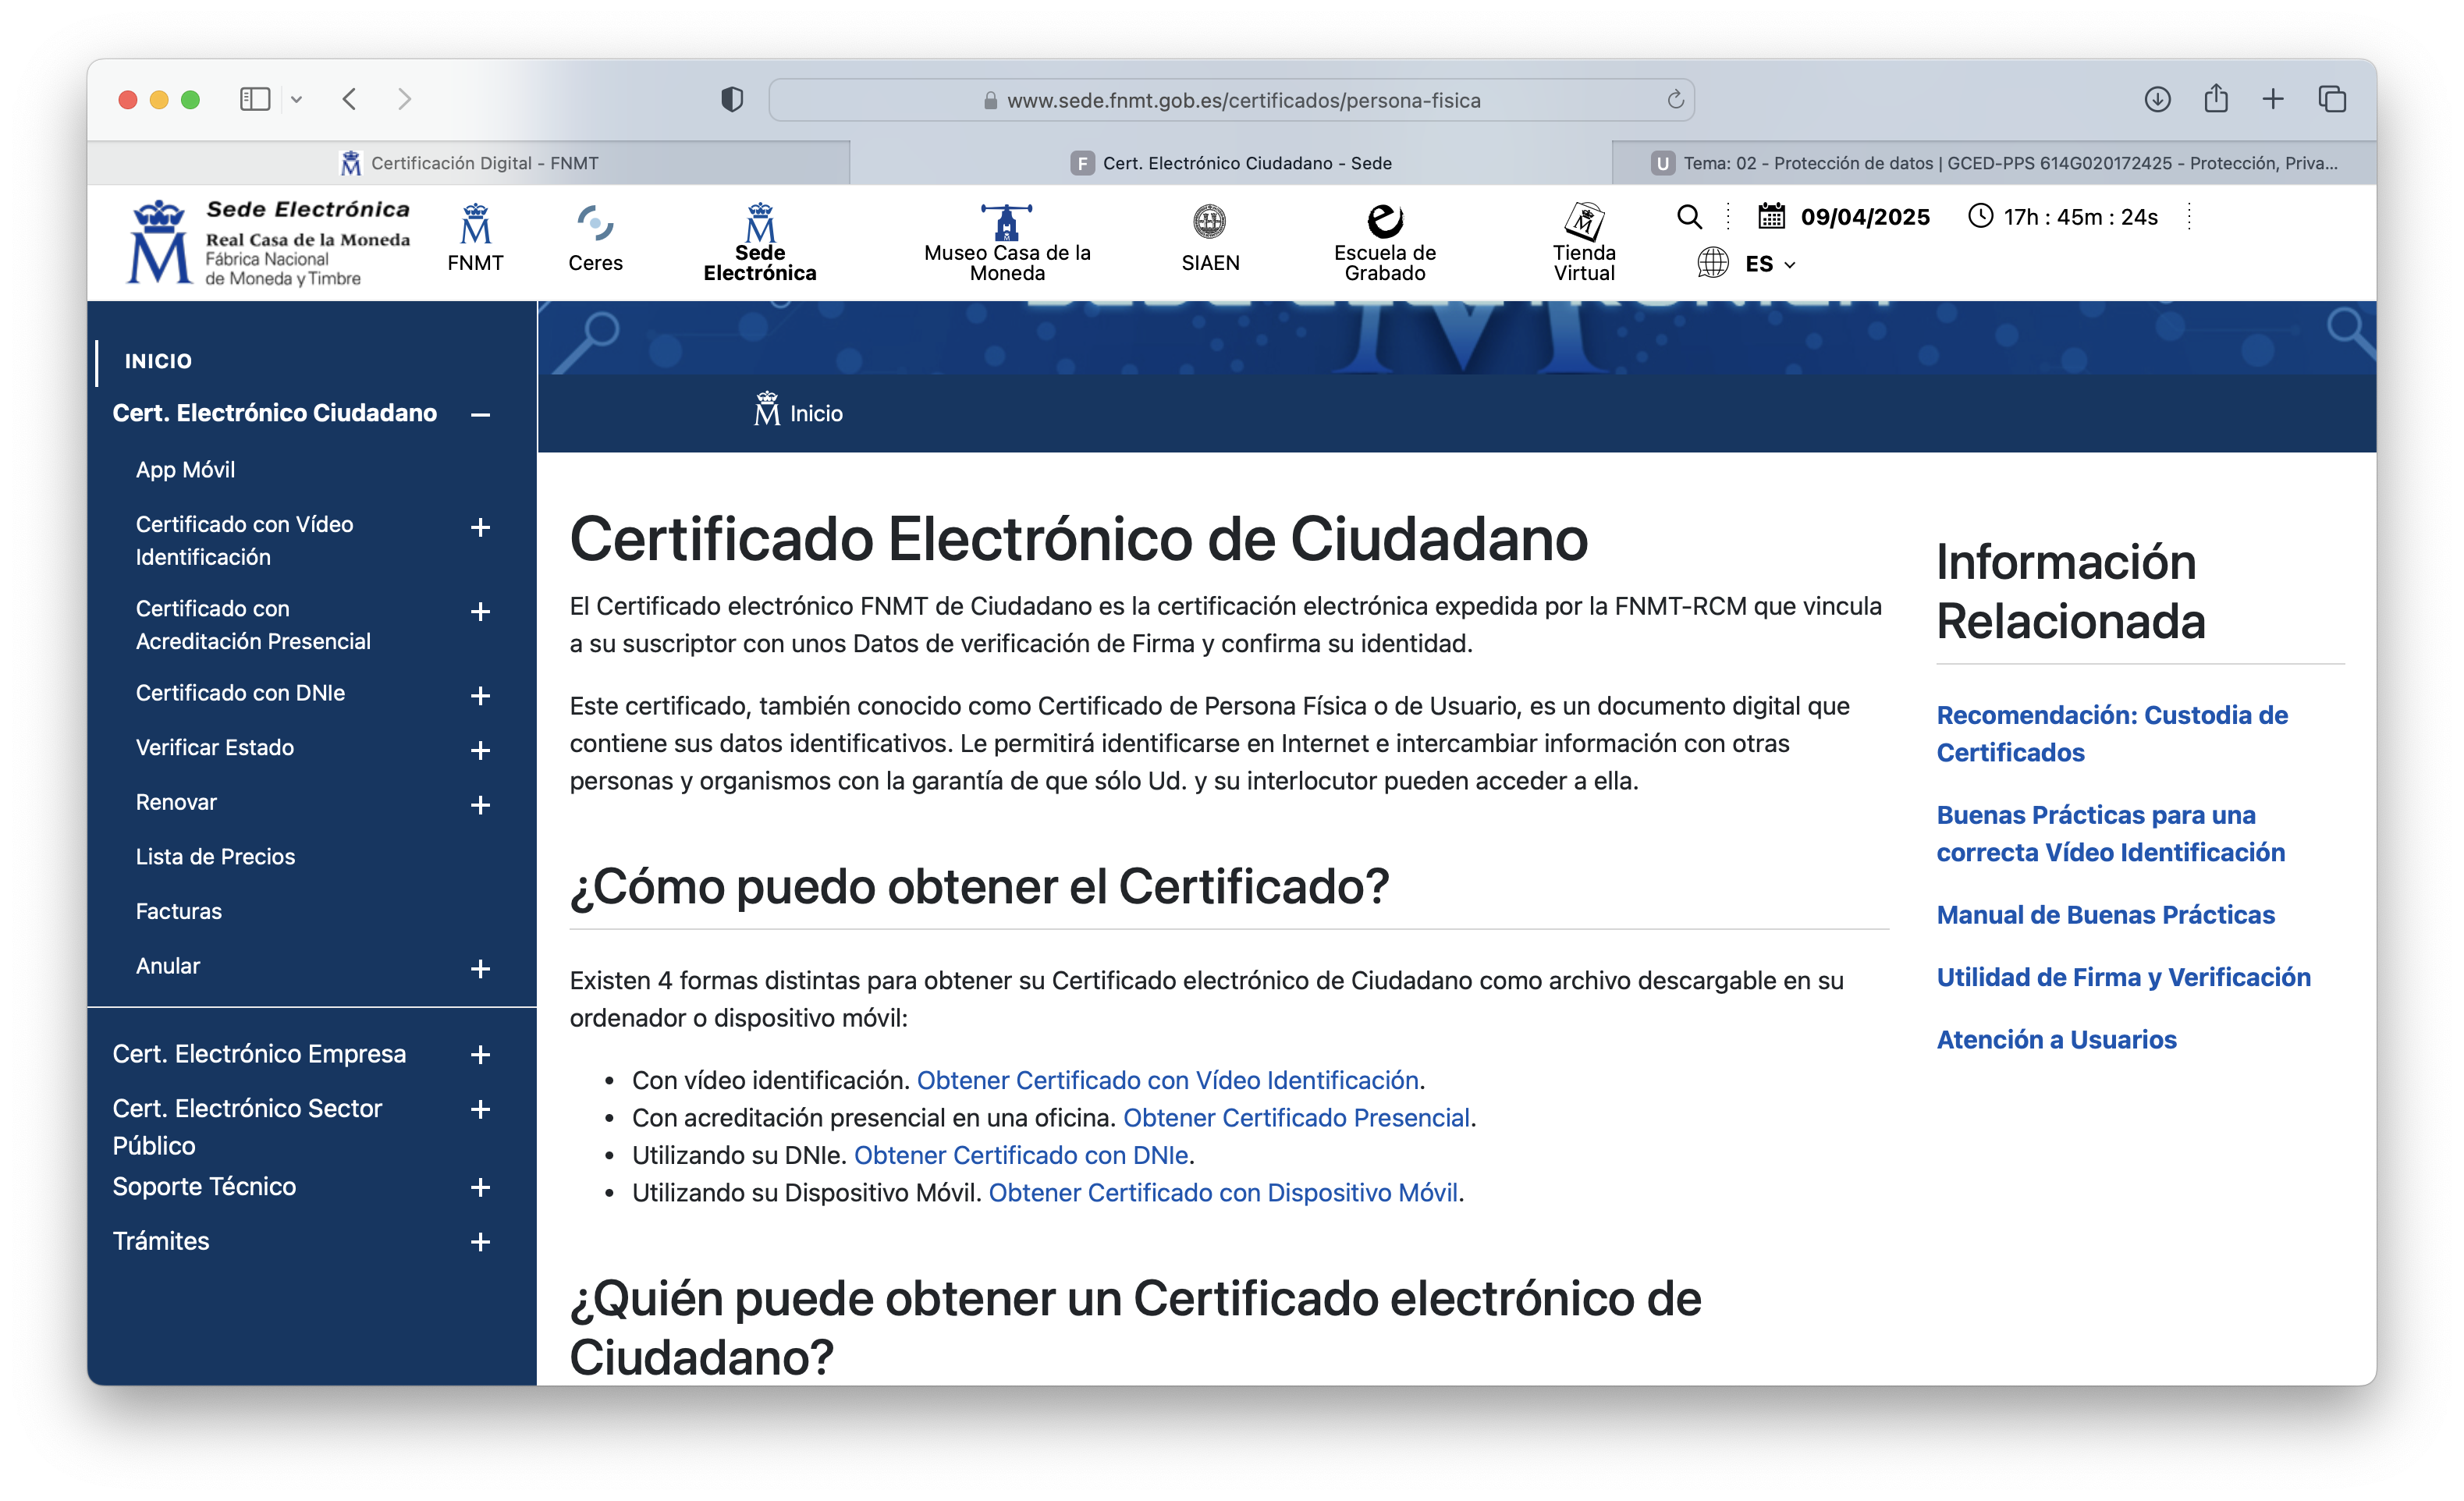
\includegraphics[width=\textwidth]{web_ej5a.png}
    \caption{Página inicio web FNMT}
    \label{fig:web_ej5a}
\end{figure}

En ella se ven las 4 formas a través de las que podemos conseguir el certificado. En nuestro caso, se eligió la opción de "Obtener certificado presencial". Una vez seleccionada la opción, como se ve en la \ref{fig:paso1}, se nos explican 4 pasos a seguir para obtener nuestro certificado. 

El paso 1 consiste en una configuración previa. Se debe instalar una aplicación para solicitar las claves necesarias en la obtención de un certificado digital. Puede ser ejecutada en cualquier navegador y sistema Operativo. Una vez descargado e instalado el software no es necesario hacer nada, este se ejecutará cuando el navegador lo requiera. En la \ref{fig:instalacion_FNMT}, se ve el final de la instalación del software. En la propia instalación se crea la contraseña, necesaria para el paso final. 

\begin{figure}[H]   
    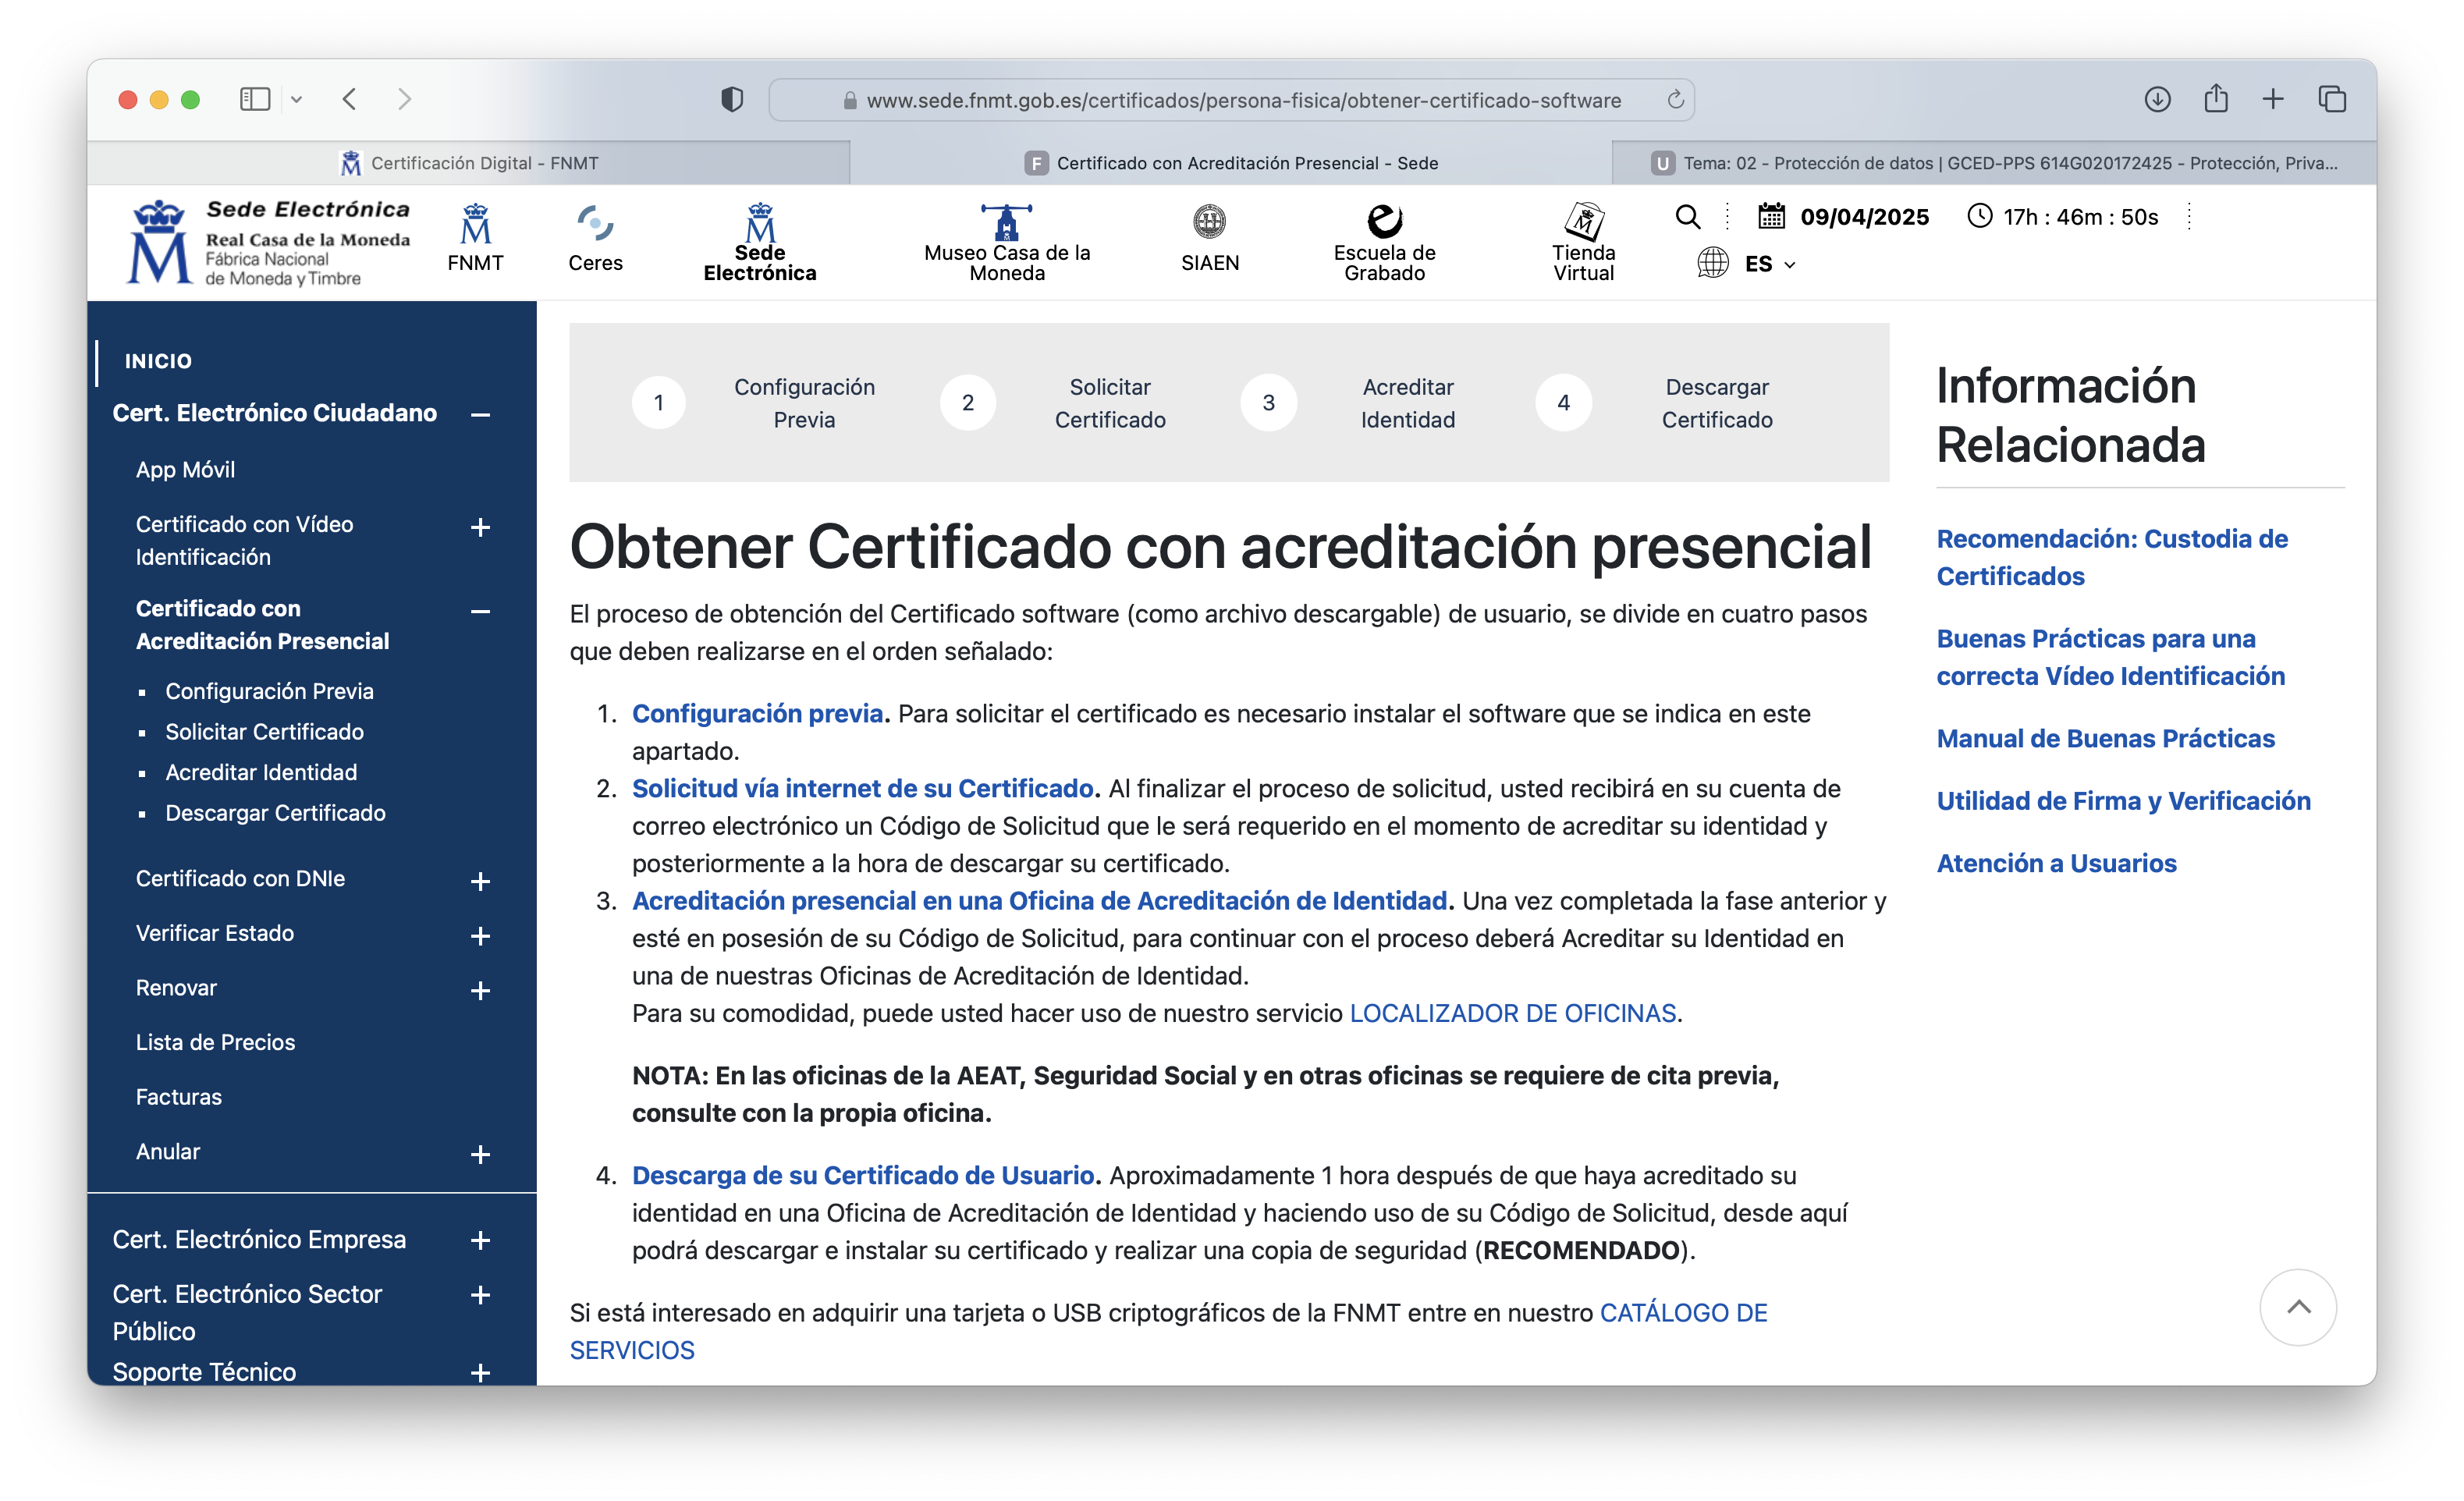
\includegraphics[width=\textwidth]{paso1_ej5a.png}
    \caption{Paso 1}
    \label{fig:paso1}
\end{figure}

\begin{figure}[H]   
    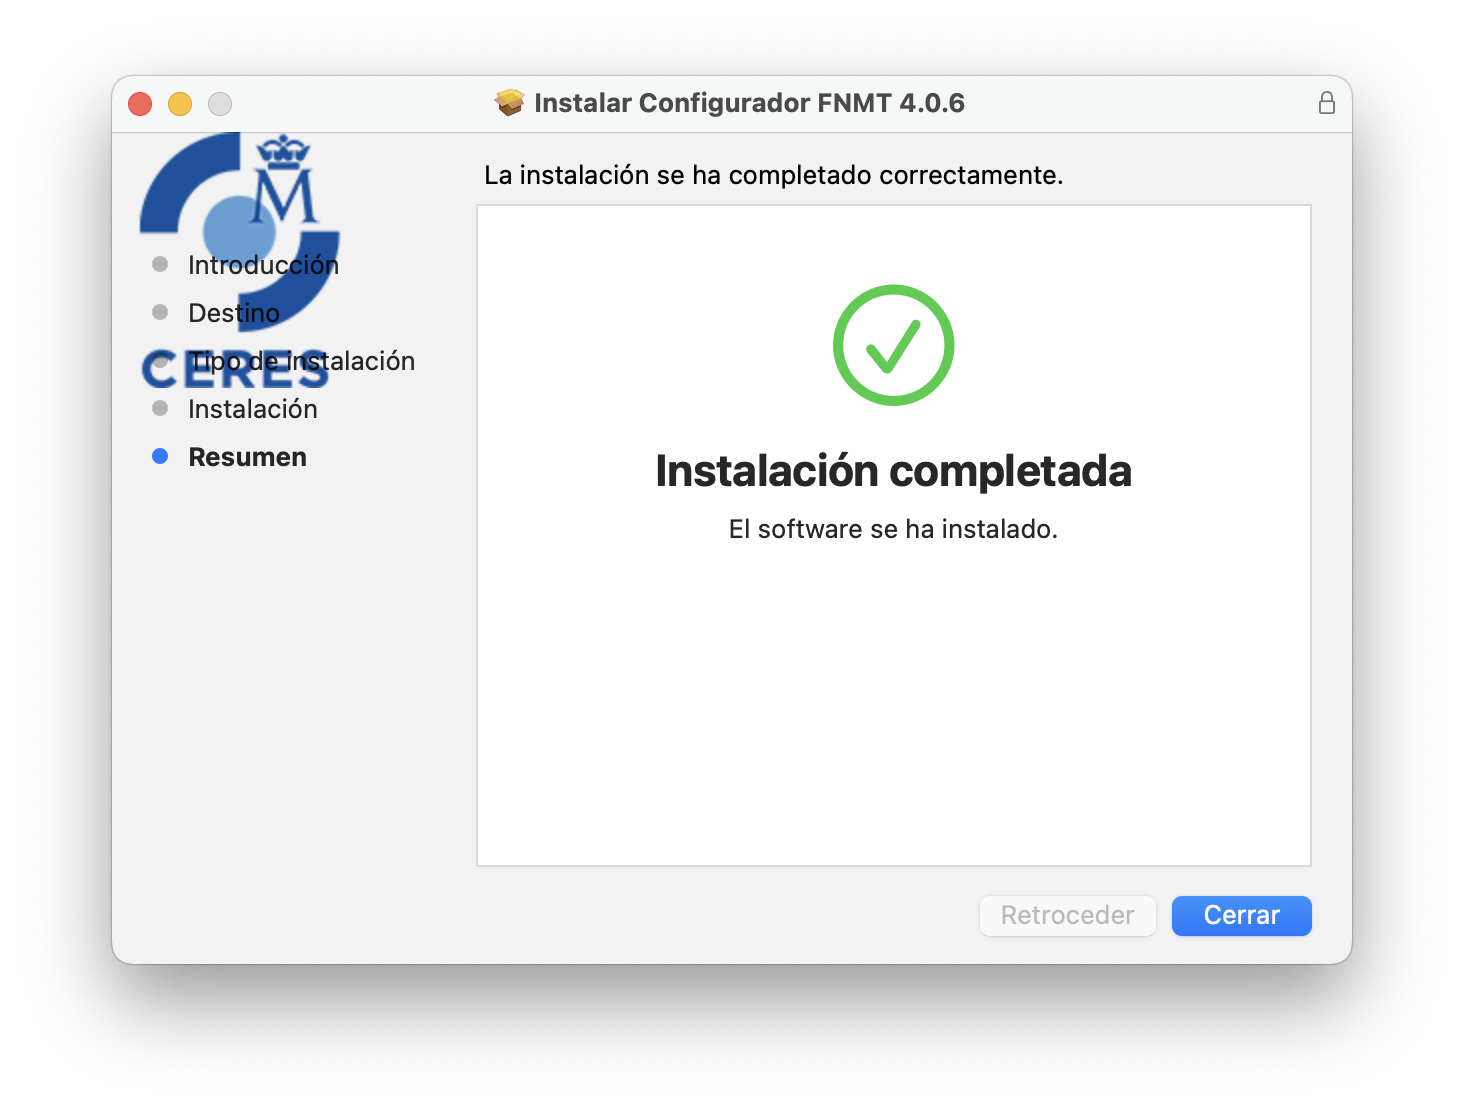
\includegraphics[width=\textwidth]{instalacion_FNMT_ej5a.png}
    \caption{Instalación software FNMT}
    \label{fig:instalacion_FNMT}
\end{figure}

Una vez instalado el software, proseguimos con el paso 2. En este paso debemos cubrir un formulario para solicitar el certificado. En la \ref{fig:paso2} se ve el formulario a cubrir. Tras la solicitud, se recibe un correo electrónico que incluye un código de solicitud. 

\begin{figure}[H]   
    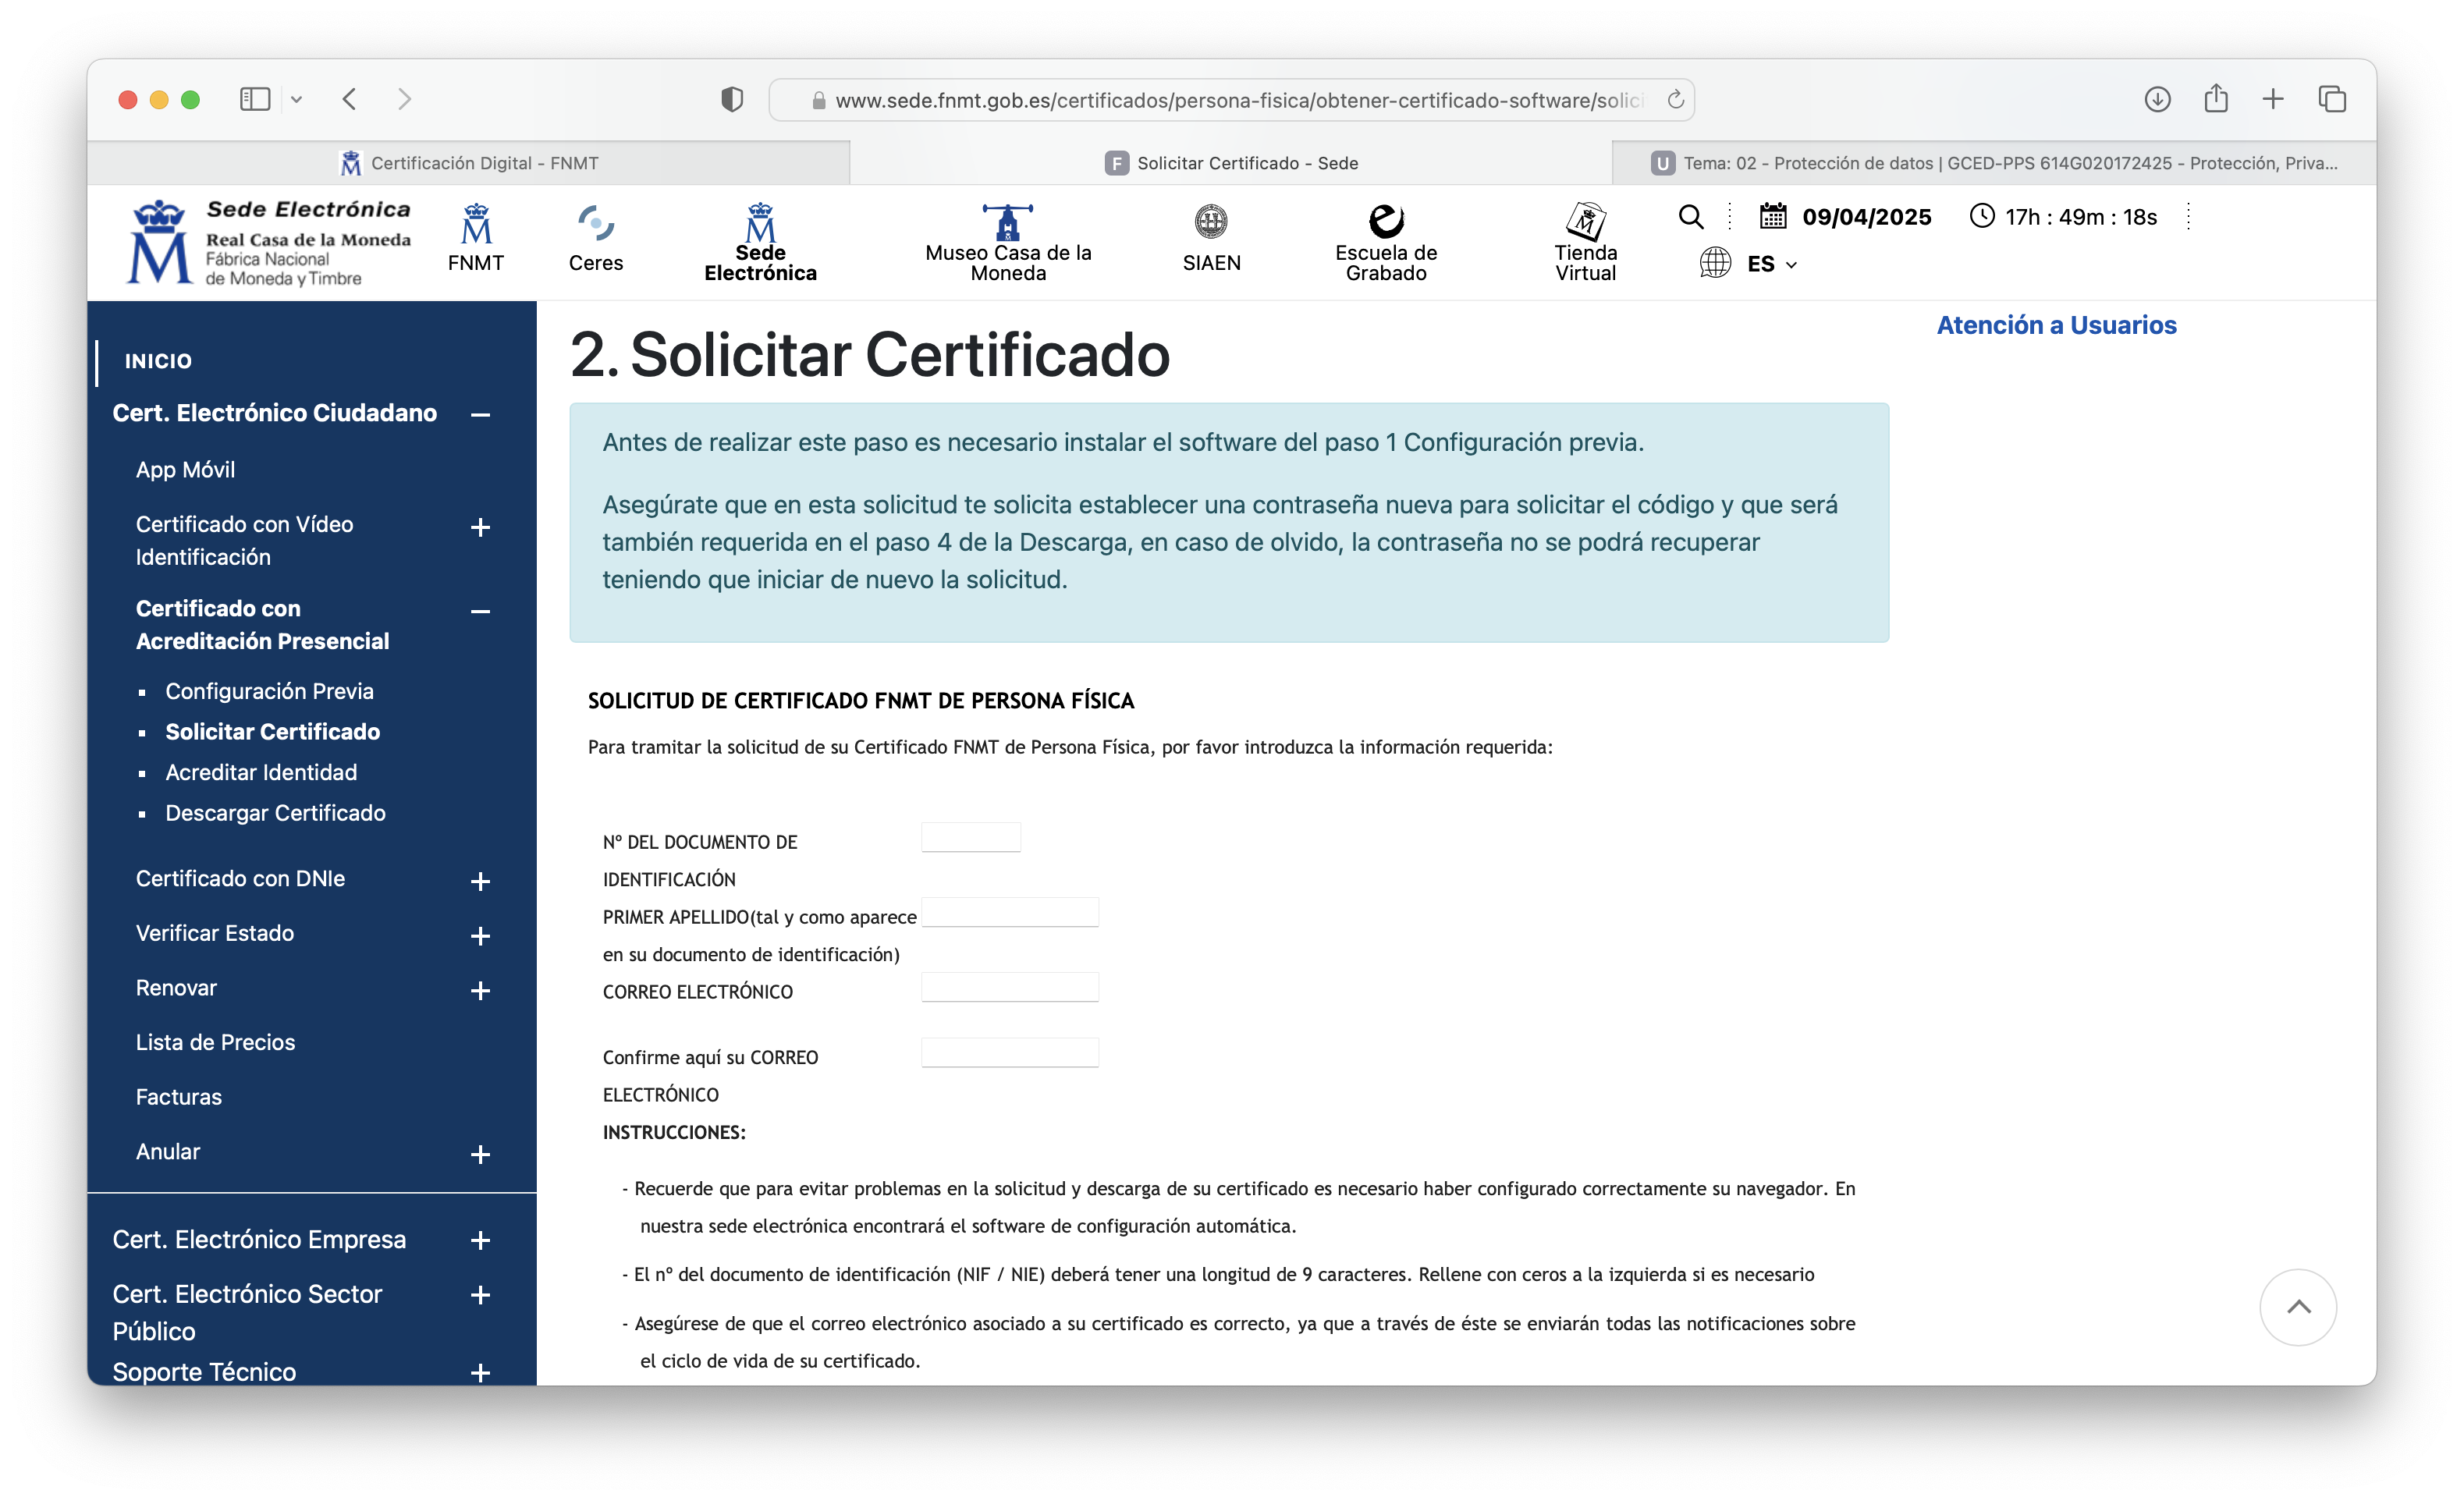
\includegraphics[width=\textwidth]{paso2_ej5a.png}
    \caption{Paso 2}
    \label{fig:paso2}
\end{figure}

El tercer paso consiste en acudir presencialmente a una oficina de registro habilitada con nuestro DNI físico y el código de solicitud obtenido en el correo electrónico del paso anterior. Allí, nos identificaron presencialmente y validaron nuestra identidad. En la página web de la FNMT se puede encontrar el mapa de la \ref{fig:mapa}, con las oficinas a las que podemos acudir, en nuestro caso, hacienda. Tras la cita, recibiremos otro correo electrónico. 

\begin{figure}[H]   
    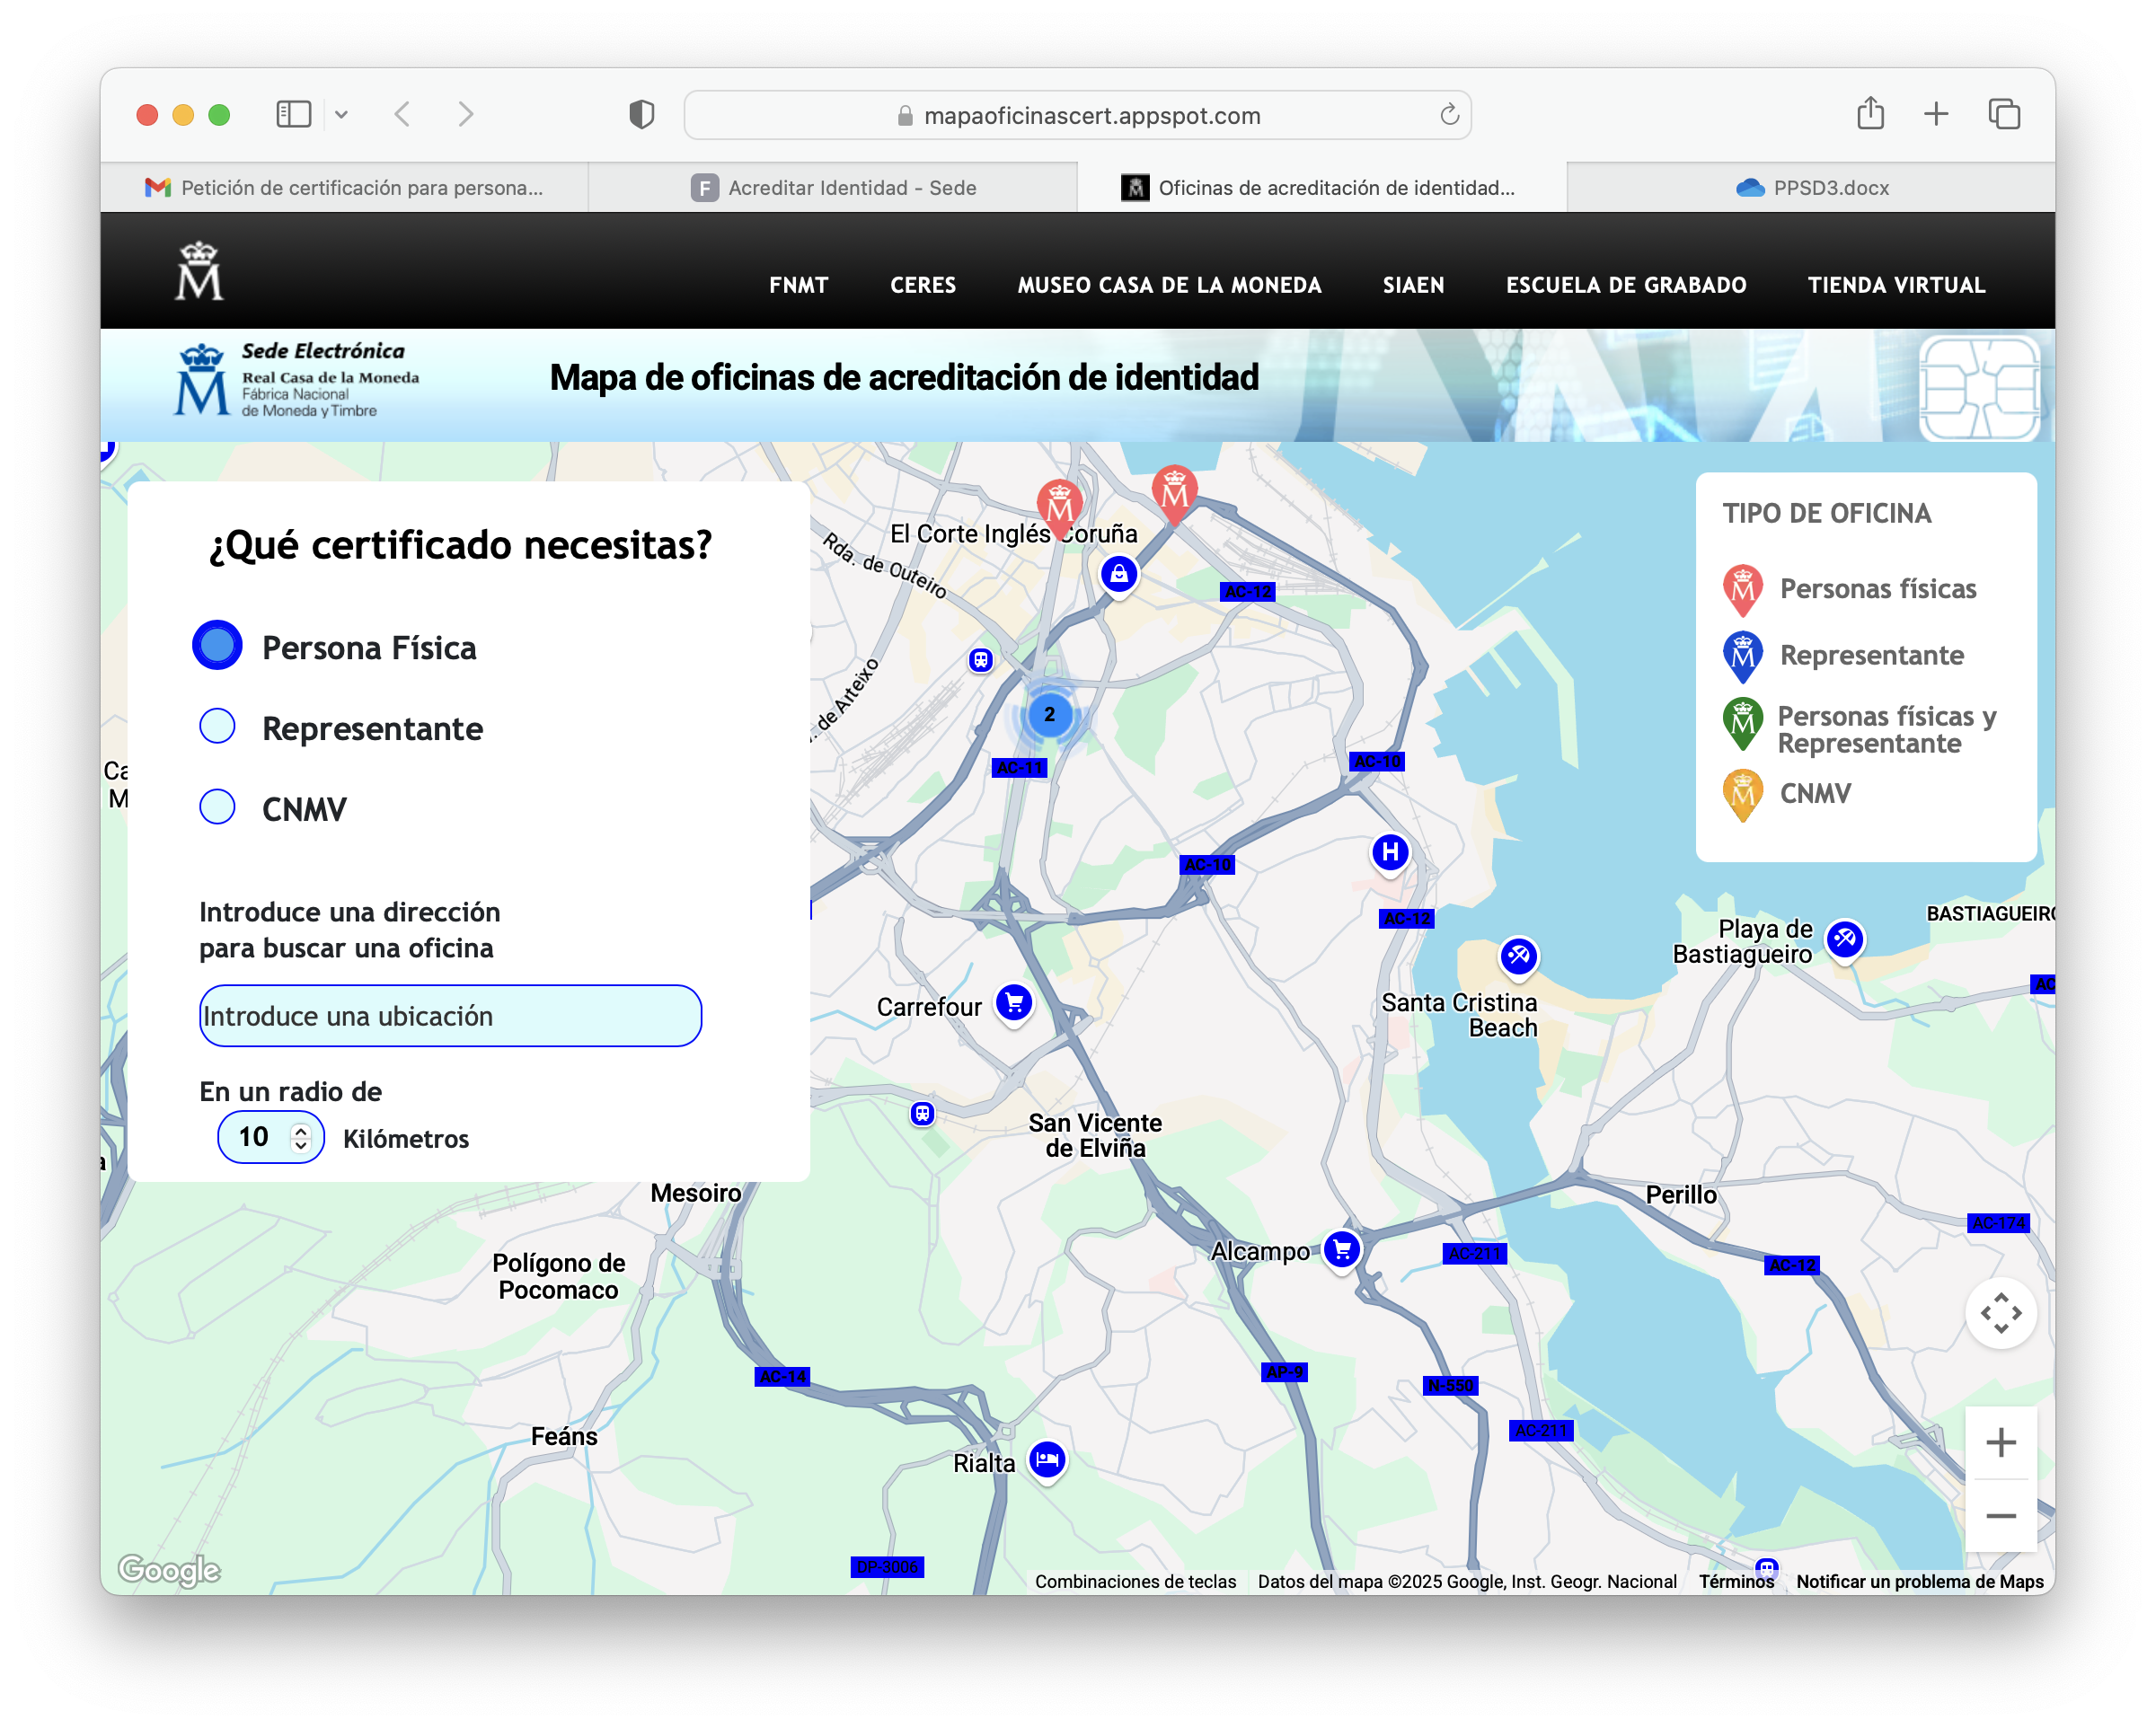
\includegraphics[width=\textwidth]{mapa_ej5a.png}
    \caption{Mapa oficinas de acreditación}
    \label{fig:mapa}
\end{figure}

El último paso consiste en descargar el certificado en el mismo navegador y equipo con el que se hizo la solicitud. En el correo electrónico recibido tras acudir a hacienda, se nos proporciona la confirmación de nuestra solicitud, así como el enlace al formulario de la \ref{fig:paso4}. Una vez cubierto, el navegador instala el certificado, vinculando la clave privada local con el certificado emitido por la FNMT. Se debe ver un mensaje como el de la \ref{fig:fin_instalacion}. Es recomendable descargar el certificado en nuestro dispositivo.  

\begin{figure}[H]   
    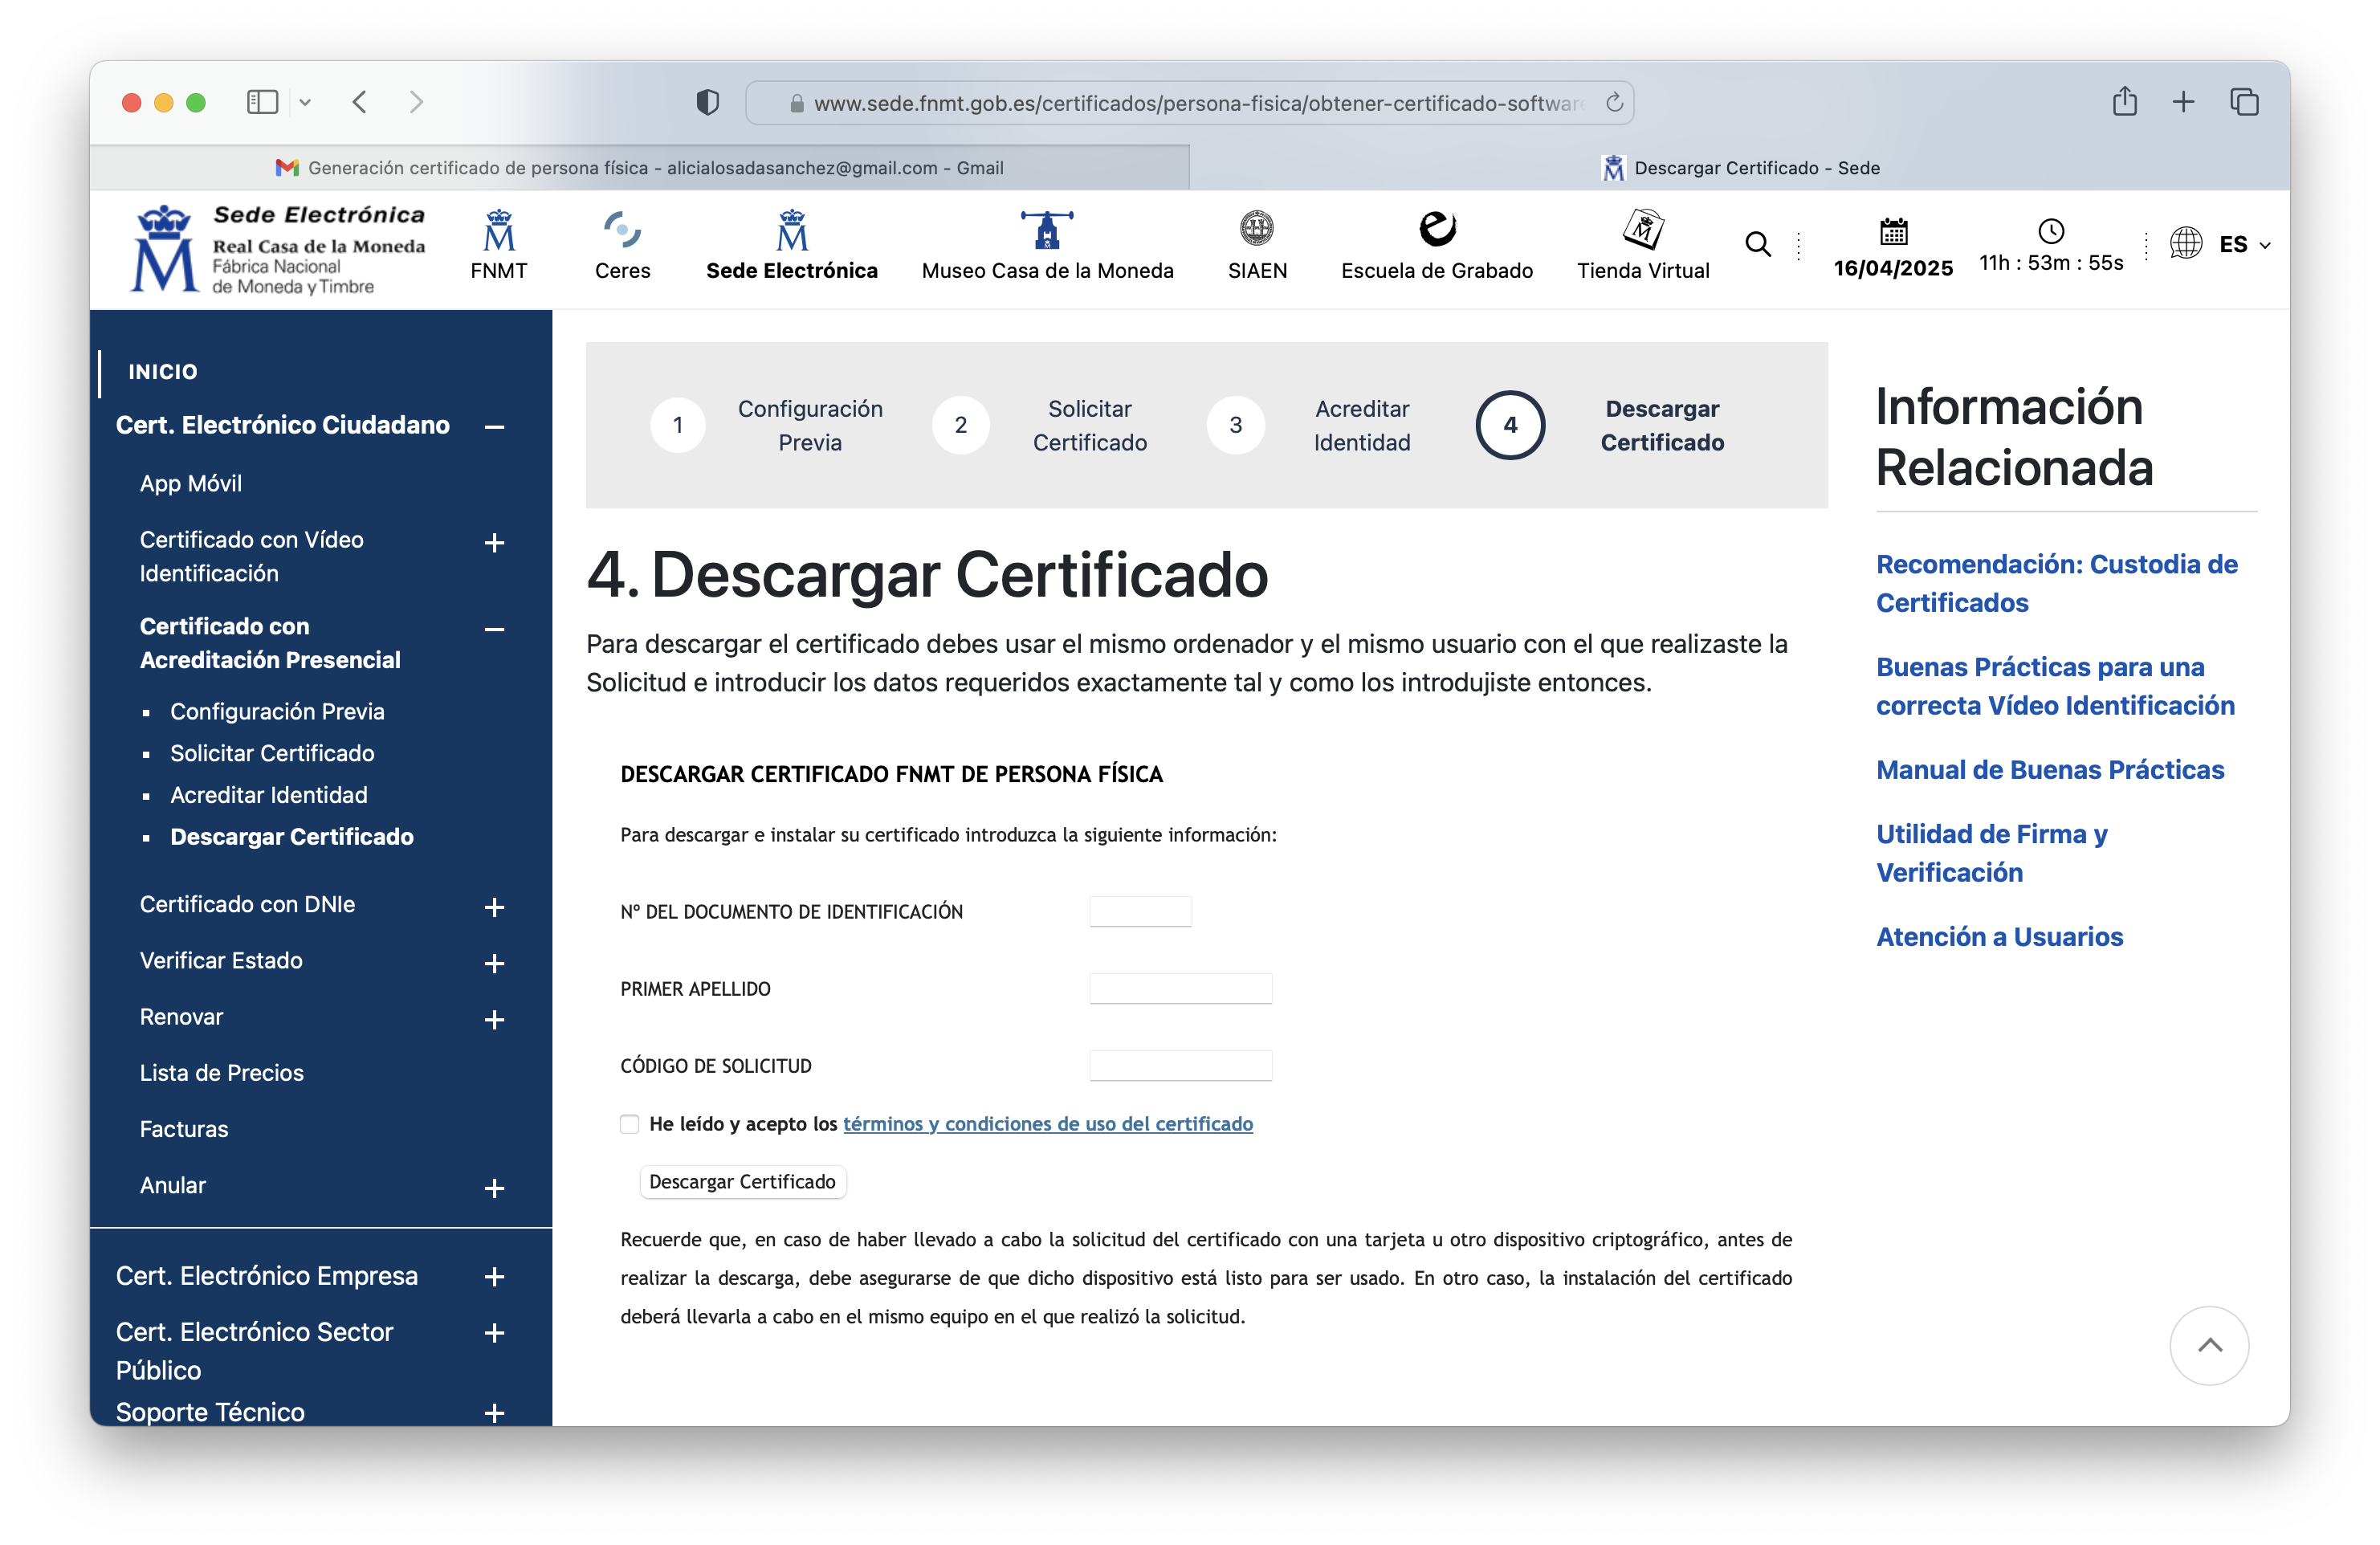
\includegraphics[width=\textwidth]{paso4_ej5a.png}
    \caption{Paso 4}
    \label{fig:paso4}
\end{figure}

\begin{figure}[H]   
    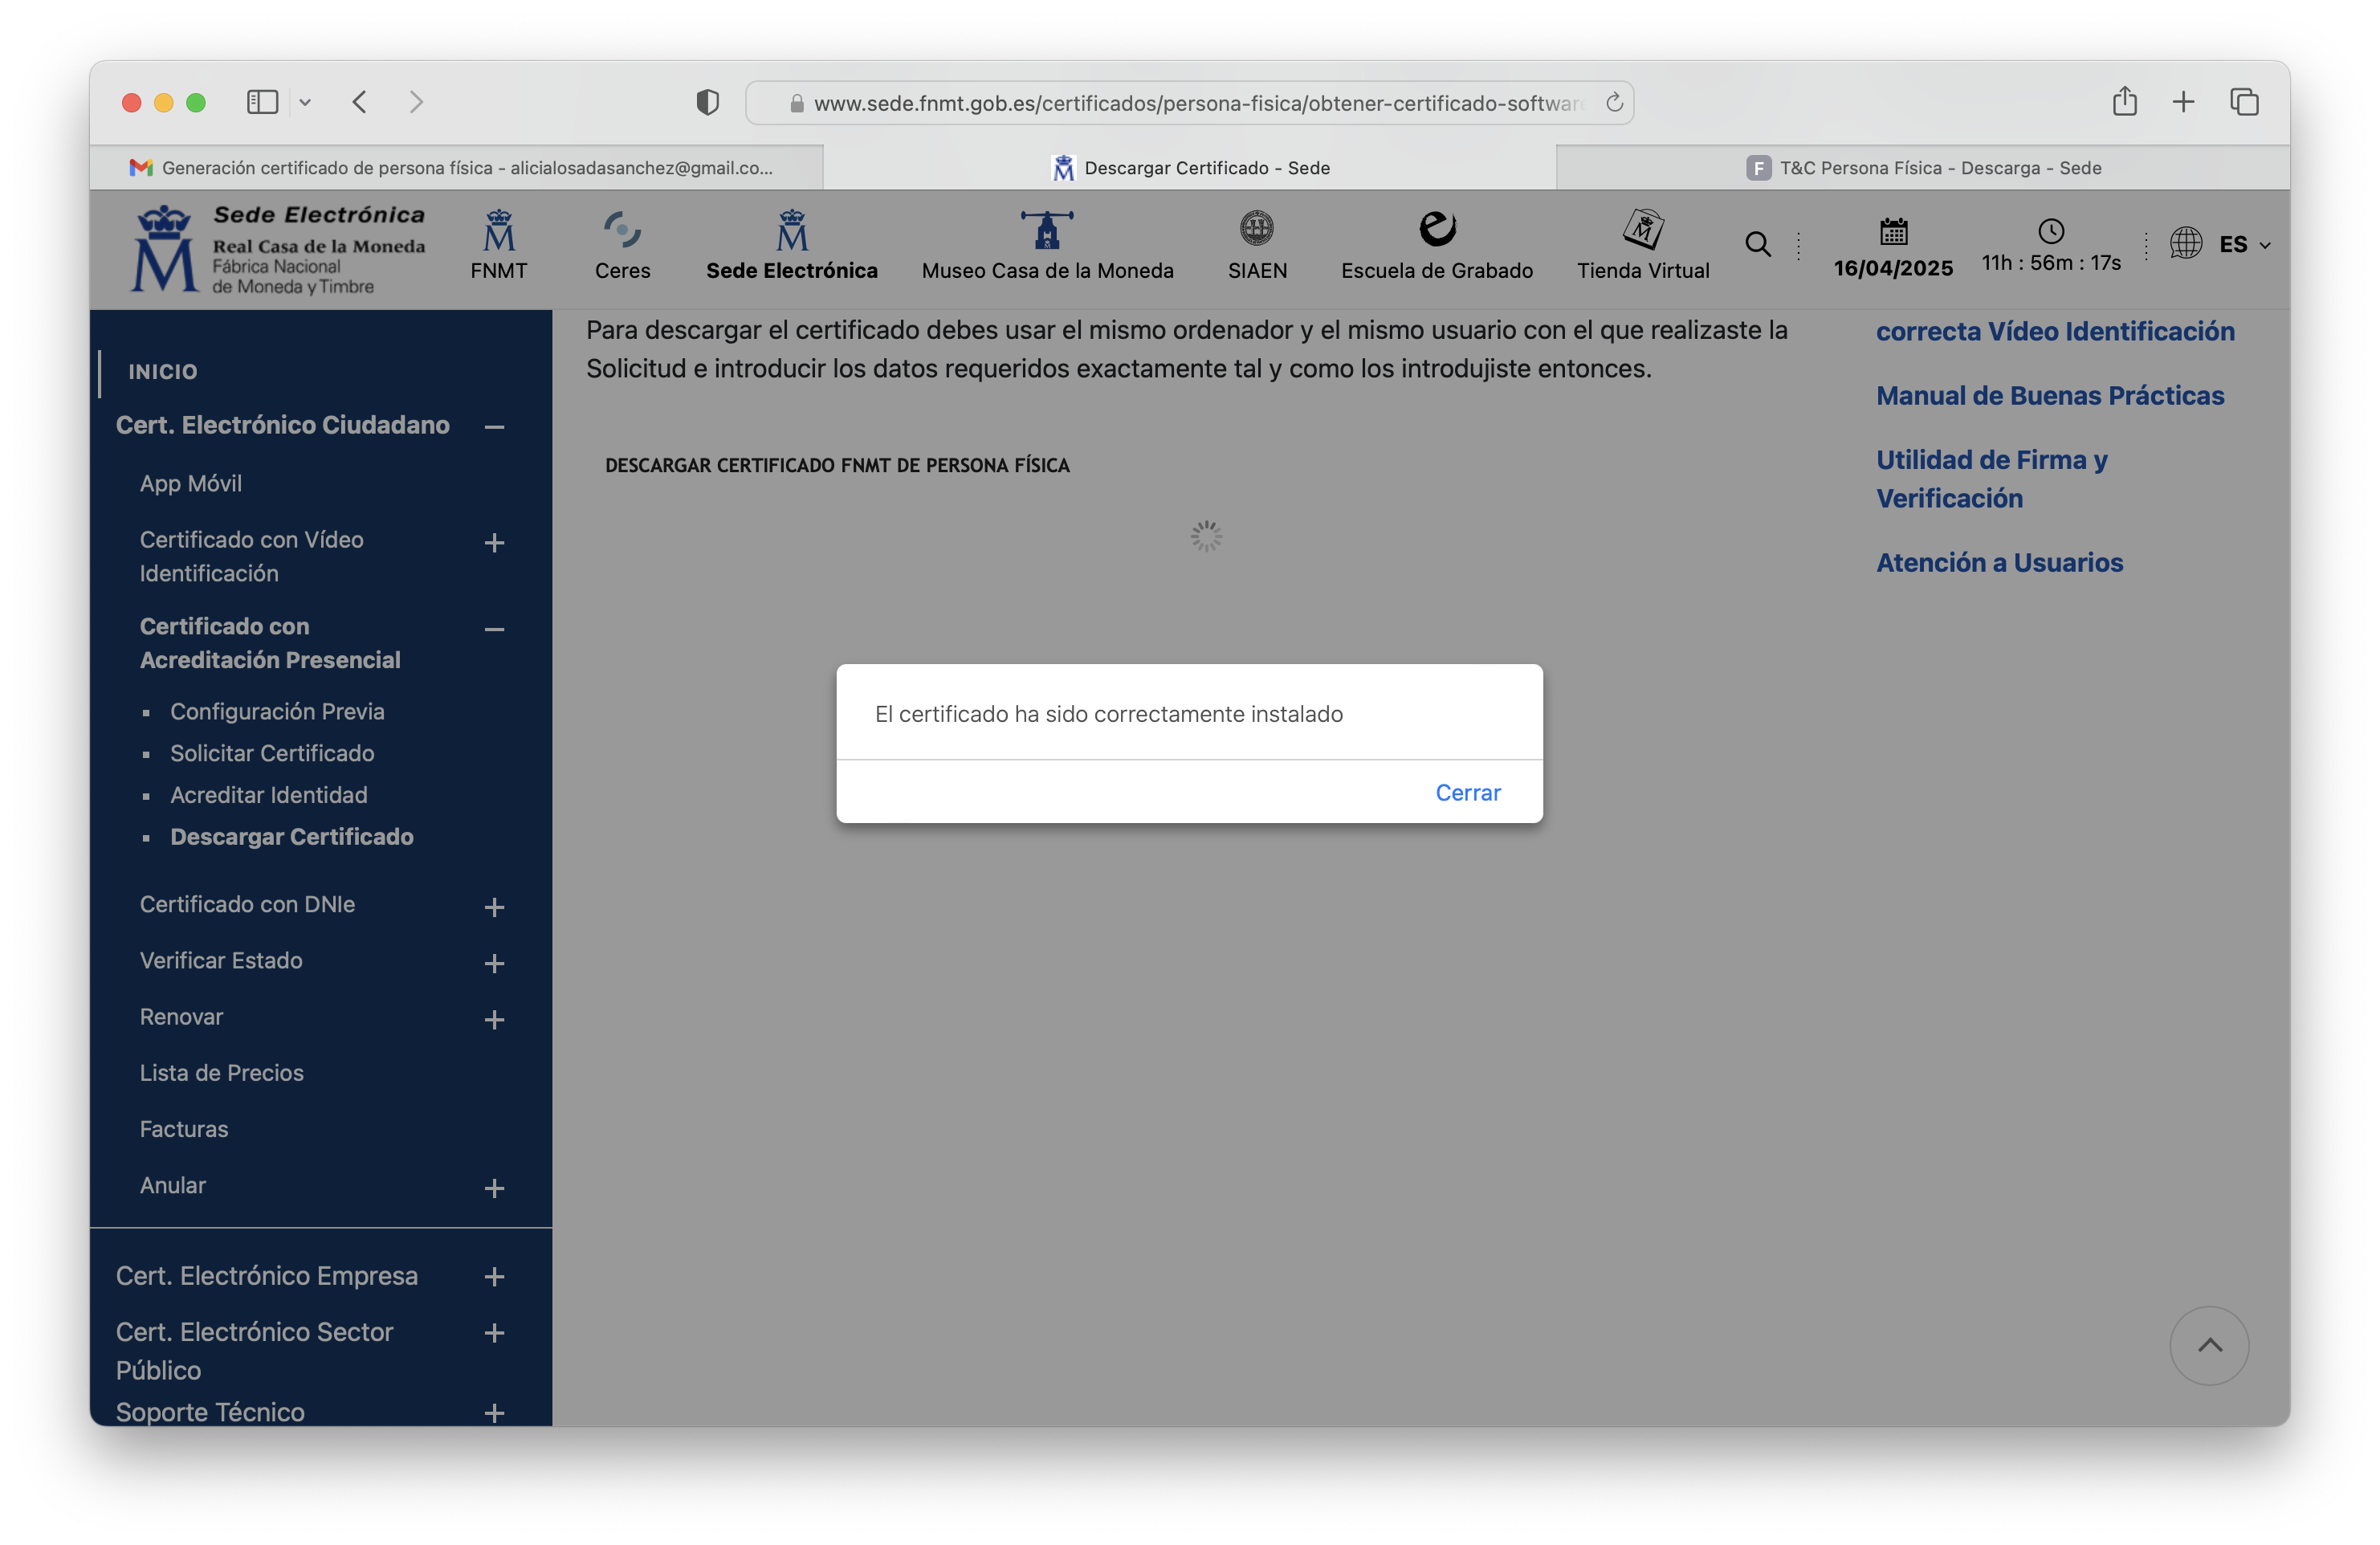
\includegraphics[width=\textwidth]{fin_instalacion_ej5a.png}
    \caption{Fin instalación certificado}
    \label{fig:fin_instalacion}
\end{figure}

Las claves se generan en el propio navegador del usuario en el momento en que se realiza la solicitud del certificado digital en la web de la FNMT. Específicamente, el navegador crea un par de claves: una clave pública, que se envía a la Autoridad Certificadora (CA), y una clave privada, que nunca abandona el equipo del usuario.  

Esta clave privada se almacena localmente en el almacén de certificados del navegador o del sistema operativo, dependiendo del navegador utilizado. Por ejemplo, en Firefox se guarda en su propio almacén interno, mientras que en navegadores como Chrome o Edge en Windows, se almacena en el almacén de certificados del sistema operativo. 


\subsubsection{Análisis campos clave pública OpenSSL}



\section{PGP y S/MIME}
\subsection{Ejercicio 6}
\graphicspath{ {img/06} }

GPG, o GnuPGP, es la implementación de GNU del estándar de criptografía PGP. Con el comando \texttt{gpg} se pueden generar claves, gestionar claves y firmar, cifrar, descifrar y comprobar la firma de documentos encriptados con PGP.

Para generar un par de claves se puede utilizar el siguiente comando:
\begin{minted}[
    frame=single,
    framesep=8pt,
    breaklines,
    bgcolor=bgGray
]{bash}
    gpg --gen-key
\end{minted}

que preguntará información sobre el usuario para generar la clave, concretamente:
\begin{itemize}
    \item{Nombre}
    \item{Direccion de correo electrónico}
    \item{Contraseña para las claves}
\end{itemize}

Sin embargo, en la captura se muestra la generación de las claves con \texttt{gpg --full-gen-key}, que permite generar la clave de manera más configurable, indicando también el algoritmo de las claves y la caducidad de las mismas

\begin{figure}[H]
    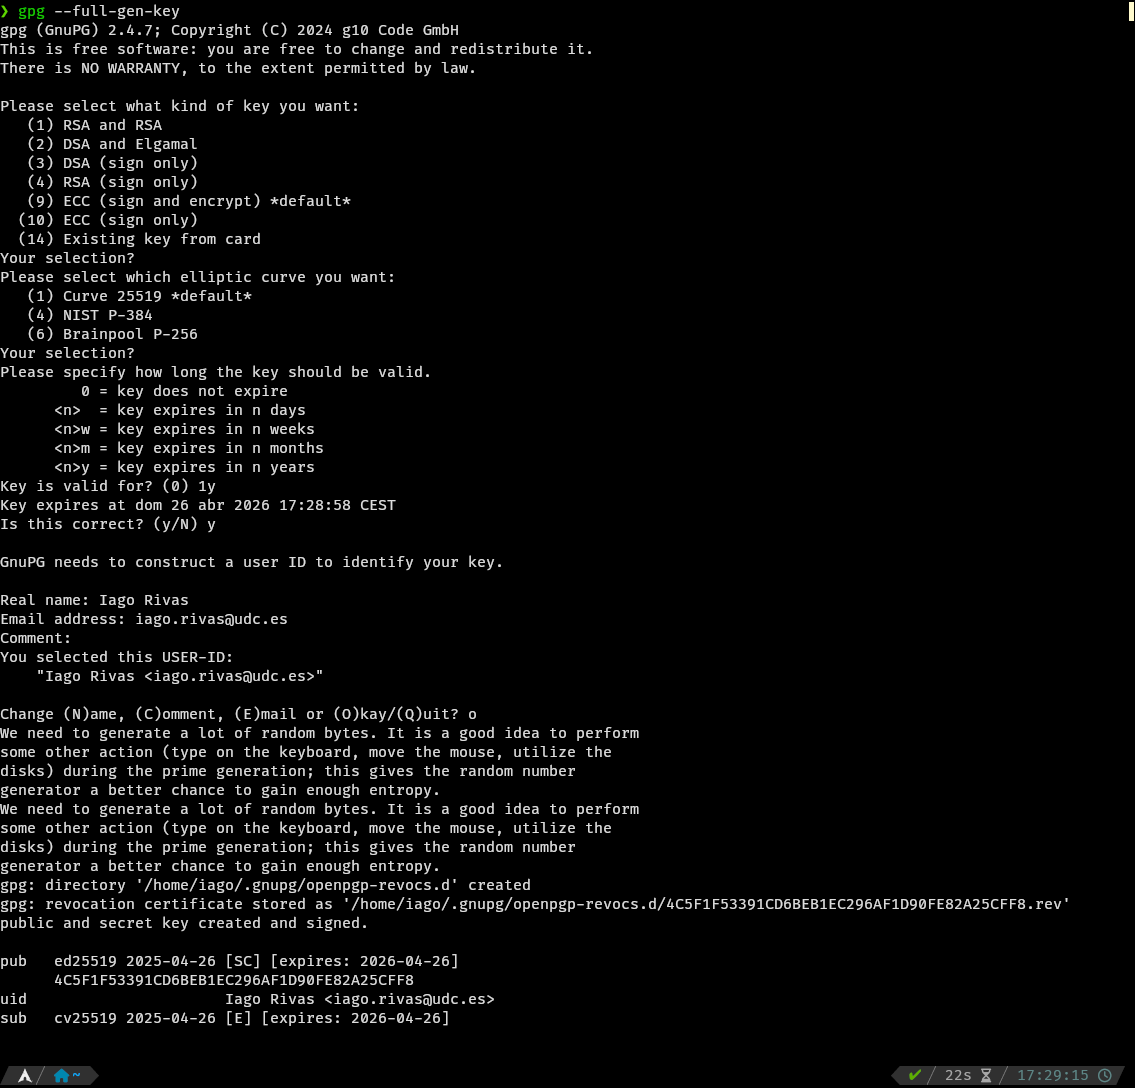
\includegraphics[width=\textwidth]{gpg-genkey.png}
    \caption{Generación del par de claves con \texttt{gpg}}
\end{figure}

Debido a la versatilidad de la criptografía de clave pública, no es neceario que todas las partes tengan claves generadas con el mismo algoritmo. En la captura se selecciona una clave de curva elíptica, pero es perfectamente factible que otra de las claves del grupo utilice RSA, ya que en ningún momento se usan las claves de más de una parte a la vez, se cifra con la clave pública del destinatario y se cifra con la privada del remitente.

Una vez generadas las claves, es necesario exportarlas, para poder compartirlas. Thunderbird comparte automáticamente la clave pública al enviar un correo, pero necesitaremos las claves públicas del resto de integrantes para poder empezar la conversación. Para exportar las claves se puede utilizar el comando:

\begin{minted}[
    frame=single,
    framesep=8pt,
    breaklines,
    bgcolor=bgGray
]{bash}
    gpg --output 2_Rivas_Moar,_Iago.asc --armor --export iago.rivas@udc.es
\end{minted}

La opción \texttt{--armor} hace que se exporte una representación en ASCII de la clave, y simplemente es necesario indicar la clave que se quiere exportar por su correo electrónico o con el ID. Compartir la clave sería cuestión de enviarla por correo electrónico u otro medio.

Si quisiéramos copiar el par de claves completo a otro ordenador, para poder utilizarla en varios ordenadores, tendríamos que cambiar la opción \texttt{--export} por \\ \texttt{--export-secret-keys}.

\begin{figure}[H]
    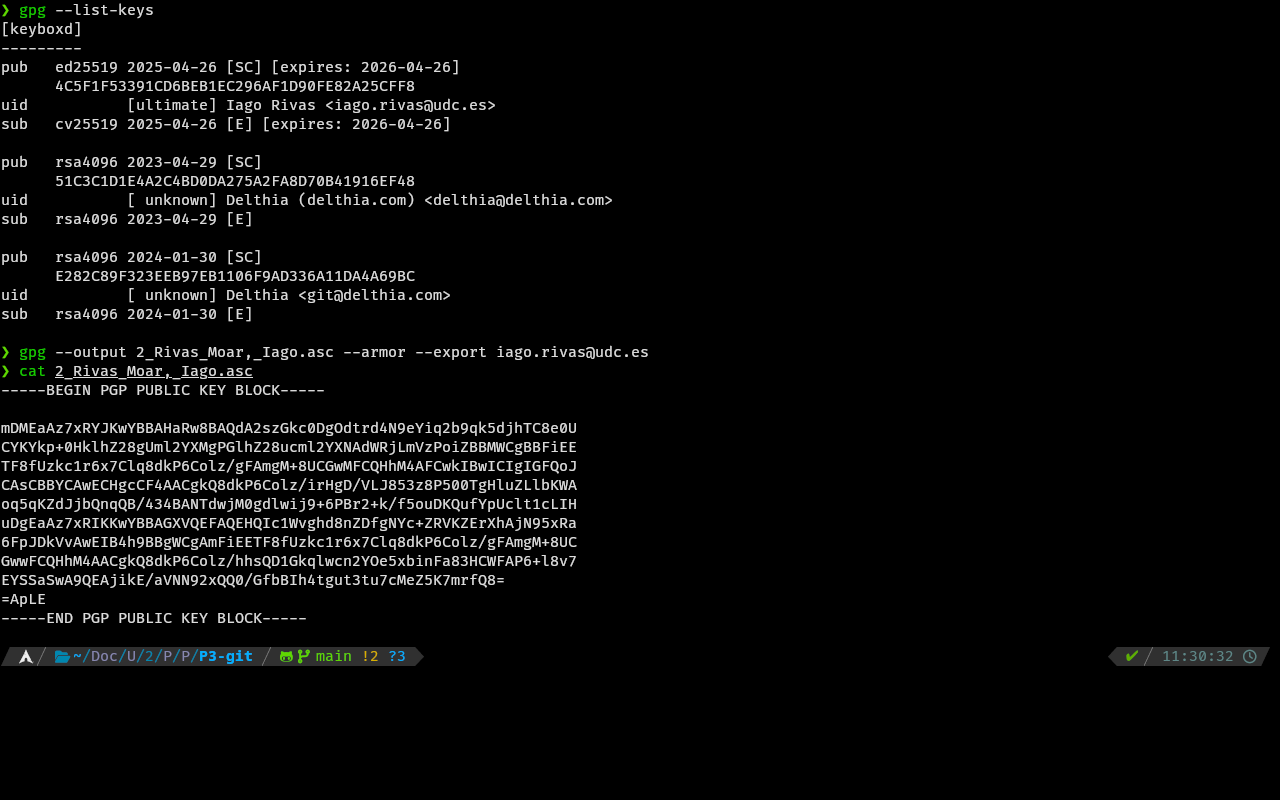
\includegraphics[width=\textwidth]{gpg-export.png}
    \caption{Exportación de la clave pública}
\end{figure}

Por último, si perdiéramos el control de nuestra clave privada y quisiéramos revocarla, utilizaríamos el comando

\begin{minted}[
    frame=single,
    framesep=8pt,
    breaklines,
    bgcolor=bgGray
]{bash}
    gpg --output iago.rivas-revocation.asc --armor --gen-revoke iago.rivas@udc.es
\end{minted}

Que generaría un comando de revocación que podríamos compartir a nuestros contactos.

\subsection{Ejercicio 7}
\graphicspath{ {img/07} }

Thunderbird es un lector de correo con un gran número de funcionalidades adicionales, como calendarios, contactos y, más importante en nuestro caso, permite utilizar PGP para cifrar y firmar los correos.

Para añadir las claves se utiliza la herramienta \texttt{Gestor de claves PGP}, donde se pueden importar tanto los pares de claves completos como solo las claves públicas, como se muestra a continuación:

\begin{figure}[H]
    \centering
    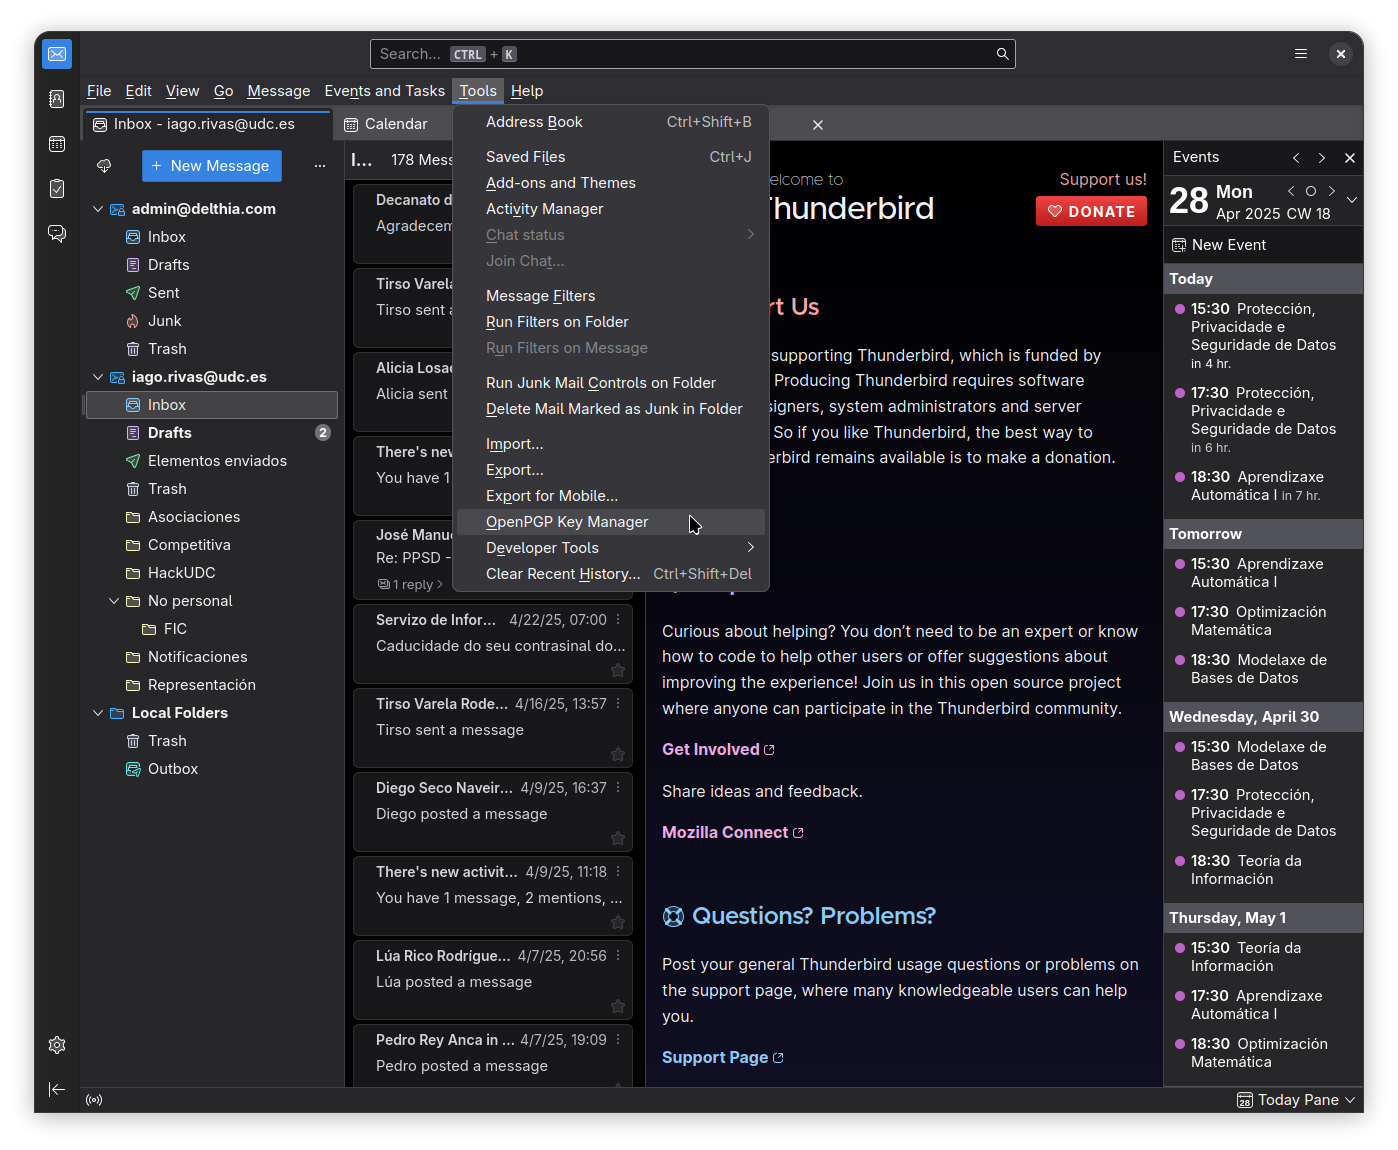
\includegraphics[width=\textwidth]{thunderbird-tools-menu.png}
    \caption{Menú con la herramienta “Gestión de claves OpenPGP”}
\end{figure}

\begin{figure}[H]
    \centering
    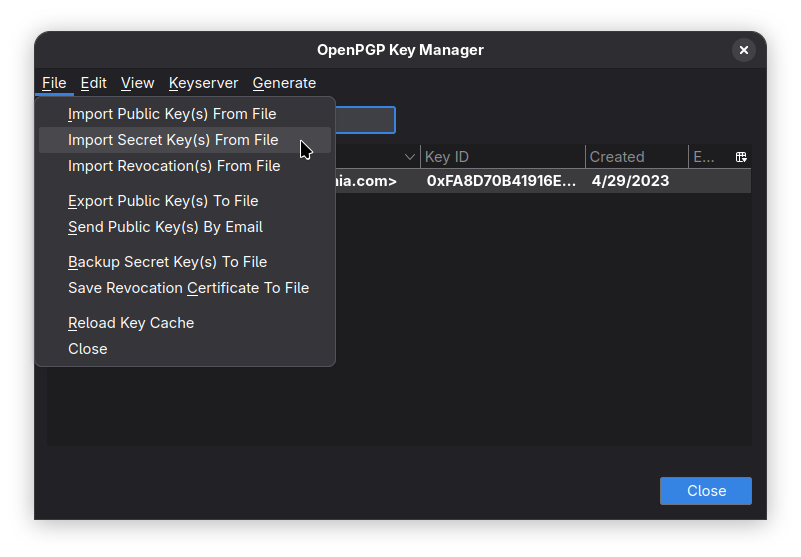
\includegraphics[width=10cm]{thunderbird-keymanager.png}
    \caption{Importación de claves en la herramienta “Gestión de claves OpenPGP”}
\end{figure}

\begin{figure}[H]
    \centering
    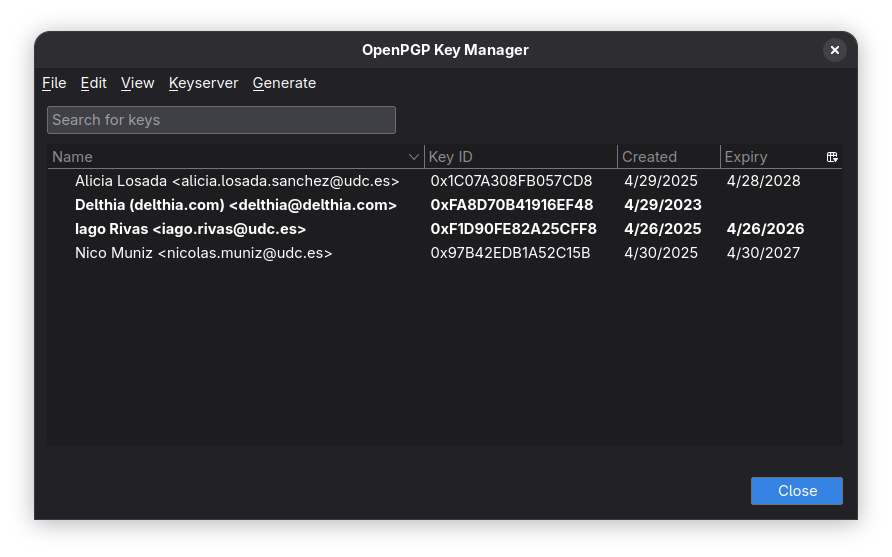
\includegraphics[width=10cm]{thunderbird-keymanager-keys.png}
    \caption{Claves PGP importadas en Thunderbird}
\end{figure}

Ahora, encriptar un correo es cuestión de selecciónar la opción “Encriptar” que se habilitará en la ventana de redacción, justo al lado del botón enviar. Junto a este botón hay un desplegable con tres opciones:
\begin{itemize}
    \item{\underline{Firmar:} Firma el correo con la clave del remitente. No afecta a la capacidad de leer el correo del destinatario.}
    \item{\underline{Encriptar:} Encripta el correo con la clave del destinatario, por lo que es necesario conoecer la clave pública del mismo. Además, el destinatario no podrá leer el correo sin desencriptarlo con su clave privada. Existe una opción que permite encriptar también el asunto.}
    \item{Firmar y encriptar: Primero se firma el correo y luego se encripta. Esto permite mantener la privacidad en la comunicación y que solo el destinatario, que puede leer el correo, pueda comprobar también que el remitente es quien dice ser.}
\end{itemize}

En estos casos el mensaje se envía como un bloque cifrado, y en caso de solo firmarse, se adjunta la firma. En otro lector de correo, por ejemplo la versión web de outlook, no podremos leer el mensaje y tendremos que descargarlo para desencriptarlo con \texttt{gpg}, mientras que Thunderbird muestra automáticamente los mensajes cifrados como si no lo estuvieran, además de indicar claramente si tienen una firma y si es válida.

En primer lugar se envió un correo firmado, luego un correo cifrado y, por último, un correo cifrado y firmado.

\begin{figure}[H]
    \centering
    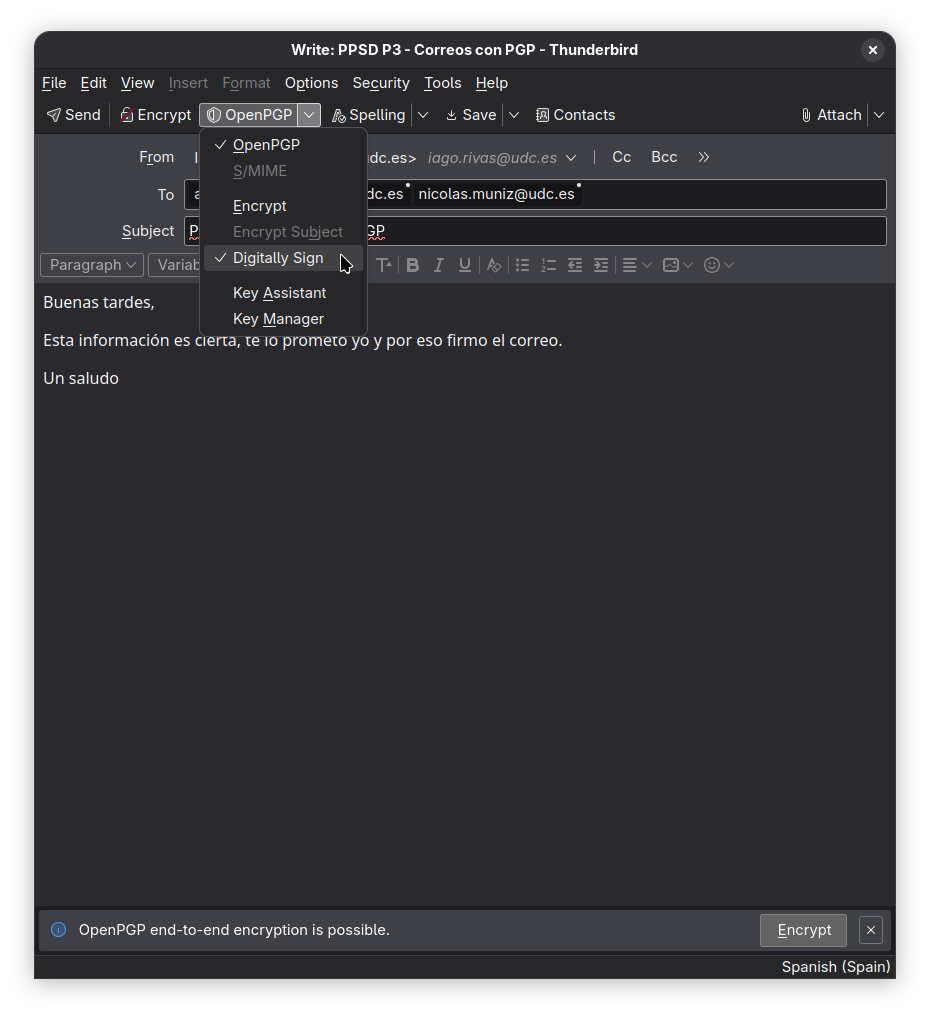
\includegraphics[width=10cm]{thunderbird-firmado.png}
    \caption{Envío de un correo firmado desde Thunderbird}
\end{figure}

\begin{figure}[H]
    \centering
    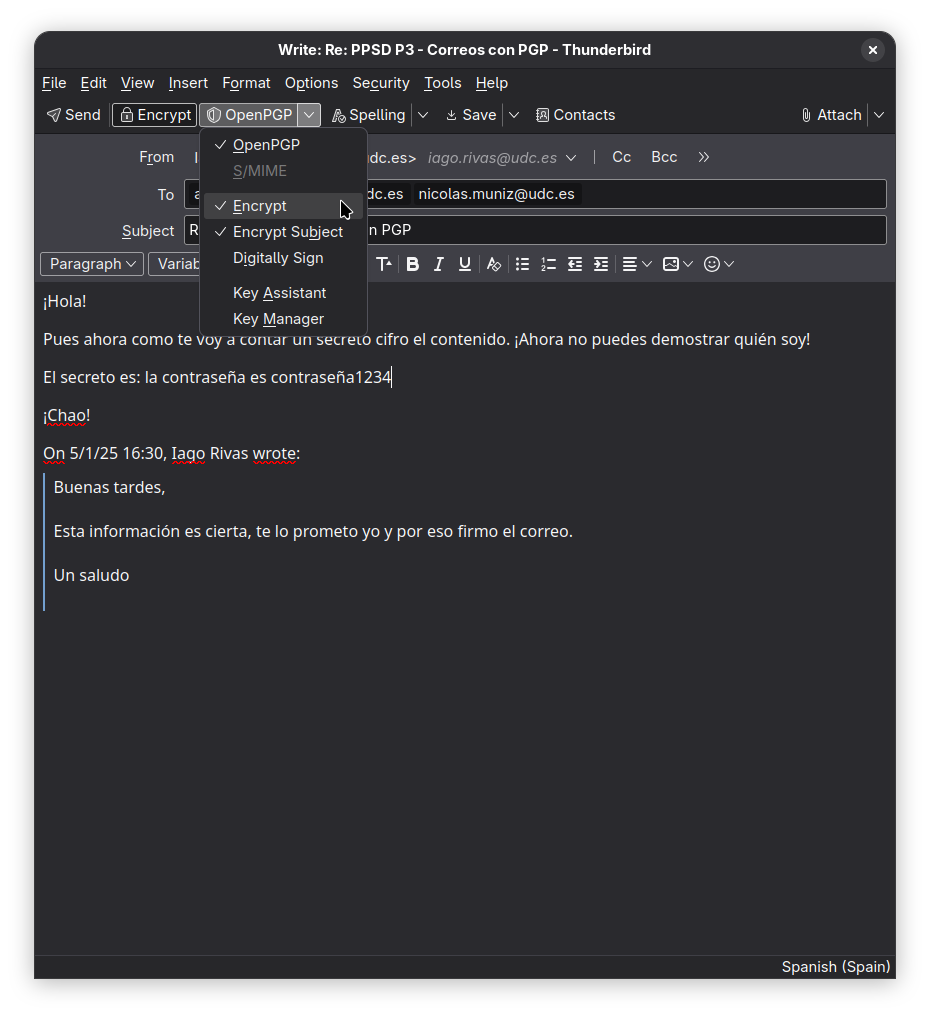
\includegraphics[width=10cm]{thunderbird-cifrado.png}
    \caption{Envío de un correo cifrado desde Thunderbird}
\end{figure}

\begin{figure}[H]
    \centering
    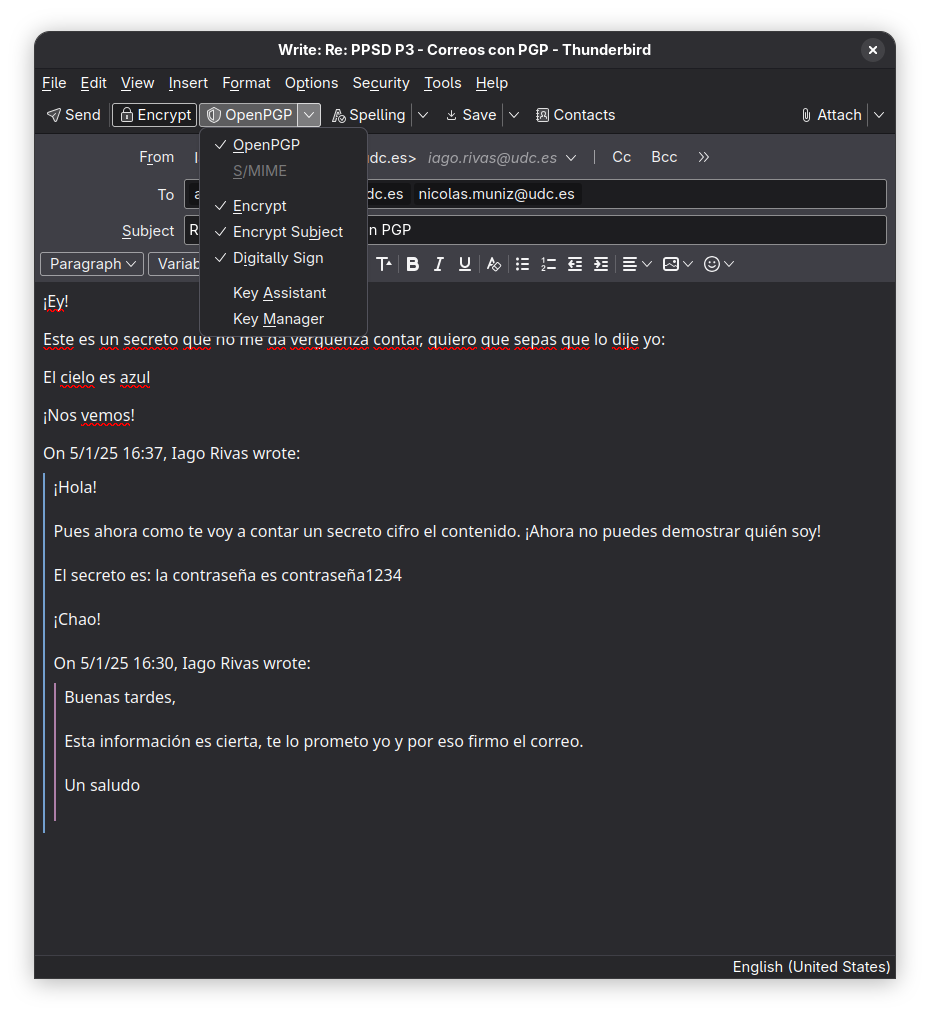
\includegraphics[width=10cm]{thunderbird-cifrado-firmado.png}
    \caption{Envío de un correo cifrado y firmado desde Thunderbird}
\end{figure}

\subsection{Ejercicio 8}

\subsection{Ejercicio 9}
\graphicspath{ {img/09} }

\subsubsection{Cifrado archivo}

Si queremos almacenar el archivo \texttt{secreto.txt} de manera segura, con OpenPGP, debemos cifrarlo con nuestra propia clave pública para que solo seamos nosotros, los únicos con acceso a nuestra clave privada, quienes podemos abrirlo. Además, al cifrar archivos para almacenarlos o compartirlos de otra manera, no necesitamos usar la \texttt{armor}, como hacíamos con el correo electrónico, ya que en este caso nos a igual que el archivo sea un archivo binario en bruto al no tener la limitación de ASCII del correo electrónico.

Así, para cifrar un archivo \texttt{secreto.txt} con PGP podemos usar el comando:

\begin{minted}[
    frame=single,
    framesep=8pt,
    breaklines,
    bgcolor=bgGray
]{bash}
    gpg --encrypt -r iago.rivas@udc.es secreto.txt
\end{minted}

\subsubsection{Cifrado correo electrónico}

La principal diferencia con los comandos utilizados para cifrar mensajes de correo electrónico es que no necesitamos almacenarlo en ASCII. Además, en este caso, como queremos cifrar el archivo para almacenarlo y necesitamos poder descifrarlo nosotros mismos en el futuro, nos pondremos como recipiente. Así, el archivo se cifra con nuestra propia clave pulica.

\subsubsection{Operaciones criptográficas en la operación}

Cuando se cifra un archivo con PGP usando la clave pública del destinatario, intervienen las siguientes operaciones criptográficas:
\begin{enumerate}
    \item \textbf{Comprensión del archivo}: el archivo se comprime (por ejemplo con ZIP), para reducir el tamaño y mejorar la eficiencia del cifrado.
    \item \textbf{Generación de una clave de sesión}: se genera una clave de sesión aleatoria, que se usará para cifrar el contenido del archivo de forma rápida y eficiente. Esta es una clave temporal válida solo para ese archivo o mensaje.
    \item \textbf{Cifrado simétrico del archivo comprimido con la clave de sesión}: el archivo comprimido se cifra con un algoritmo de cifrado simétrico (por ejemplo, AES o CAST5) usando la clave de sesión. Esto garantiza la confidencialidad del contenido.
    \item \textbf{Cifrado asimétrico de la clave de sesión con la clave pública del destinatario}: la clave de sesión se cifra con la clave pública del destinatario (por ejemplo, RSA). Esto asegura que solo el destinatario pueda recuperar la clave de sesión y, con ella, descifrar el archivo.
\end{enumerate}

La combinación de estas operaciones constituyen un cifrado híbrido que es característico del funcionamiento de PGP. Se usa cifrado simétrico para el contenido y cifrado asimétrico para proteger la clave de sesión.

\subsubsection{Cifrado simétrico}

Si, sin embargo, quisiéramos que el archivo se cifrara de manera simétrica (es decir, que se cifrara y descifrara con nuestra clave privada), simplemente tendríamos añadir la opción \texttt{--symmetric}, resultando el comando:

\begin{minted}[
    frame=single,
    framesep=8pt,
    breaklines,
    bgcolor=bgGray
]{bash}
    gpg --encrypt --symmetric -r iago.rivas@udc.es secreto.txt
\end{minted}

\subsection{Ejercicio 10}
\graphicspath{ {img/10} }

En la actualidad el certificado de persona física de la FNMT no permite su uso para cifrar conversaciones de correo electrónico. Como alternativa podemos generar nuestro propio certificado o utilizar uno de alguna CA reconocida. Decidimos generar nuestros propios certificados firmados por una CA también nuestra con \texttt{openssl}, ya que nos parecía la opción más didáctica.

\subsubsection{Generación de una CA con OpenSSL}

Para crear una CA necesitamos dos cosas, la clave con la que la CA firmara las peticiones de certificado y un certificado público para la CA del que los clientes se puedan fiar para validar los certificados que hayamos firmado.

Decidimos utilizar una clave RSA de 4096 bits. Con el siguiente comando generamos la clave privada de la misma y la almacenamos cifrada con DES:

\begin{minted}[
    frame=single,
    framesep=8pt,
    breaklines,
    bgcolor=bgGray
]{bash}
    openssl genrsa -des3 -out ca.key 4096
\end{minted}

Una vez generada la clave privada, necesitamos un certificado con la clave pública de la CA. Un formato común para compartir las claves públicas junto con su identidad es x509. Con esto, el certificado contiene información sobre la CA y la clave pública. La información puede ser variada, y algunos parámetros habituales son los que pide \texttt{openssl} de manera interactiva al generar el certificado

\begin{minted}[
    frame=single,
    framesep=8pt,
    breaklines,
    bgcolor=bgGray
]{bash}
    openssl req -new -x509 -days 1826 -key ca.key -out ca.crt
\end{minted}

Este comando genera el certificado en formato x509 para la clave \texttt{ca.key}. Indicamos que queremos que tenga una validez de 1826 días (5 años) y que se almacene en \texttt{ca.crt}.

Ahora tenemos una CA que podemos compartir con todos nuestros amigos para que añadan en sus ordenadores (si se fían de nosotros).

\subsubsection{Generación de certificados}

Con la CA en funcionamiento necesitamos generar certificados para nuestros usuarios. Esto tiene dos partes:

\begin{itemize}
    \item Generación de una petición de certificado por parte del usuario
    \item Generación de un certificado firmado por la CA
\end{itemize}

Es decir, igual que con la CA, el usuario genera una clave privada pero, en este caso, en lugar de generar su propio certificado de clave pública, genera con su parte privada una \textit{petición de certificado}. A continuación, la CA genera con esta información el certificado correspondiente. De esta forma, el usuario obtiene un certificado público firmado por la Autoridad Certificadora sin tener que compartir nunca su clave privada.

La clave privada del usuario será igual que la de la CA, RSA de 4096 cifrada con DES para su almacenamiento seguro, por lo que se puede generar con el mismo comando:

\begin{minted}[
    frame=single,
    framesep=8pt,
    breaklines,
    bgcolor=bgGray
]{bash}
    openssl genrsa -des3 -out iago.rivas.key 4096
\end{minted}

A continuación se genera la petición de certificado CSR \textit{Certificate Signing Request} con \texttt{openssl}

\begin{minted}[
    frame=single,
    framesep=8pt,
    breaklines,
    bgcolor=bgGray
]{bash}
    openssl req -new -key iago.rivas.key -out iago.rivas.csr
\end{minted}

Con esta petición, la autoridad puede firmar el certificado y devolvérselo al usuario para que lo comparta como su clave pulica. Esto se puede hacer con el siguiente comando en \texttt{openssl}:

\begin{minted}[
    frame=single,
    framesep=8pt,
    breaklines,
    bgcolor=bgGray
]{bash}
    openssl x509 -req -days 730 -in iago.rivas.csr -CA ca.crt -CAkey ca.key -set_serial 0xBEEF -out iago.rivas.crt -setalias "iago.rivas@udc.es" -addtrust emailProtection -addreject clientAuth -addreject serverAuth
\end{minted}

Todos los parámetros del certificado los definió el usuario al generar la petición, sin embargo hay algunas cosas que decide la CA, concretamente la duración del certificado, en este caso 730 días (2 años), el número de serie y las características del certificado, en este caso se permite su uso para el correo electrónico, pero se prohibe utilizarlo para cualquier tipo de autenticación.

Para generar el certificado es necesaria la clave privada de la CA, ya que se incluye la firma de la misma para darle validez ante aquellas personas que se fíen de la Autoridad pero no del usuario del certificado.

\subsubsection{S/MIME en Thunderbird}

Para utilizar nuestro certificado S/MIME en Thunderbird tenemos que añadir primero el certificado de la Autoirdad Certificadora y a continuación nuestro certificado. Necesitamos incluír la parte privada, ya que lo usaremos para firmar y descifrar mensajes, por lo que lo exportaremos en el formato PKCS12 también con openssl, utilizando el comando

\begin{minted}[
    frame=single,
    framesep=8pt,
    breaklines,
    bgcolor=bgGray
]{bash}
    openssl pkcs12 -export -in iago.rivas.crt -inkey iago.rivas.key -out iago.rivas.p12
\end{minted}

Ahora podemos firmar y cifrar mensajes del mismo modo que cuando utilizábamos OpenPGP, seleccionando en el mismo desplegable la opción de S/MIME, en lugar de OpenPGP.
\subsection{Ejercicio 11}

Comprobar la firma criptográfica de un paquete es realmente sencillo una vez que utilizamos \texttt{gpg} en los apartados anteriores. Lo primero es importar la clave pública del desarrollador, que como indica la propia web de \href{https://keepassxc.org/}{KeePassXC}, se puede descargar desde el keyserver \url{openpgp.org} con el comando

\begin{minted}[
    frame=single,
    framesep=8pt,
    breaklines,
    bgcolor=bgGray
]{bash}
    gpg --keyserver keys.openpgp.org --recv-keys BF5A669F2272CF4324C1FDA8CFB4C2166397D0D2
\end{minted}

Una vez descargado, podemos comprobar la firma del archivo con el comando

\begin{minted}[
    frame=single,
    framesep=8pt,
    breaklines,
    bgcolor=bgGray
]{bash}
    gpg --verify gpg --verify KeePassXC-2.7.10-x86_64.AppImage.sig
\end{minted}

de la misma forma que hacíamos con los correos electrónicos.

Si podemos asegurar que tenemos la clave pública adecuada una firma criptográfica es una manera mucho más segura de verificar que no se modificó el paquete, ya que el hash es una buena forma de comprobar la integridad que sería muy fácil de evadir en caso de querer servir un paquete comprometido, simplemente tendríamos que mostrar el hash correspondiente al paquete malicioso en la web. Con la firma esto es imposible si ya tenemos descargada la clave pública del desarrollador.

Tanto es así que los gestores de paquetes en GNU/Linux utilizan el método de la firma para verificar la integridad y la seguridad de los paquetes, ya que en esta situación, los paquetes se pueden descargar de diversos repositorios, llamados espejos que podrían gestionar diferentes personas o entidades. Así, todos los paquetes están firmados por el mantenedor de la distribución que estemos utilizando, asegurando que no se modificaron los paquetes independientemente del espejo que utilicemos, siempre que se valide la firma con la clave pública del mantenedor.

\section{Privacidad}
\subsection{Ejercicio 12}
\graphicspath{ {img/12} }

Los sitios web seleccionados fueron:
\begin{itemize}
    \item \url{www.wikipedia.org}
    \item \url{https://elpais.com/}
\end{itemize}

\subsubsection{Cookies almacenadas}

\begin{figure}[H]
    \centering
    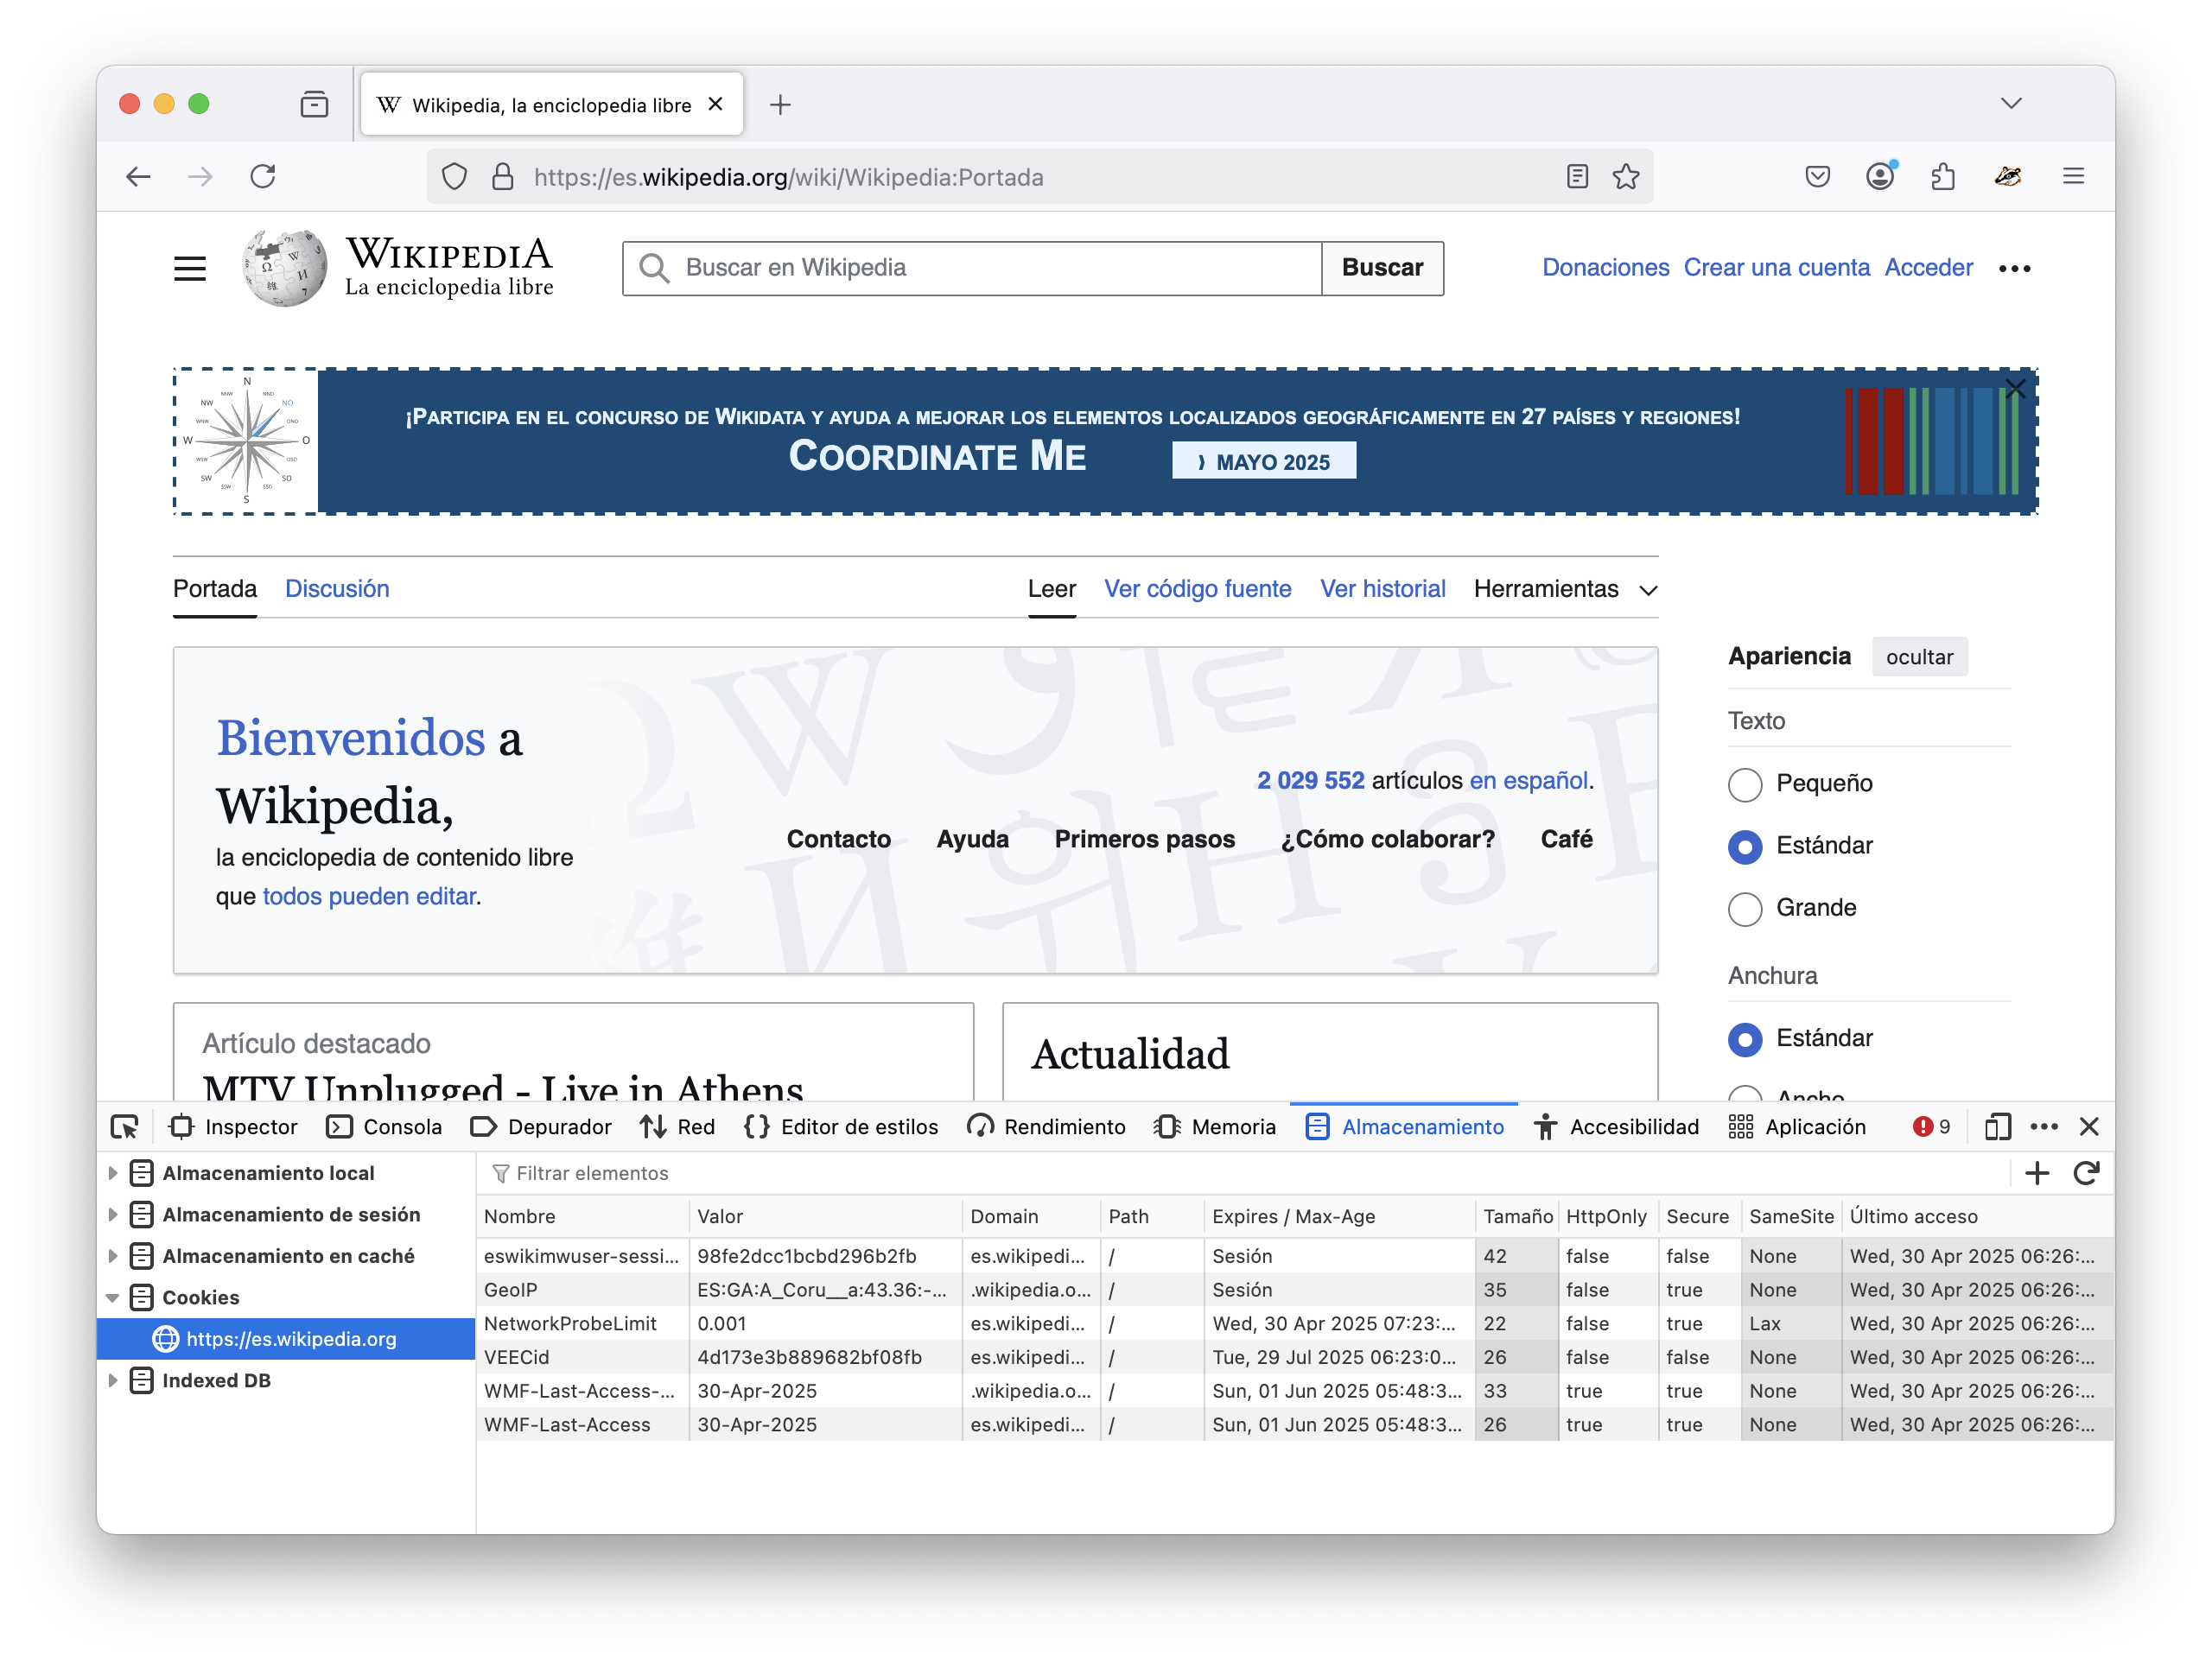
\includegraphics[width=\textwidth]{cookies_wiki.png}
    \caption{Cookies almacenadas por Wikipedia}
    \label{fig:cookies_wiki}
\end{figure}

El primer sitio web seleccionado es la Wikipedia. Para poder ver cuántas cookies se almacenan y cuáles son debemos inspeccionar la página. En \ref{fig:cookies_wiki} podemos ver cuáles son las cookies que se almacenan en el sitio web. Las 6 cookies almacenadas son: ``eswikiwmuser-sessionId'', ``GeoIP'', ``NetworkProbeLimit'', ``WMF-Last-Access'' (parece duplicada con distinto valor o ámbito de acceso) y ``centralnotice\_fundraising''.

Seleccionamos la cookie ``GeoIP'' para su análisis. Esta cookie contiene información sobre la localización del usuario (por ejemplo, país y región), y presenta los siguientes parámetros: 

\begin{itemize}
    \item \texttt{Expires (Sesión)}: se elimina al cerrar el navegador, lo que limita su persistencia.
    \item \texttt{HttpOnly (false)}: puede ser accedida mediante scripts JavaScript, lo cual implica un riesgo si hubiera un ataque de tipo XSS.  
    \item \texttt{Secure (false)}: puede transmitirse incluso si la conexión no es segura, aunque Wikipedia usa HTTPS por defecto.
    \item \texttt{SameSite (None)}: permite que esta cookie se envíe en peticiones entre sitios (cross-site), lo cual es potencialmente más vulnerable a ataques CSRF si no se combina con otras medidas.
\end{itemize}

Aunque la cookie no contiene datos especialmente sensibles, la combinación de ``Secure=false'', ``HttpOnly=false'' y ``SameSite=None'' la hace más vulnerable que otras cookies más restringidas. Sin embargo, dado que Wikipedia utiliza HTTPS obligatorio y no utiliza cookies de sesión crítica para usuarios no registrados, el riesgo real es bajo. 

\begin{figure}[H]   
    \centering
    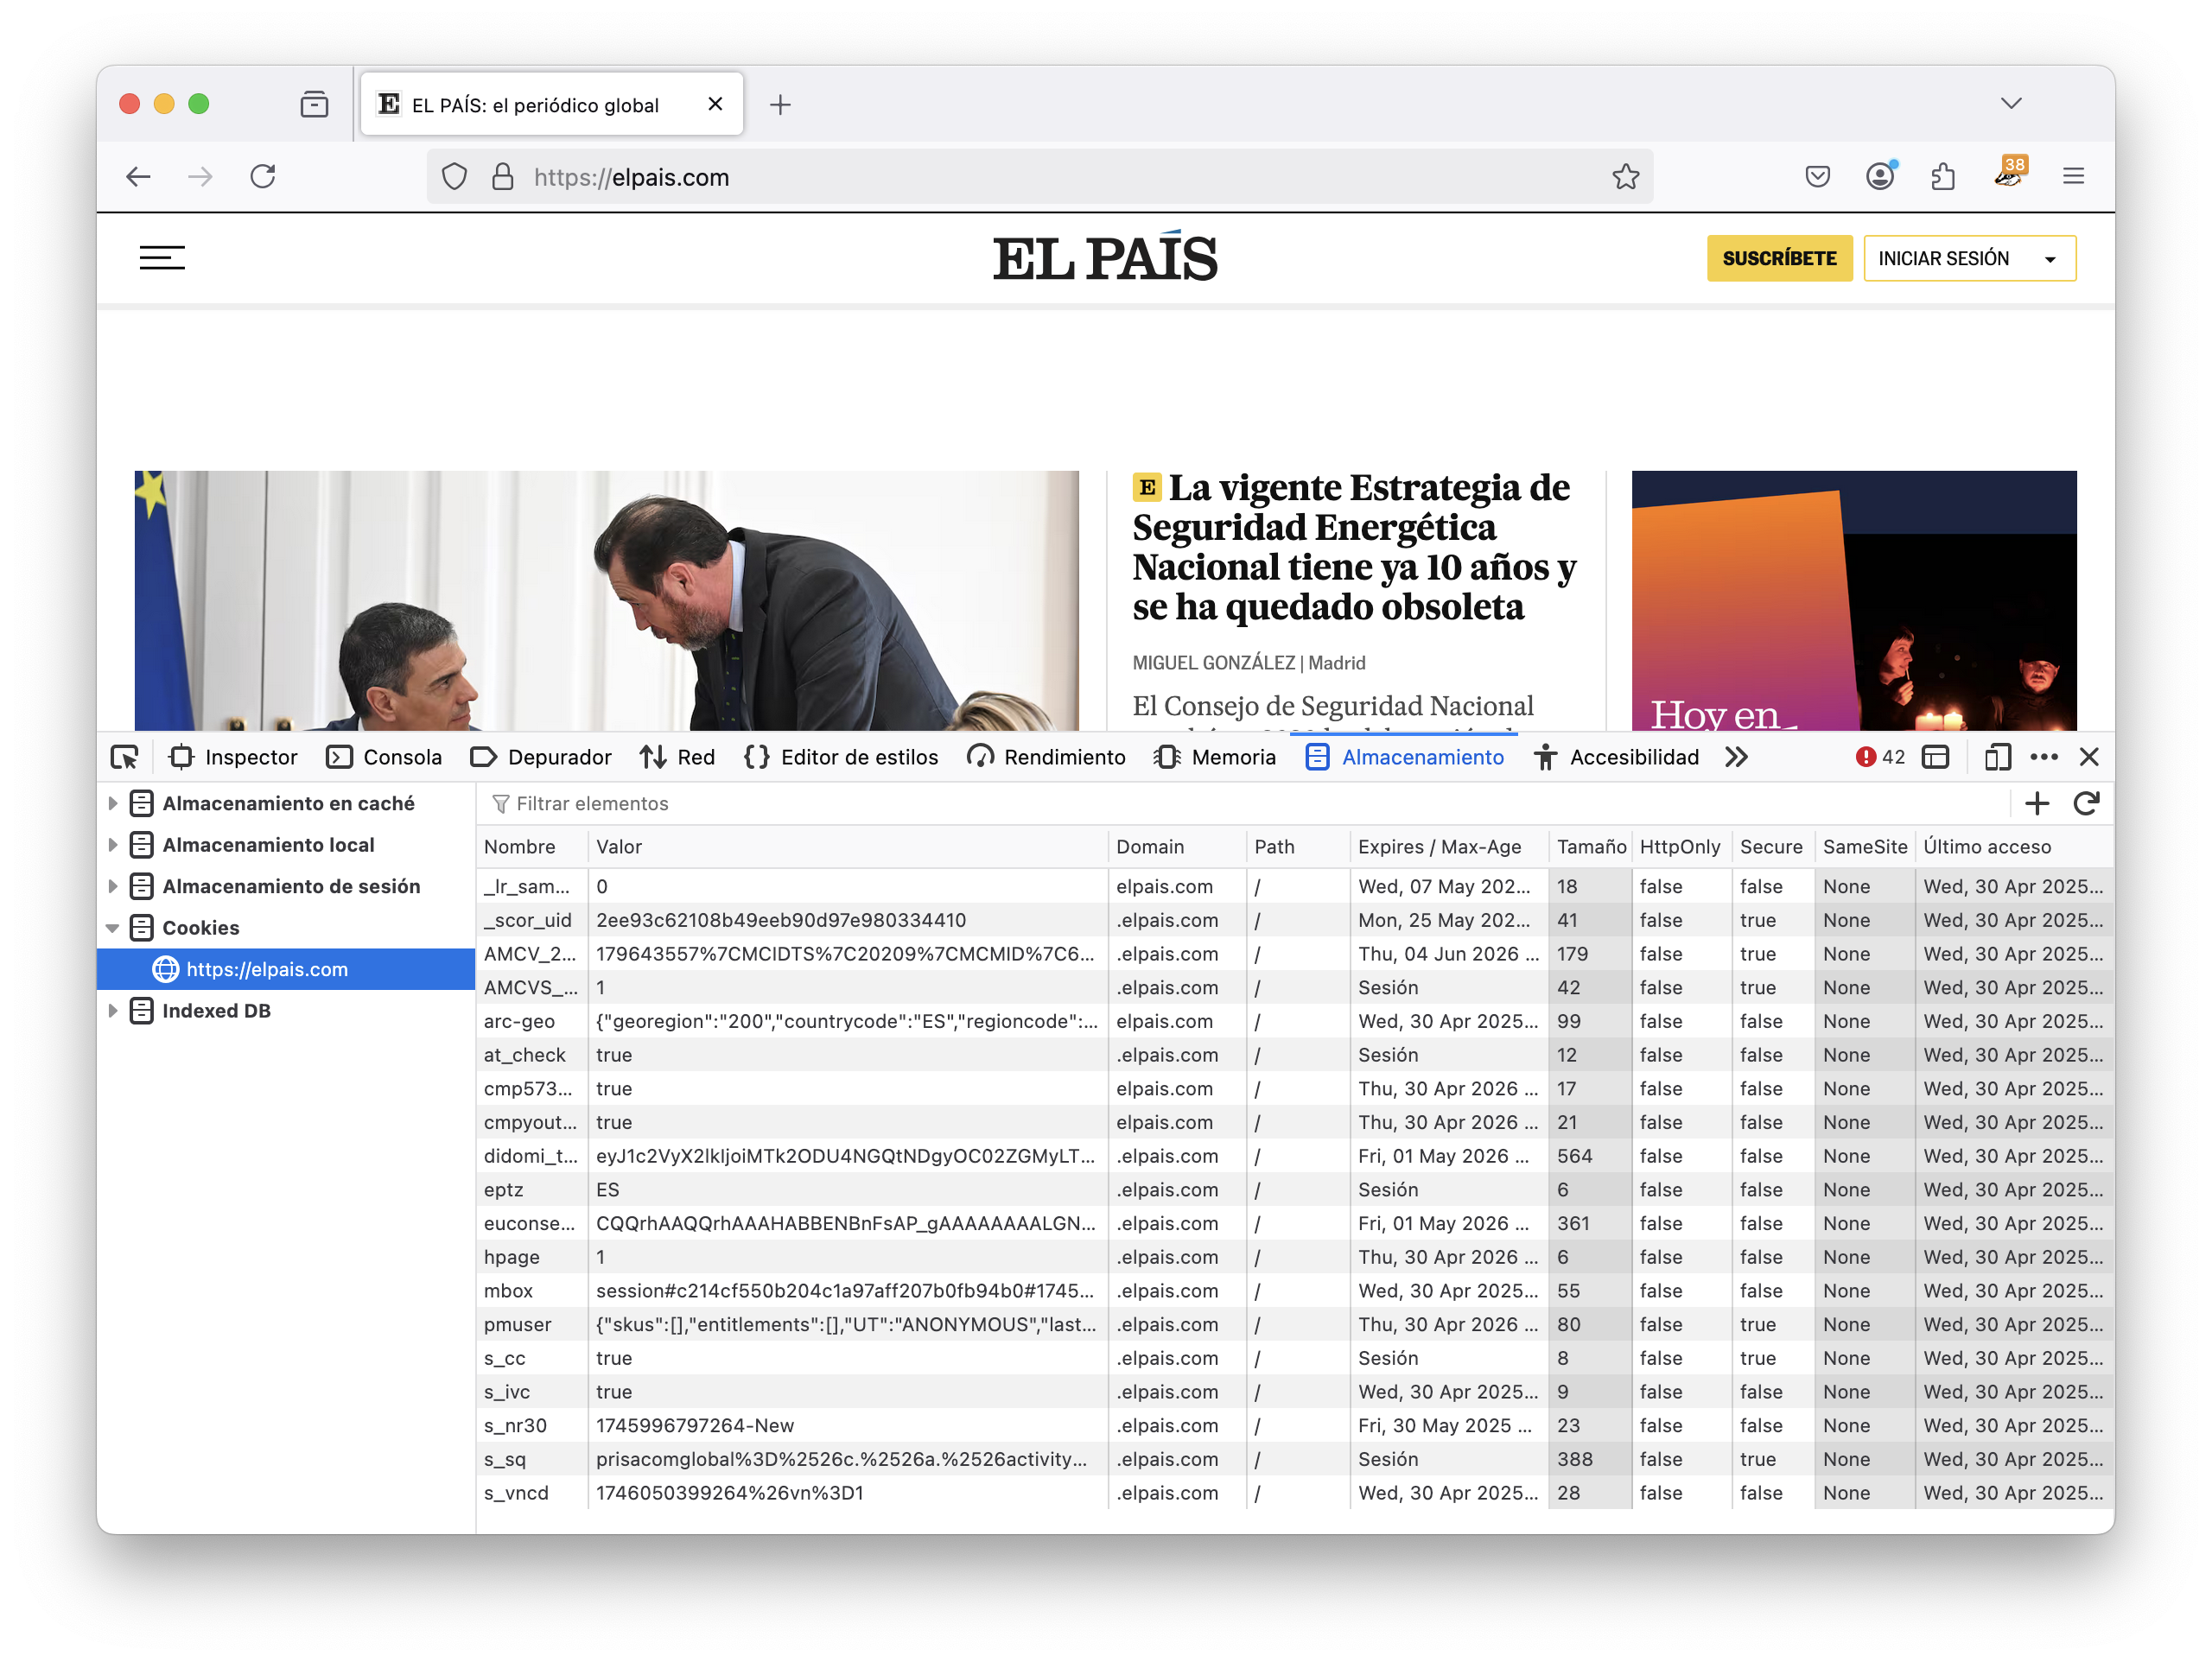
\includegraphics[width=\textwidth]{cookies_pais.png}
    \caption{Cookies almacenadas por El Pais}
    \label{fig:cookies_pais}
\end{figure}

El segundo sitio web seleccionado es El País. Tal y como hicimos con el dominio anterior, debemos inspeccionar la página. En \ref{fig:cookies_pais} podemos ver cuáles son las cookies que se almacenan en el sitio web. Se almacenan un total de 20 cookies distintas, todas ellas asociadas al mismo dominio, elpais.com.  

Seleccionamos la cookie ``AMCVS\_'' para su análisis. Esta cookie está relacionada con Adobe Analytics y se utiliza para identificar sesiones de usuario. Presenta los siguientes parámetros: 

\begin{itemize}
    \item \texttt{Expires (Sesión)}: se elimina al cerrar el navegador, lo que limita su persistencia.
    \item \texttt{HttpOnly (false)}: puede ser accedida mediante scripts JavaScript, lo cual implica un riesgo si hubiera un ataque de tipo XSS.  
    \item \texttt{Secure (true)}: solo se transmite a través de conexiones HTTPS, lo cual mejora su seguridad.
    \item \texttt{SameSite (None)}: permite que esta cookie se envíe en peticiones entre sitios (cross-site), lo cual es potencialmente más vulnerable a ataques CSRF si no se combina con otras medidas.
\end{itemize}

Aunque la cookie no contiene información directamente sensible, el hecho de que sea accesible desde JavaScript (HttpOnly=false) y pueda ser enviada entre sitios (SameSite=None) la hace más expuesta a ciertos ataques, especialmente si el sitio web tiene fallos de seguridad no corregidos. No obstante, al estar marcada como Secure, su transmisión está protegida frente a interceptación en redes no cifradas. 

\subsubsection{Cookies persistentes y de sesión}

Para determinar si las cookies almacenadas en ambos dominios web, debemos analizar el campo ``Expires/Max-Age''. En función de su persistencia, podemos dividir las cookies en dos grupos: persistentes y de sesión. Las cookies persistentes tienen fecha de expiración futura, lo que significa que se guardan incluso después de cerrar el navegador. Al contrario que las anteriores, las cookies de sesión se eliminan al cerrar el navegador. Se identifican fácilmente, pues en el campo mencionado toman el valor ``Sesión''. 

En el caso de la Wikipedia, las cookies persistentes son: ``NetworkProbeLimit'' (expira el 30 de abril de 2025), ``WMF-Last-Access 1'' (expira el 29 de julio de 2025), ``WMF-Last-Access 2'' (expira el 1 de junio de 2025) y ``centralnotice\_fundraising'' (expira el 1 de junio de 2025). Las cookies que se borrarán al cerrar el navegador son: ``eswikiwmuser-sessionId'' y ``GeoIP''.

En el caso de El País, de entre sus 20 cookies distintas, las que se borrarán al cerrar el navegador son: ``AMCVS\_'', ``arc-check'', ``ept2'' y ``sessionfc''. Las 16 cookies restantes son persistentes, ya que muestran fechas de caducidad. El rango de expiración de las cookies persistentes en elpais.com va desde el 30 de abril de 2025 hasta el 4 de agosto de 2026, lo que indica que algunas cookies están pensadas para mantenerse activas durante más de un año, especialmente aquellas vinculadas a analítica o personalización del usuario. 

\subsubsection{Cookies de terceros}

Como se ve en \ref{fig:cookies_wiki}, en el momento de la visita a Wikipedia, no se almacenaron cookies de terceros. Todas las cookies visibles pertenecen al dominio principal es.wikipedia.org, lo cual es coherente con la política de privacidad de Wikipedia, que no utiliza rastreadores ni servicios publicitarios externos en su página principal. 

Por otra parte, como se ve en \ref{fig:cookies_pais}, en el momento de la visita a El País, se observa que todas las cookies están asociadas al dominio elpais.com, por lo que se consideran cookies de primera parte. No obstante, es posible que se carguen cookies de terceros más adelante, si se acepta el uso de publicidad personalizada o se navega más profundamente por el sitio.

\subsubsection{Cookies eliminadas y navegación privada}

Para eliminar todas las cookies de ambos sitios web, debemos hacer click derecho en cualquiera de las cookies que se ven en \ref{fig:cookies_wiki} y \ref{fig:cookies_pais}, y seleccionamos la opción ``Eliminar todo de `es.wikipedia.org' '' en el caso de Wikipedia y ``Eliminar todo de `elpais.com' ''. Una vez hecho esto, procedimos a acceder a ambas webs en modo navegación privada. 

\begin{figure}[H]   
    \centering
    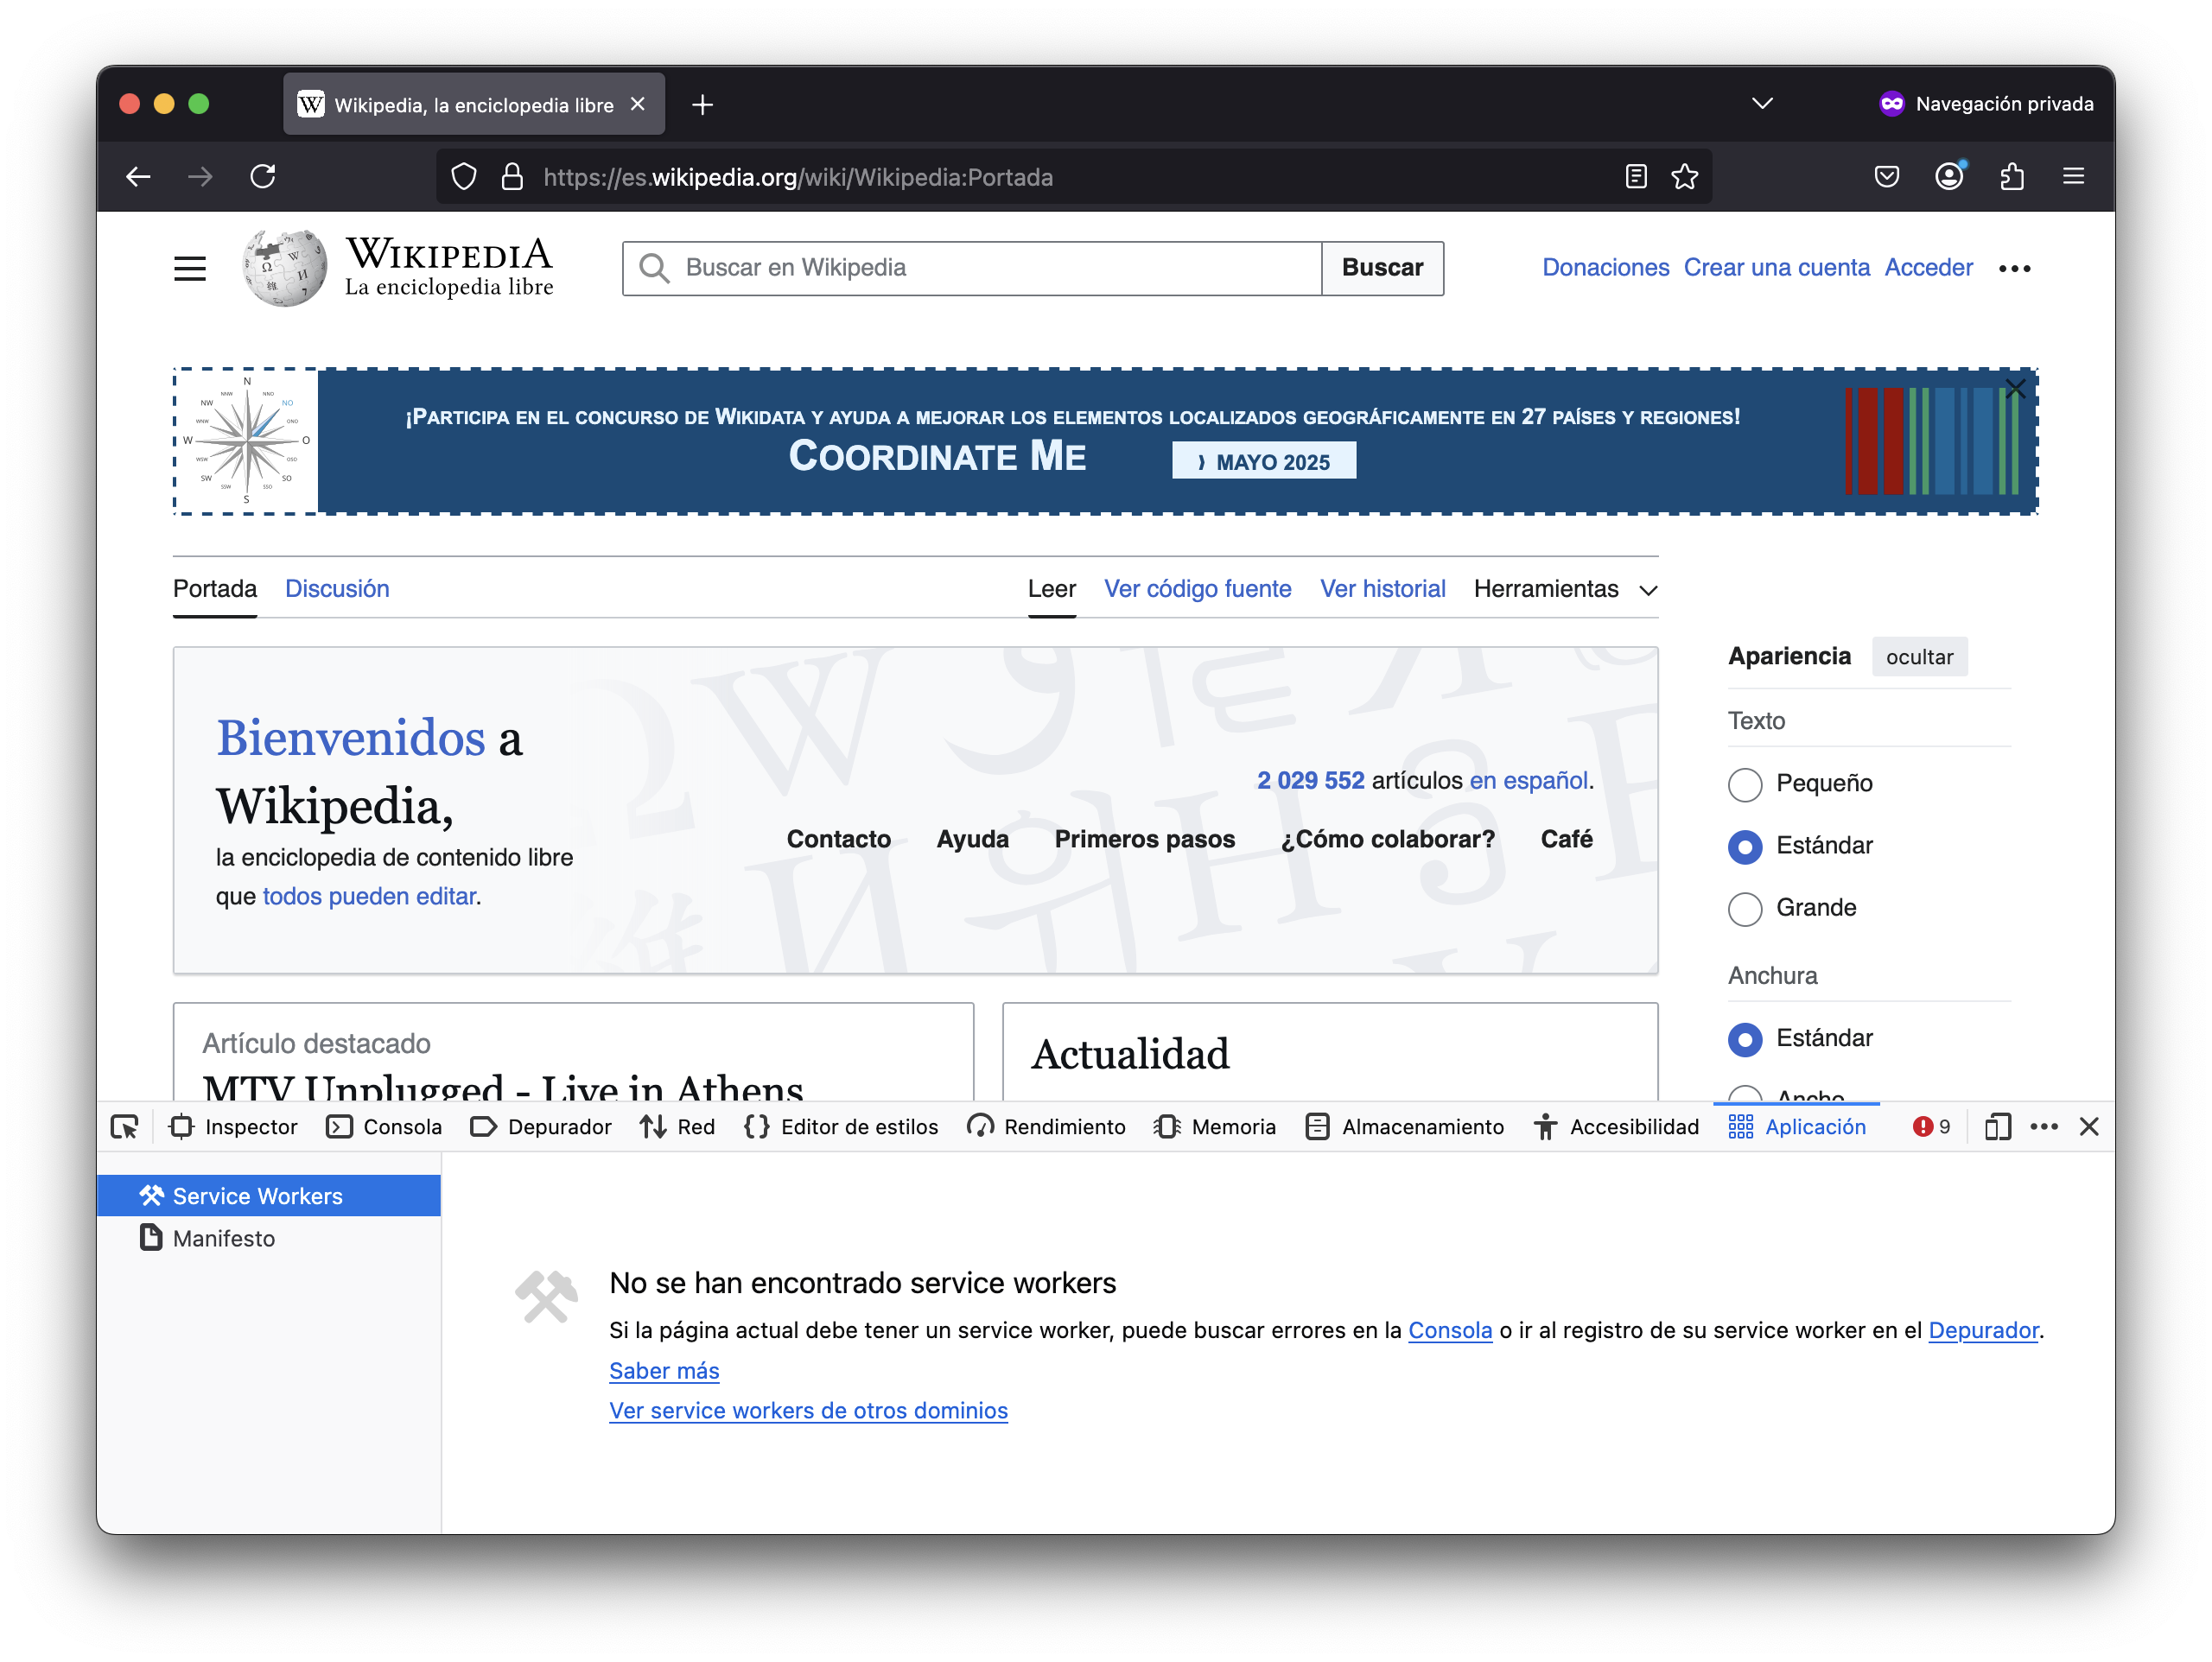
\includegraphics[width=\textwidth]{cookies_wiki_npriv.png}
    \caption{Cookies almacenadas por Wikipedia en navegación privada tras eliminación}
    \label{fig:cookies_wiki_npriv}
\end{figure}

Al eliminar todas las cookies del sitio wikipedia.org, se borra toda la información previamente almacenada, incluyendo identificadores de sesión, preferencias de idioma o geolocalización (por ejemplo, cookies como GeoIP o WMF-Last-Access). Sin embargo, la navegación por el sitio no se ve afectada, ya que Wikipedia no depende de cookies para su funcionamiento básico, especialmente si el usuario no ha iniciado sesión. 

Al acceder a Wikipedia en modo de navegación privada, se comprueba, como se muestra en \ref{fig:cookies_wiki_npriv}, que no se han generado cookies persistentes ni otros datos de almacenamiento, como service workers o bases de datos. Esto es coherente con el comportamiento de Wikipedia, que aplica una política de privacidad estricta: no utiliza rastreadores ni cookies de terceros, y solo crea cookies mínimas y temporales necesarias para aspectos técnicos. Además, al cerrar la ventana privada, cualquier cookie temporal generada durante la sesión se elimina automáticamente, dejando el navegador sin rastro de la actividad. 

\begin{figure}[H]   
    \centering
    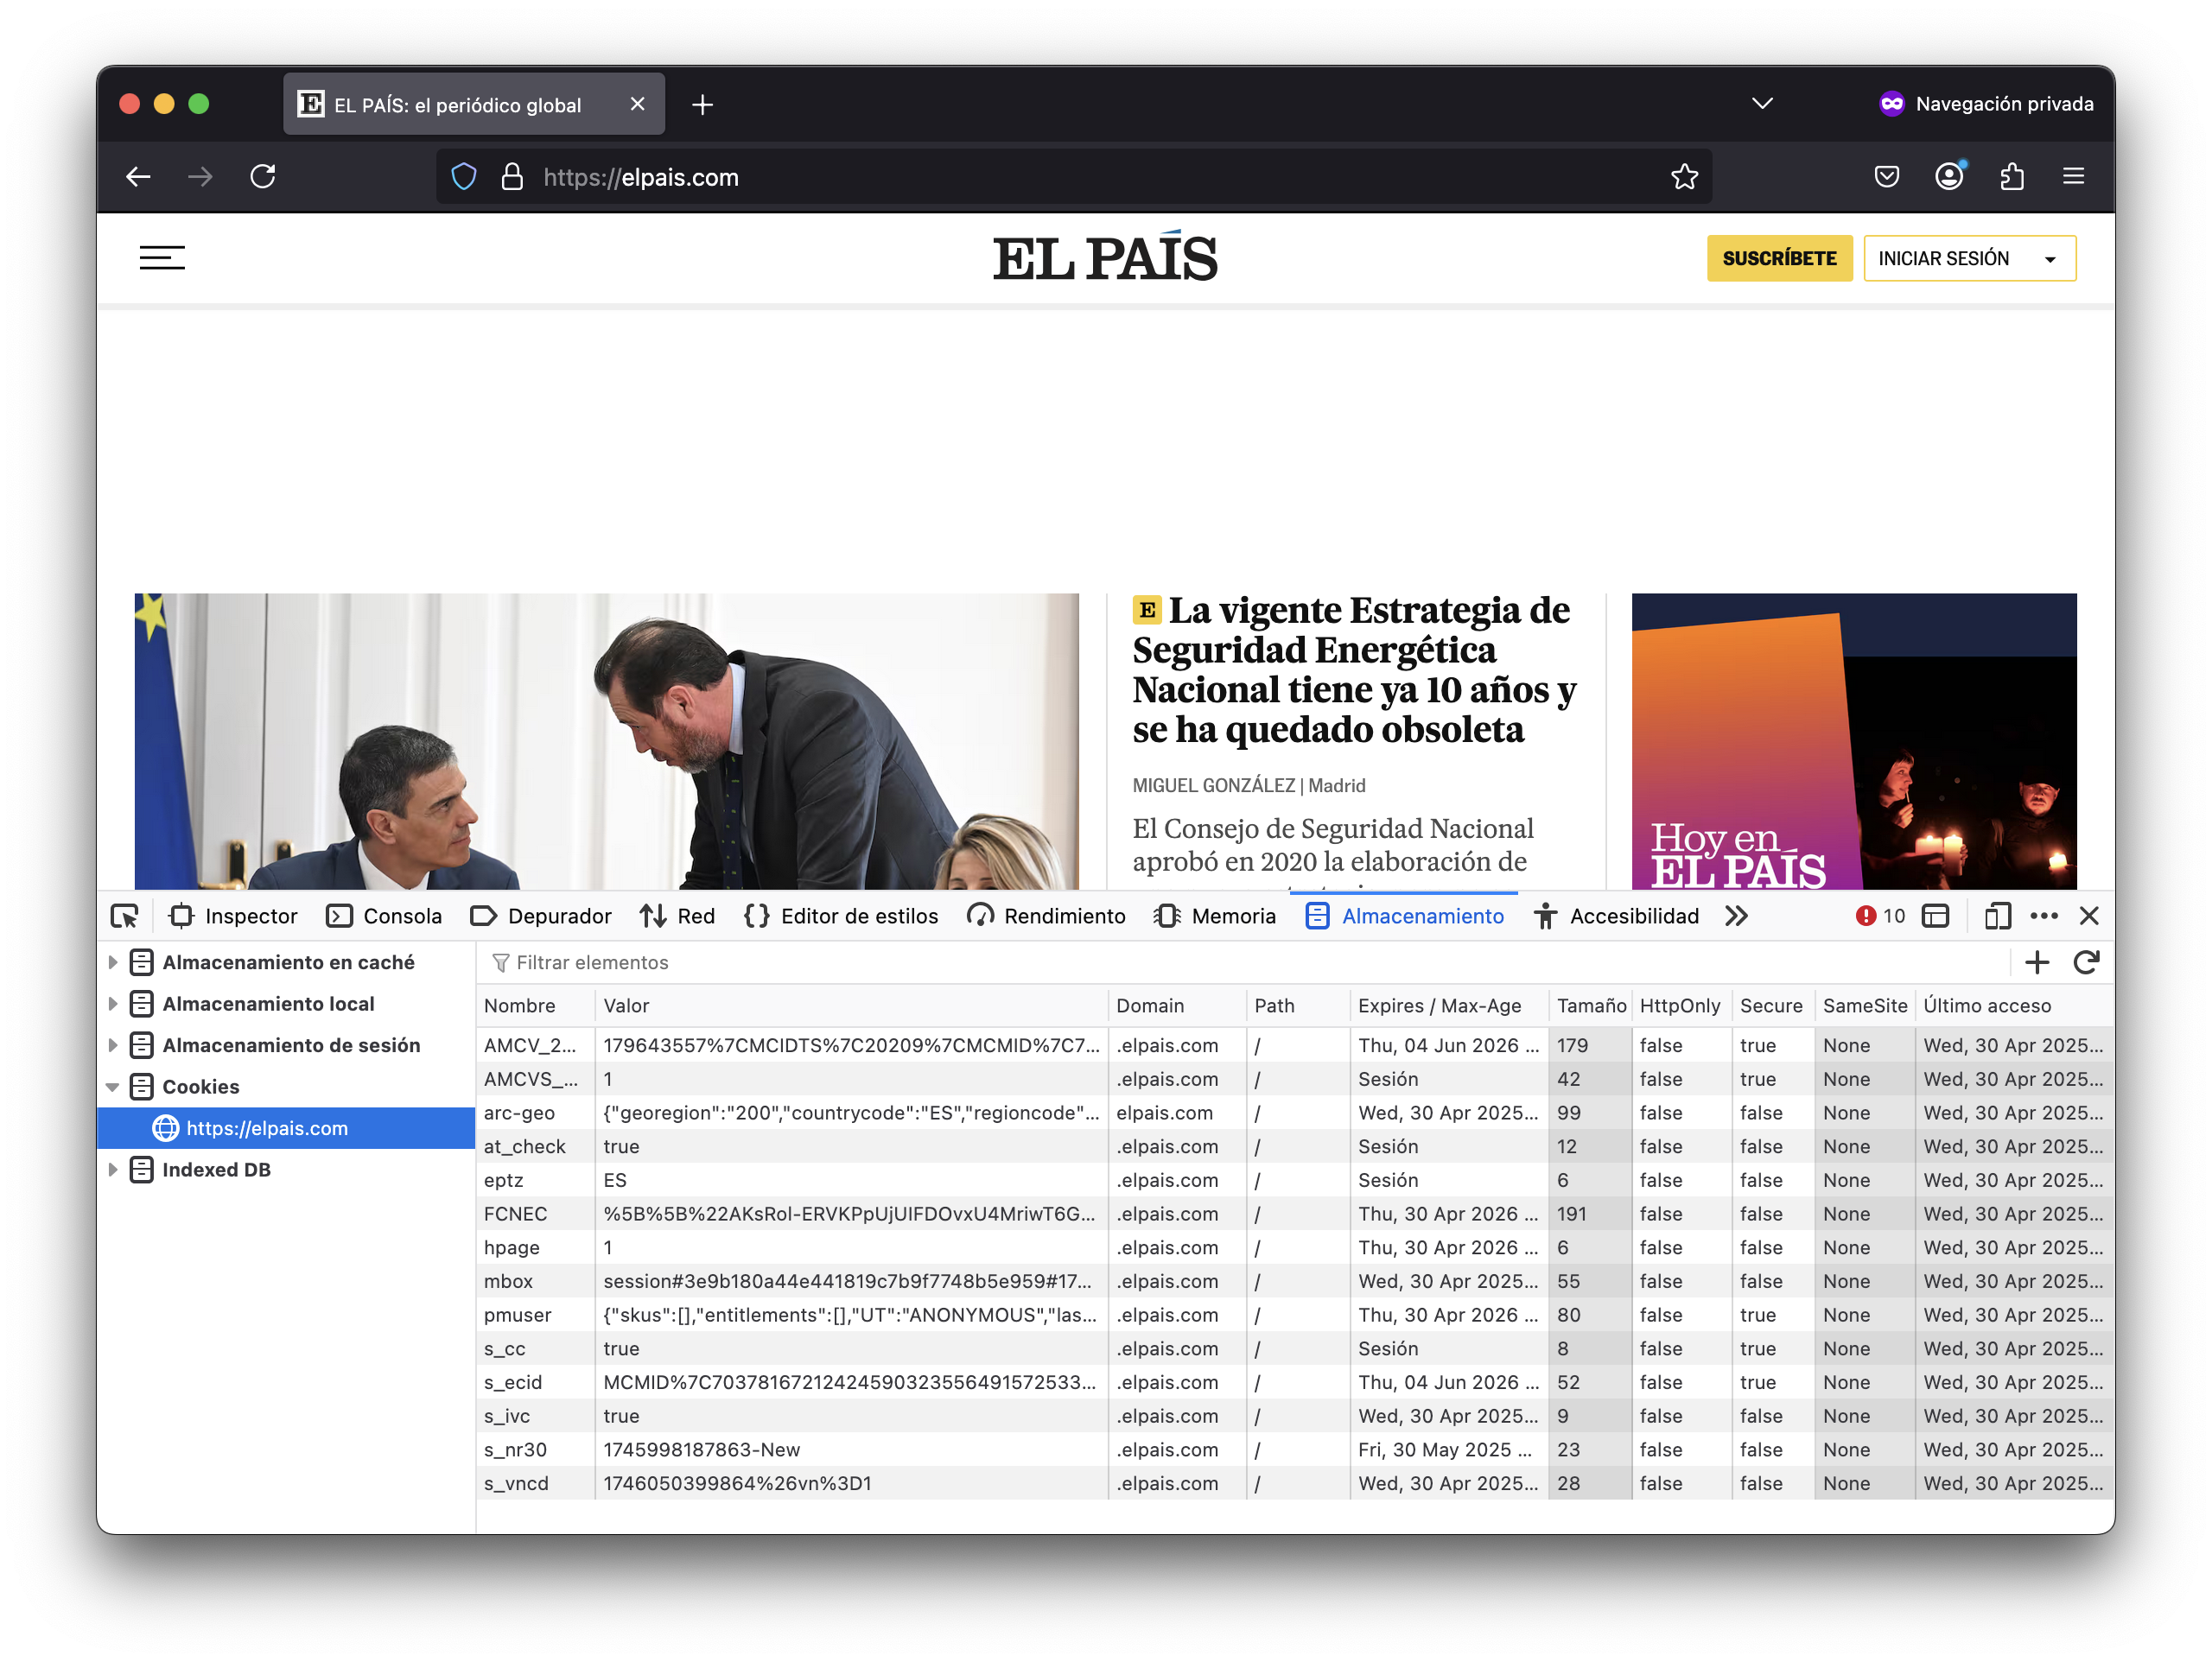
\includegraphics[width=\textwidth]{cookies_pais_npriv.png}
    \caption{Cookies almacenadas en El País en navegación privada tras eliminación}
    \label{fig:cookies_pais_npriv}
\end{figure}

Al eliminar todas las cookies del sitio elpais.com, se pierde la información relacionada con la sesión, el consentimiento de cookies y otros datos de navegación. Al volver a visitar la página, se muestra nuevamente el aviso de consentimiento, y el sitio crea nuevas cookies mínimas para gestionar la sesión. La navegación no se ve interrumpida, pero se reinicia el seguimiento y es necesario volver a aceptar (o rechazar) las cookies para personalizar la experiencia. 

Tras acceder en modo de navegación privada, como se ve en \ref{fig:cookies_pais_npriv}, el sitio vuelve a generar varias cookies, como AMCVS\_, arc\_geo, mbox, s\_cc, entre otras. Estas cookies permiten el funcionamiento del sitio y ciertos servicios de analítica, pero todas ellas son temporales: al cerrar la ventana privada, se eliminarán automáticamente, sin quedar rastro en el navegador. Esto confirma que El País, aunque instala cookies al cargar, no mantiene ninguna persistente tras finalizar la sesión privada, cumpliendo el comportamiento esperado del modo incógnito. 

\subsection{Ejercicio 13}

\subsection{Ejercicio 14}
\graphicspath{ {img/4} }

\begin{itemize}
    \item \href{https://support.mozilla.org/es/kb/Gestionar-la-configuraci%C3%B3n-del-almacenamiento-local-del-sitio?as=u&utm_source=inproduct&redirectslug=permission-store-data&redirectlocale=en-US}{support.mozilla.org}
    \item \href{https://librewolf.net/docs/faq/#how-do-i-stay-logged-into-specific-websites}{support.librewolf.org}
    \item \href{https://addons.mozilla.org/en-US/firefox/addon/cookie-autodelete/}{cookie_autodelete.org}
    \item \href{https://privacybadger.org/}{privacybadger.org}
\end{itemize}


\subsubsection{Configuración cookies Mozilla Firefox}

El navegador Mozilla Firefox proporciona múltiples opciones relacionadas con la gestión de cookies [support.mozilla.org]. Entre ellos, se destacan: 

\paragraph{Acceder a los ajustes de almacenamiento del sitio }

Esta opción permite ver y gestionar qué datos (cookies y caché) guarda cada sitio web en el navegador. Para ello, el usuario debe acceder al apartado de preferencias dentro del menú de Firefox. Una vez ahí, como se ve en la \ref{fig: opcion1_ej14} en el apartado de privacidad y seguridad se puede ver información acerca de las cookies del sitio. 

\begin{figure}[H]   
    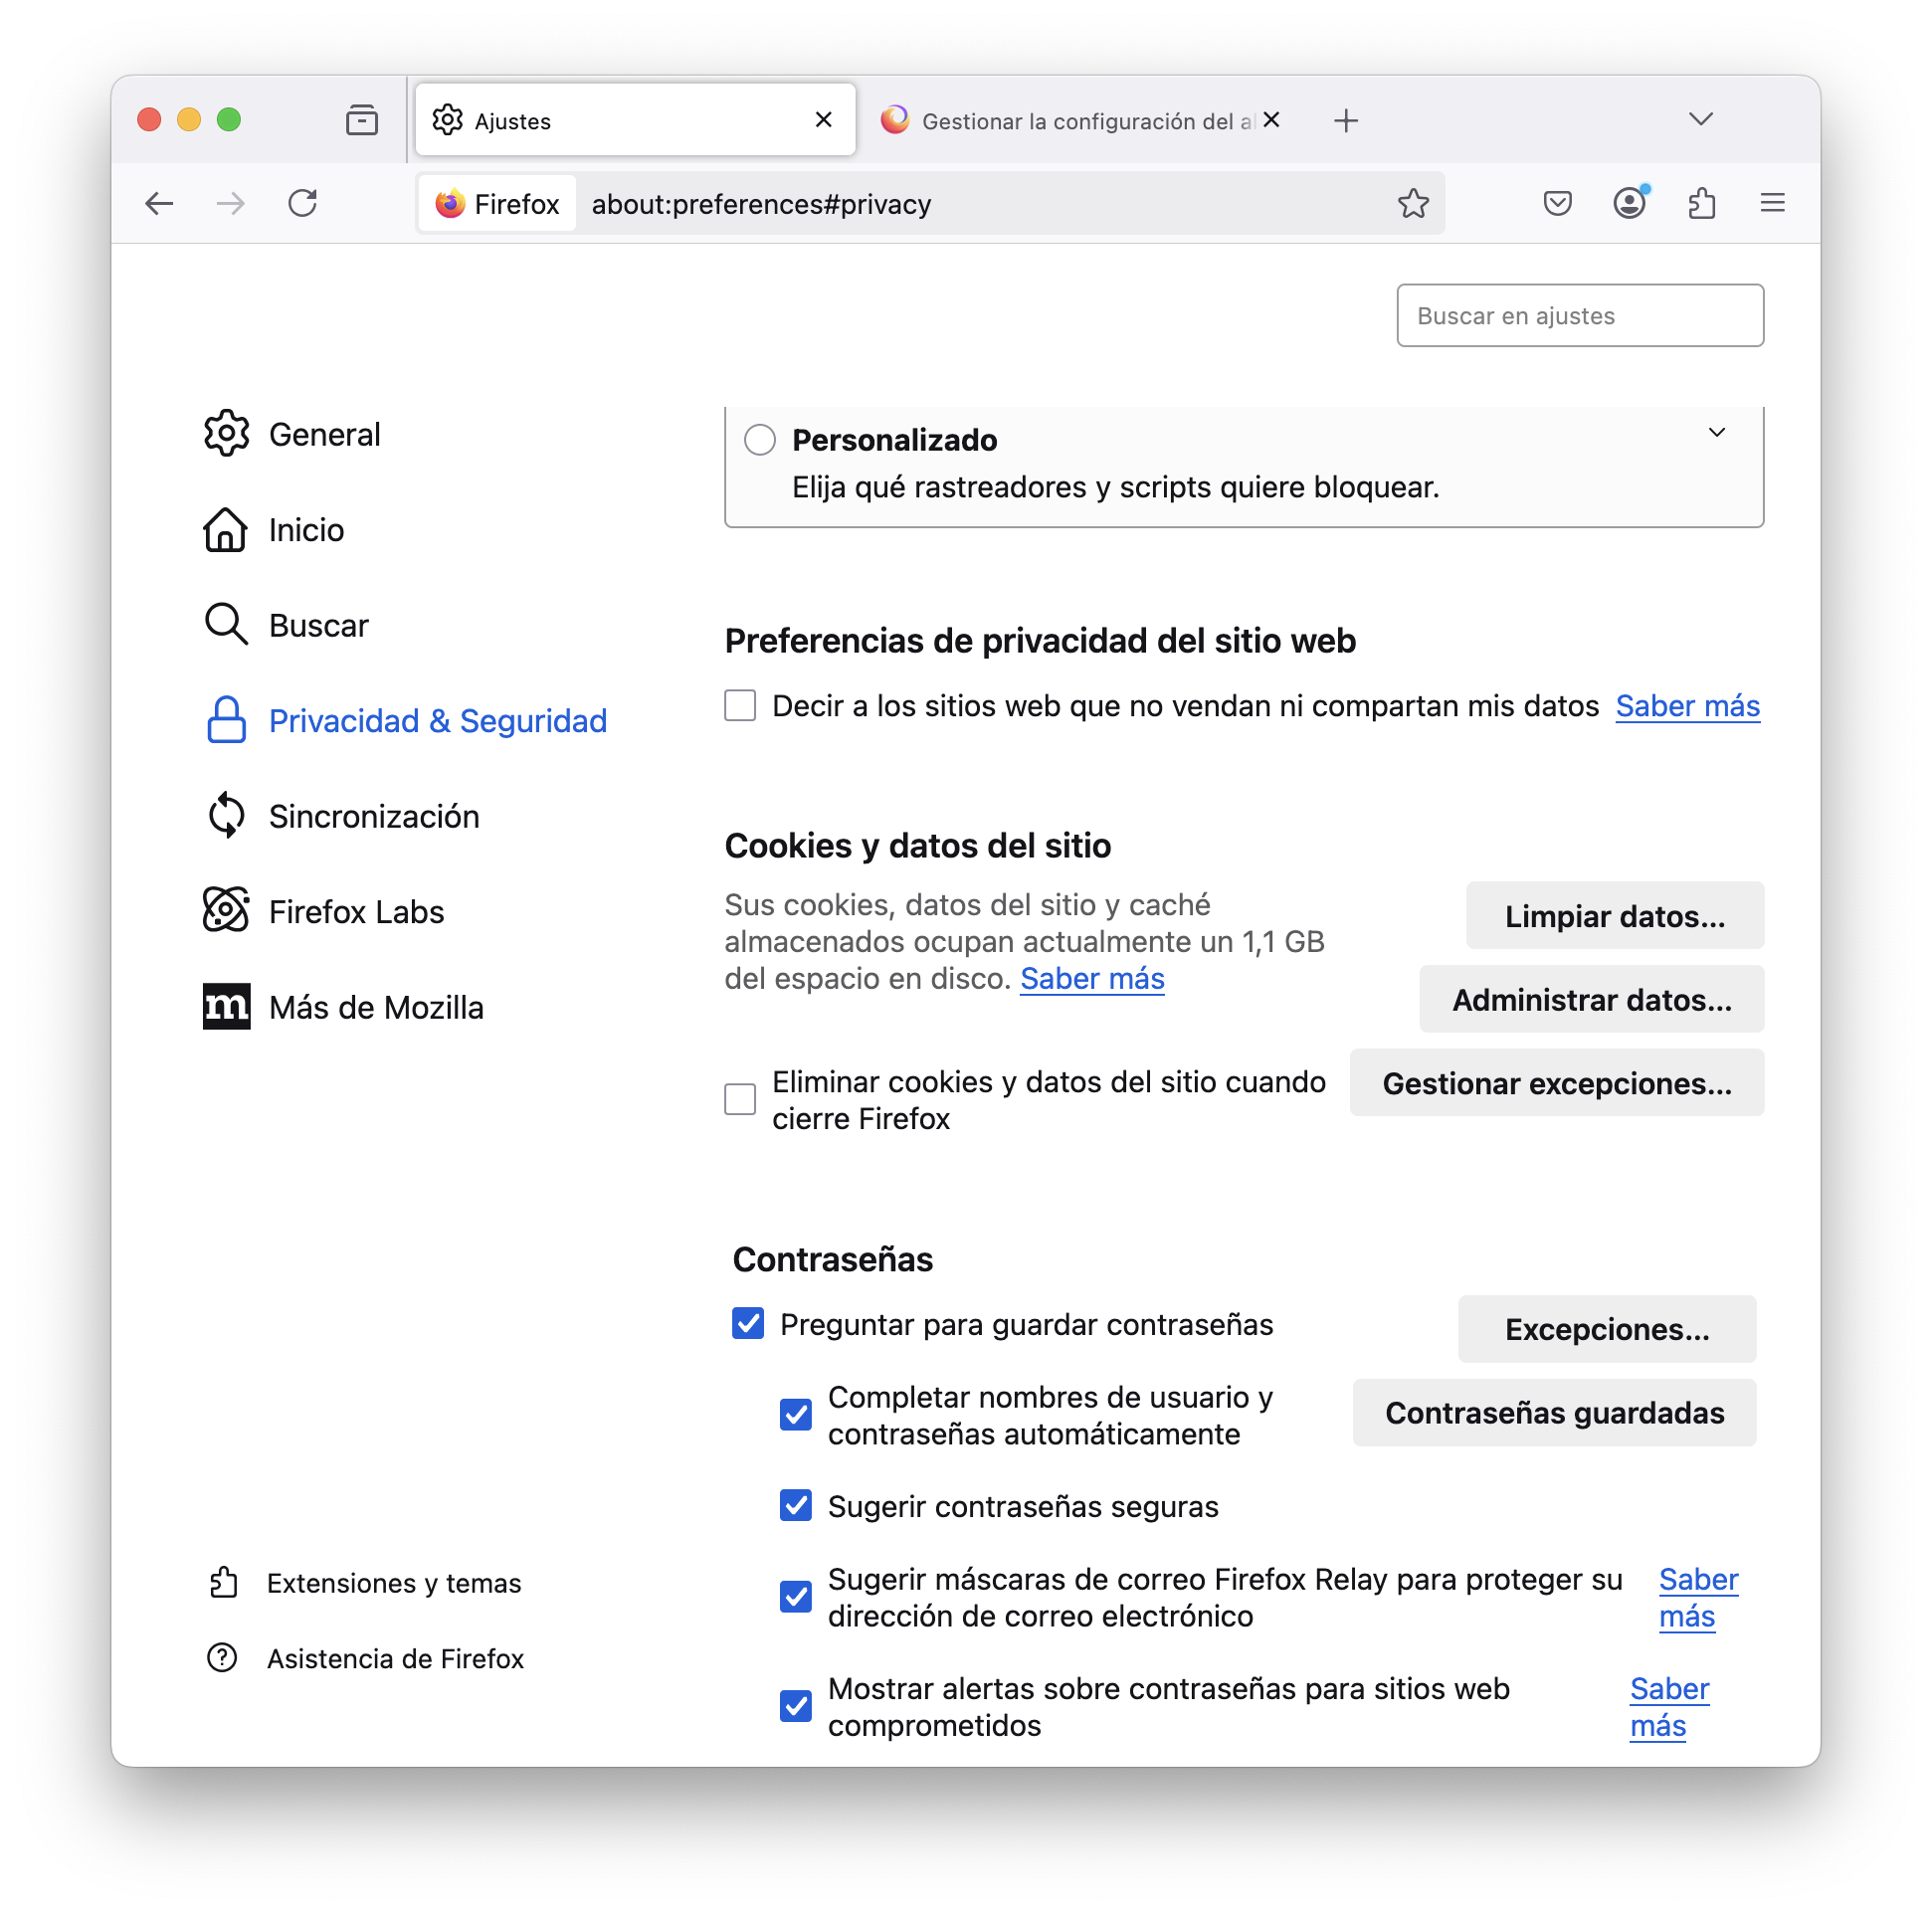
\includegraphics[width=15cm]{opcion1_ej14.png}
    \caption{Opción 1 de configuración de cookies, Firefox}
    \label{fig:opcion1_ej14}
\end{figure}


\paragraph{Eliminar almacenamiento del sitio en páginas individuales }

Esta opción borra los datos almacenados (como cookies) de una página web específica sin afectar a otras. Para poder aprovecharla, una vez estamos en la situación de que se muestra en la \ref{fig: opcion1_ej14} debemos seleccionar la opción "Administrar datos". Como se ve en la \ref{fig: opcion2_ej14}, aparecerá una lista de sitios y cuanta información almacena en el equipo del usuario. Ahí se podrá seleccionar el sitio que se desee para eliminar todas las cookies y datos almacenados. 

\begin{figure}[H]   
    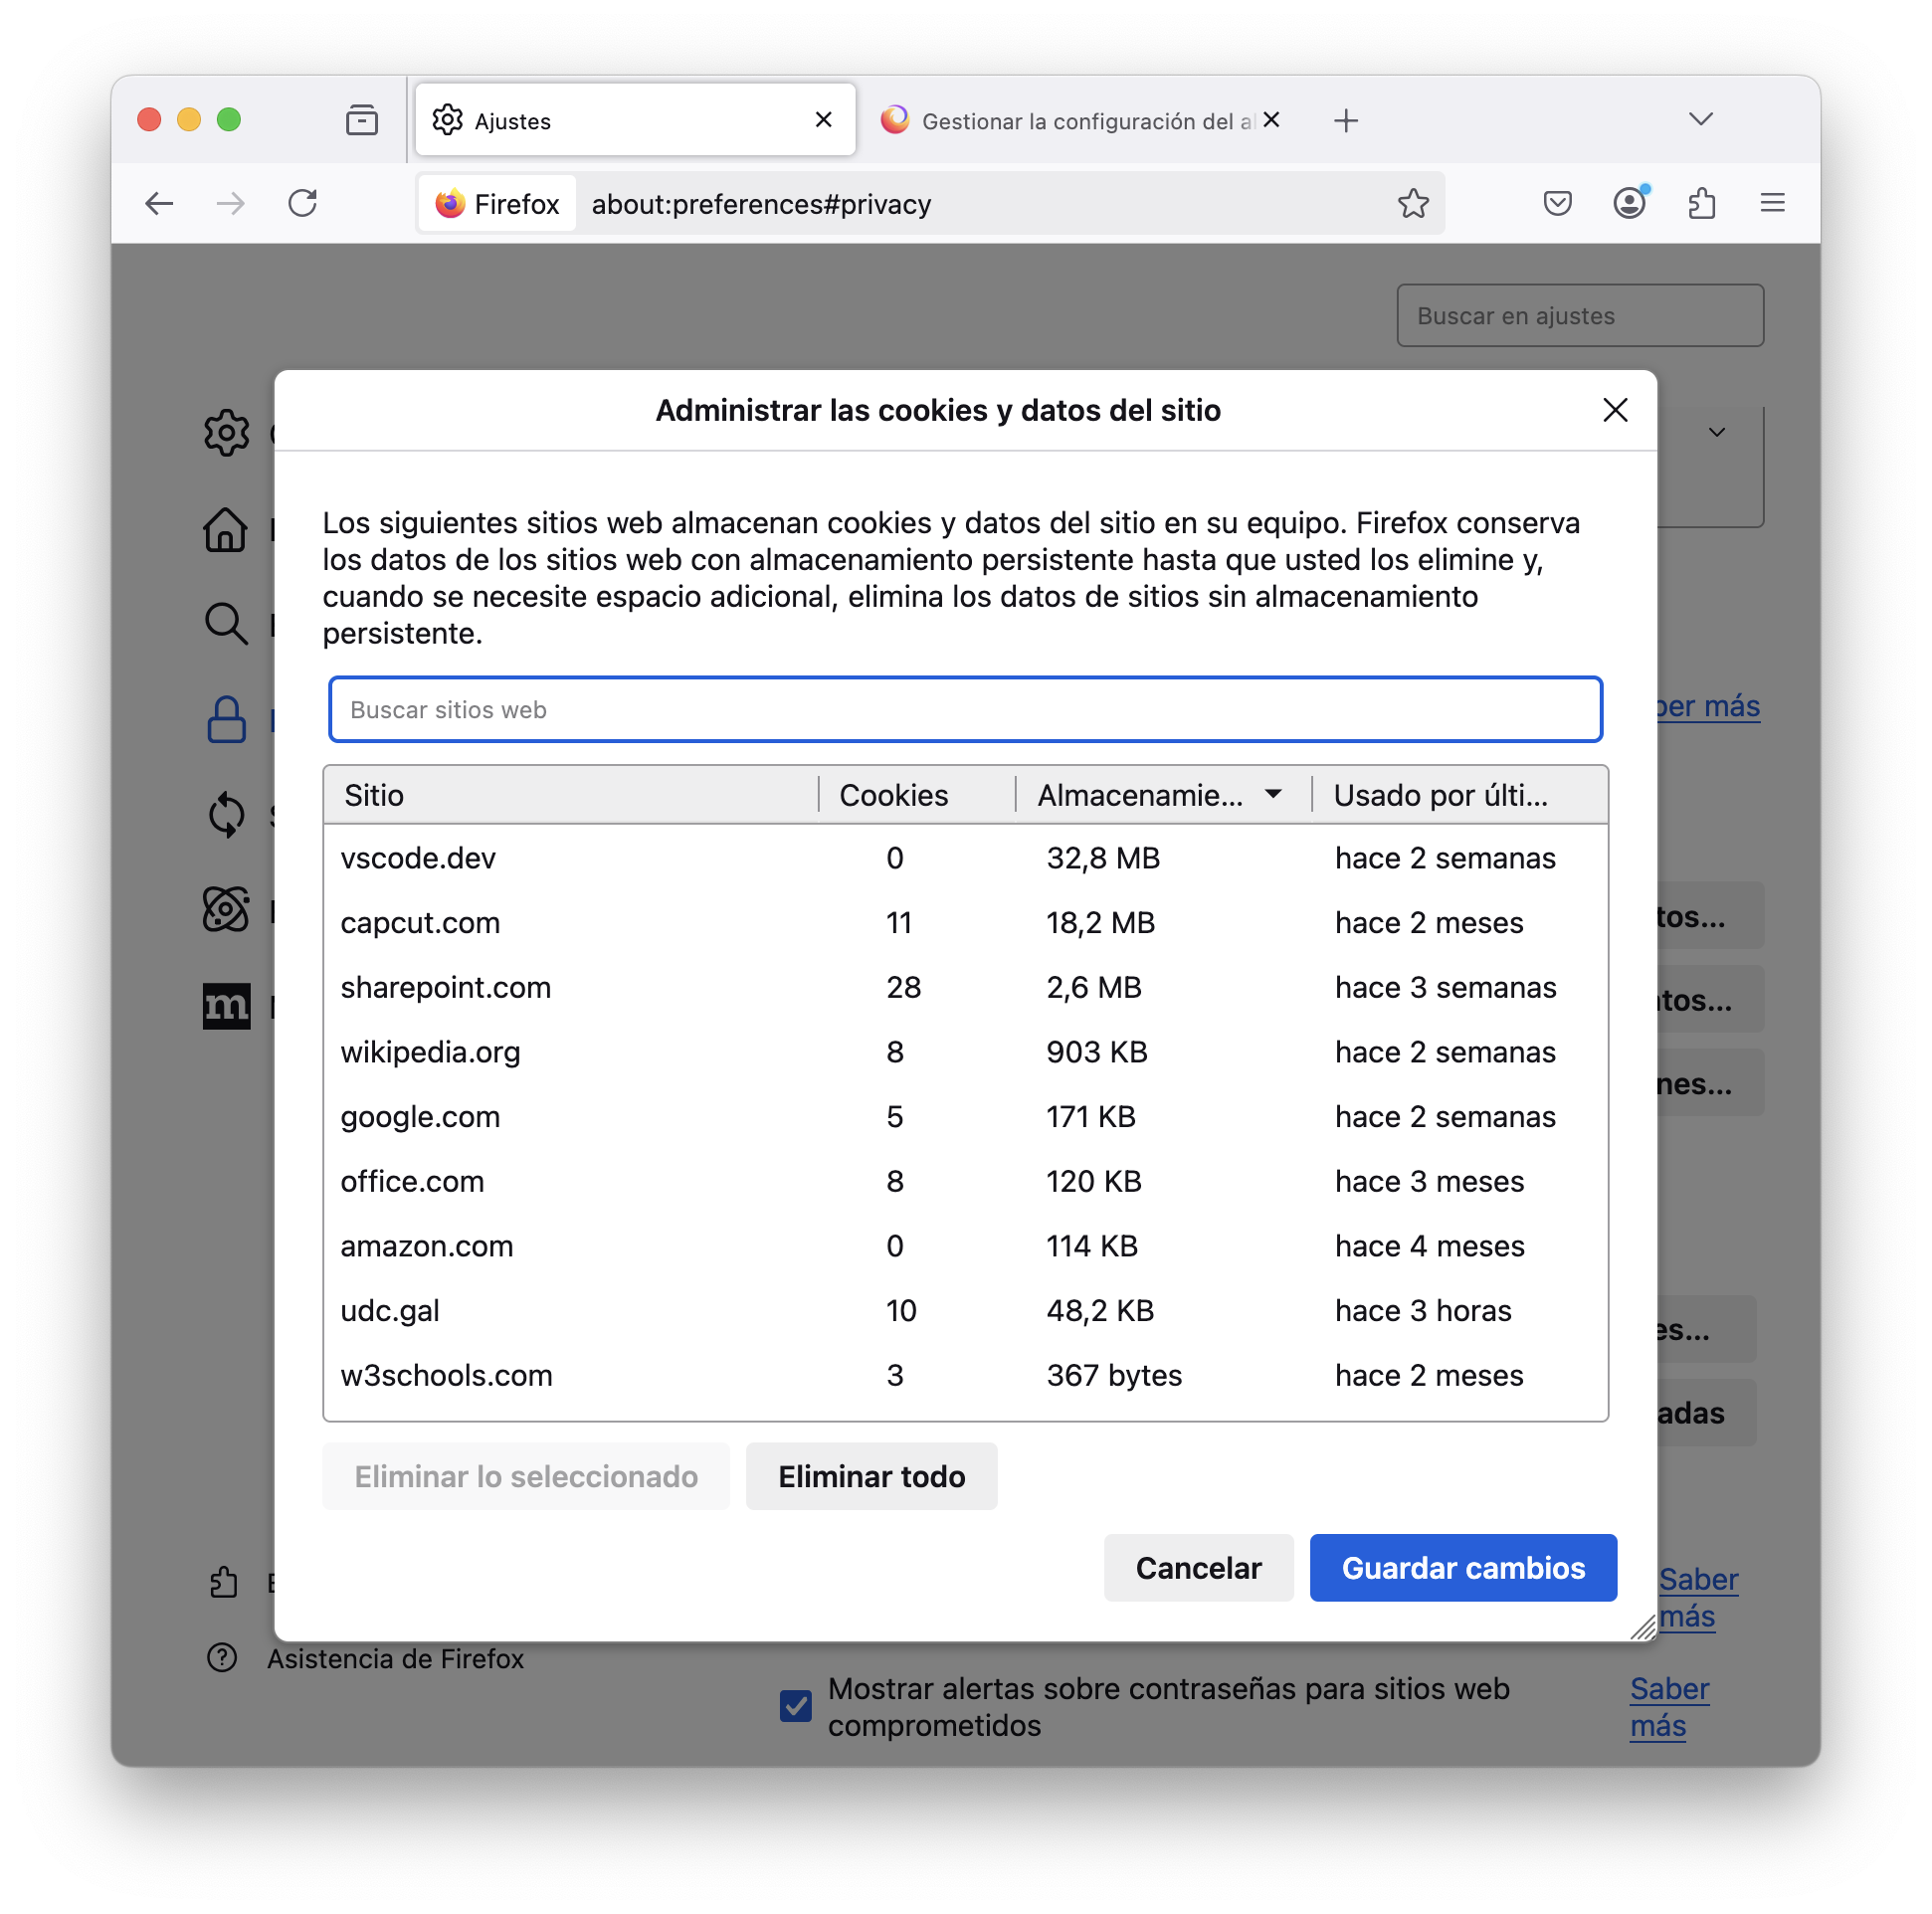
\includegraphics[width=15cm]{opcion2_ej14.png}
    \caption{Opción 2 de configuración de cookies, Firefox}
    \label{fig:opcion2_ej14}
\end{figure}

\paragraph{Eliminar los datos almacenados de todos los sitios}

Esta opción elimina todas las cookies y datos guardados de todos los sitios web visitados. Para poder aprovecharla, una vez estamos en la situación de que se muestra en la \ref{fig: opcion1_ej14}, debemos seleccionar la opción “Limpiar datos”. Como se ve en la \ref{fig: opcion3_ej14} se nos permite limpiar información de “cookies y datos del sitio” o “contenido de caché", entre otras. 

\begin{figure}[H]   
    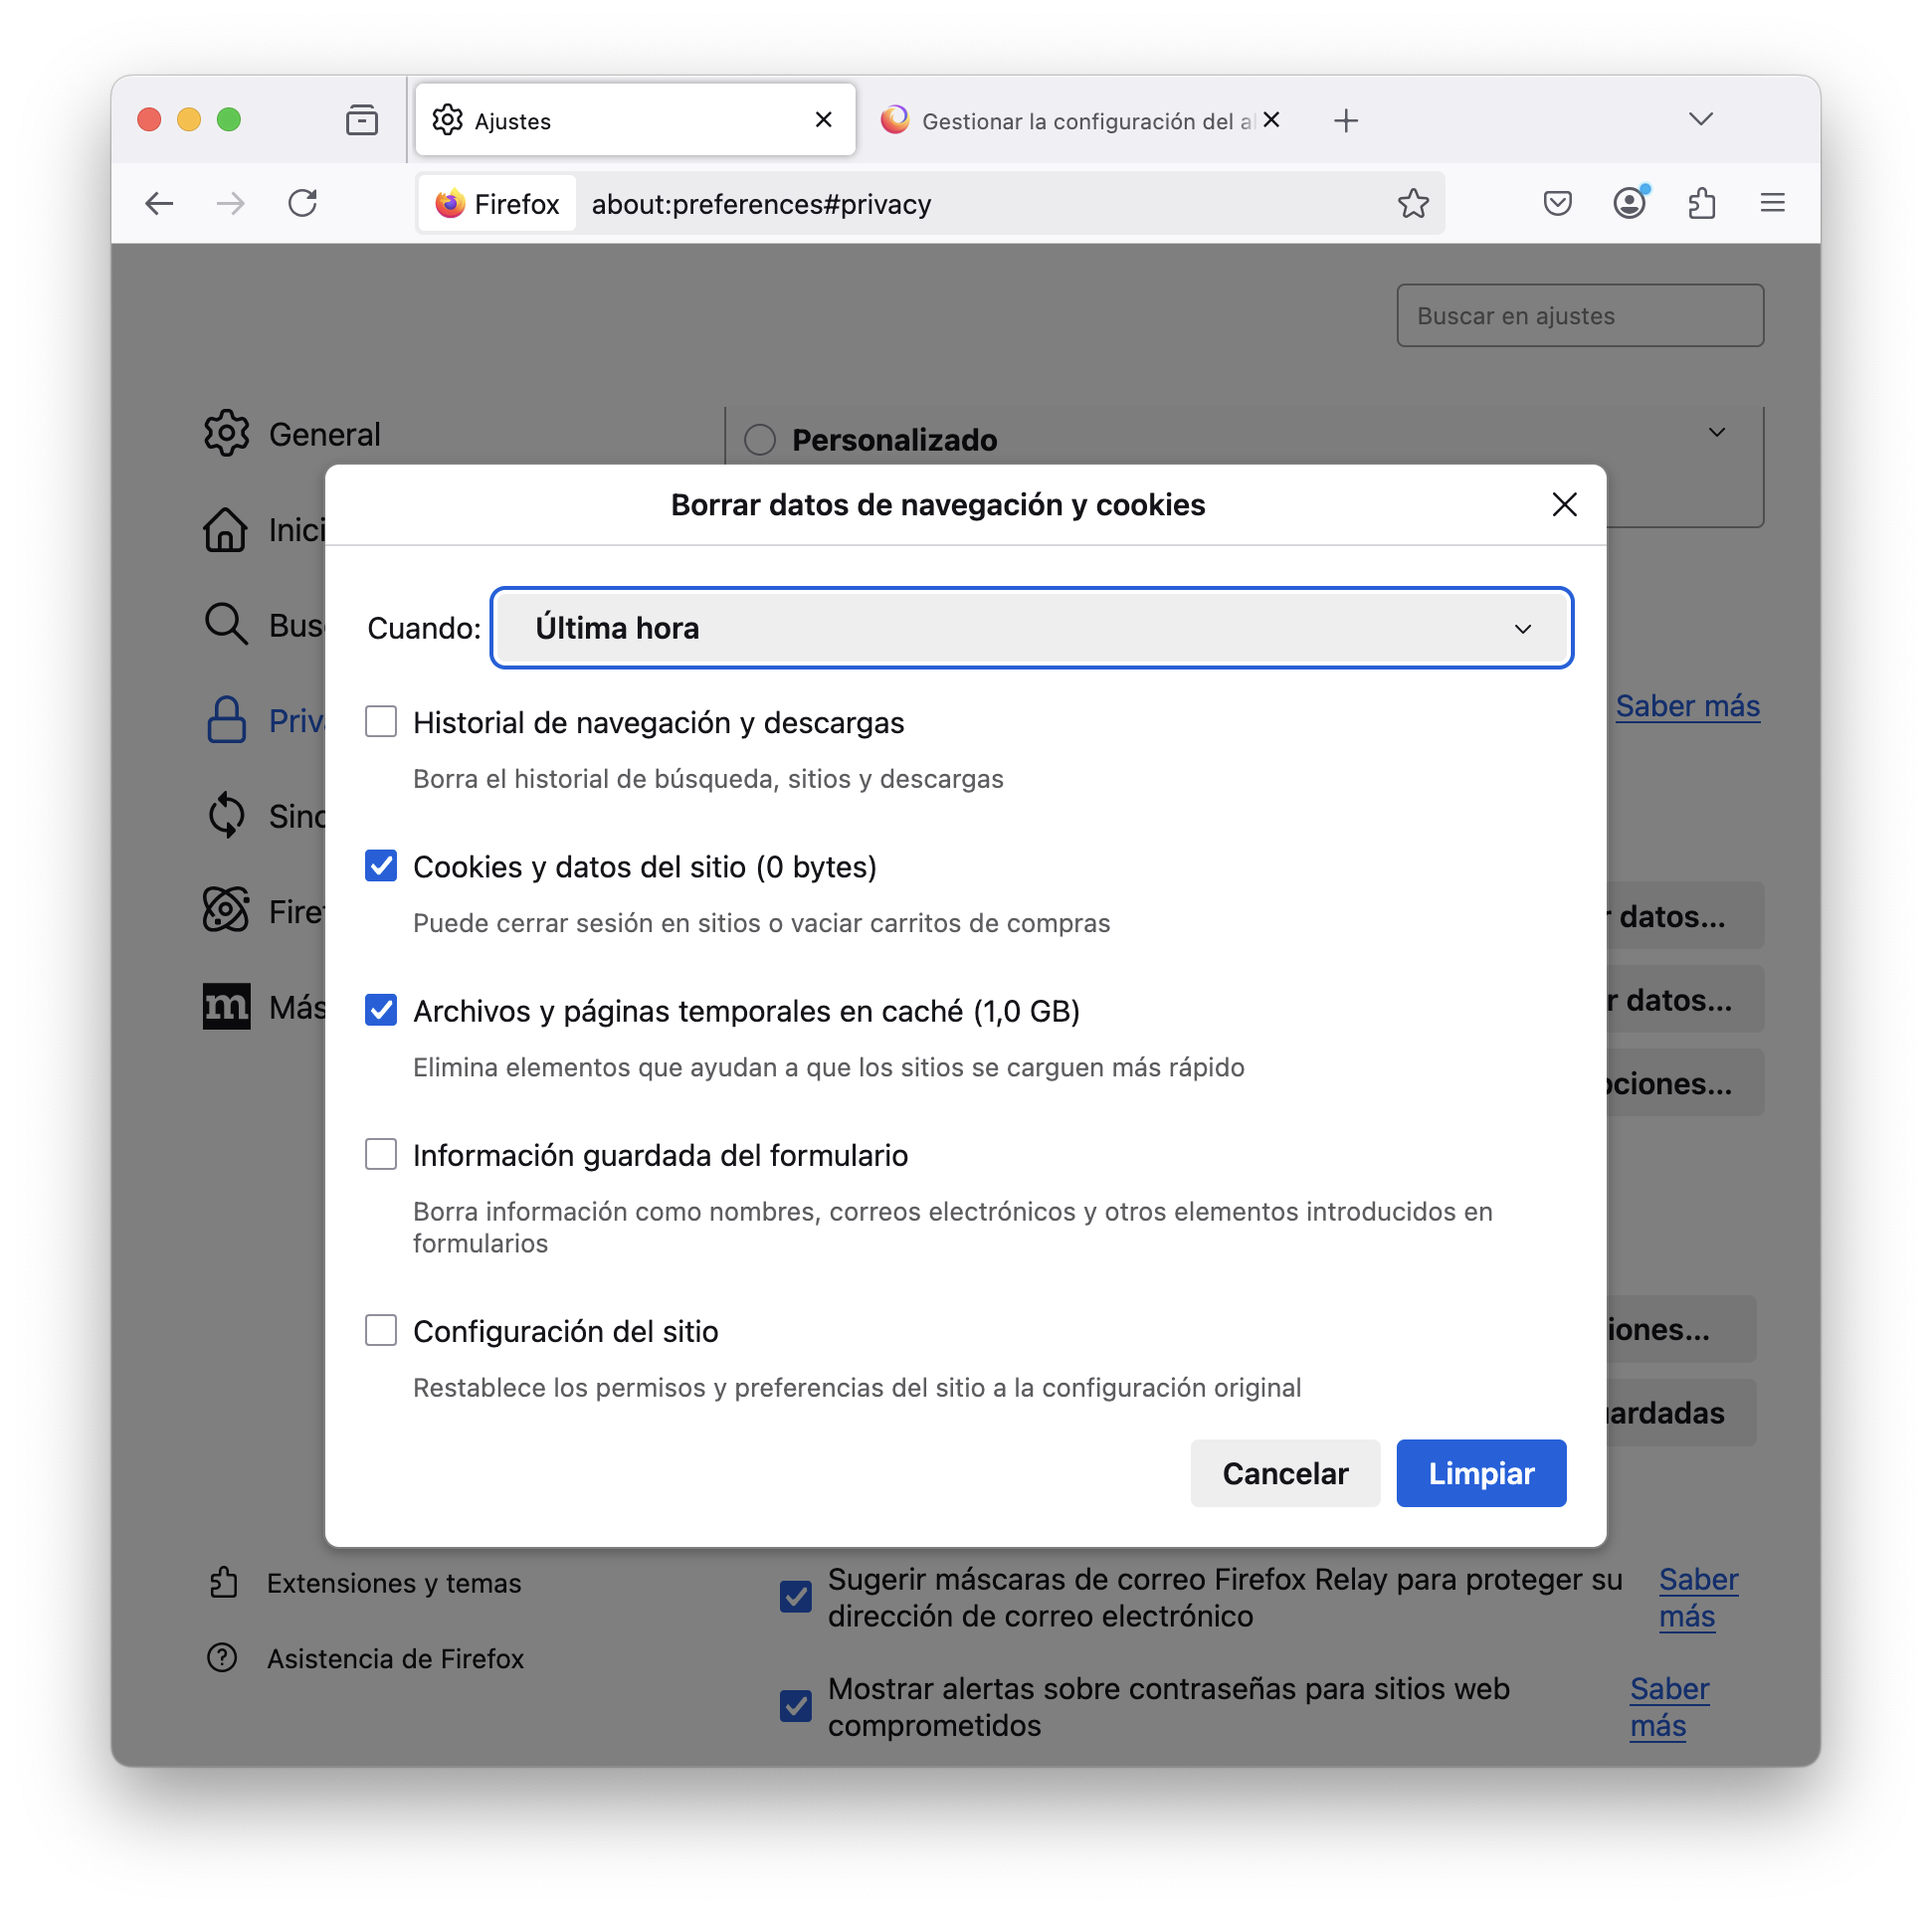
\includegraphics[width=15cm]{opcion3_ej14.png}
    \caption{Opción 3 de configuración de cookies, Firefox}
    \label{fig:opcion3_ej14}
\end{figure}

\paragraph{Permitir o bloquear a los sitios que almacenen información }

Esta opción da control al usuario para decidir qué sitios pueden guardar cookies y datos en su dispositivo. Para poder aprovecharla, una vez estamos en la situación de que se muestra en la \ref{fig: opcion3_ej14}, debemos seleccionar la opción “Gestionar excepciones”. Como se ve en la \ref{fig: opcion4_ej14}, se nos permite escribir la dirección exacta del sitio a permitir o bloquear. 

\begin{figure}[H]   
    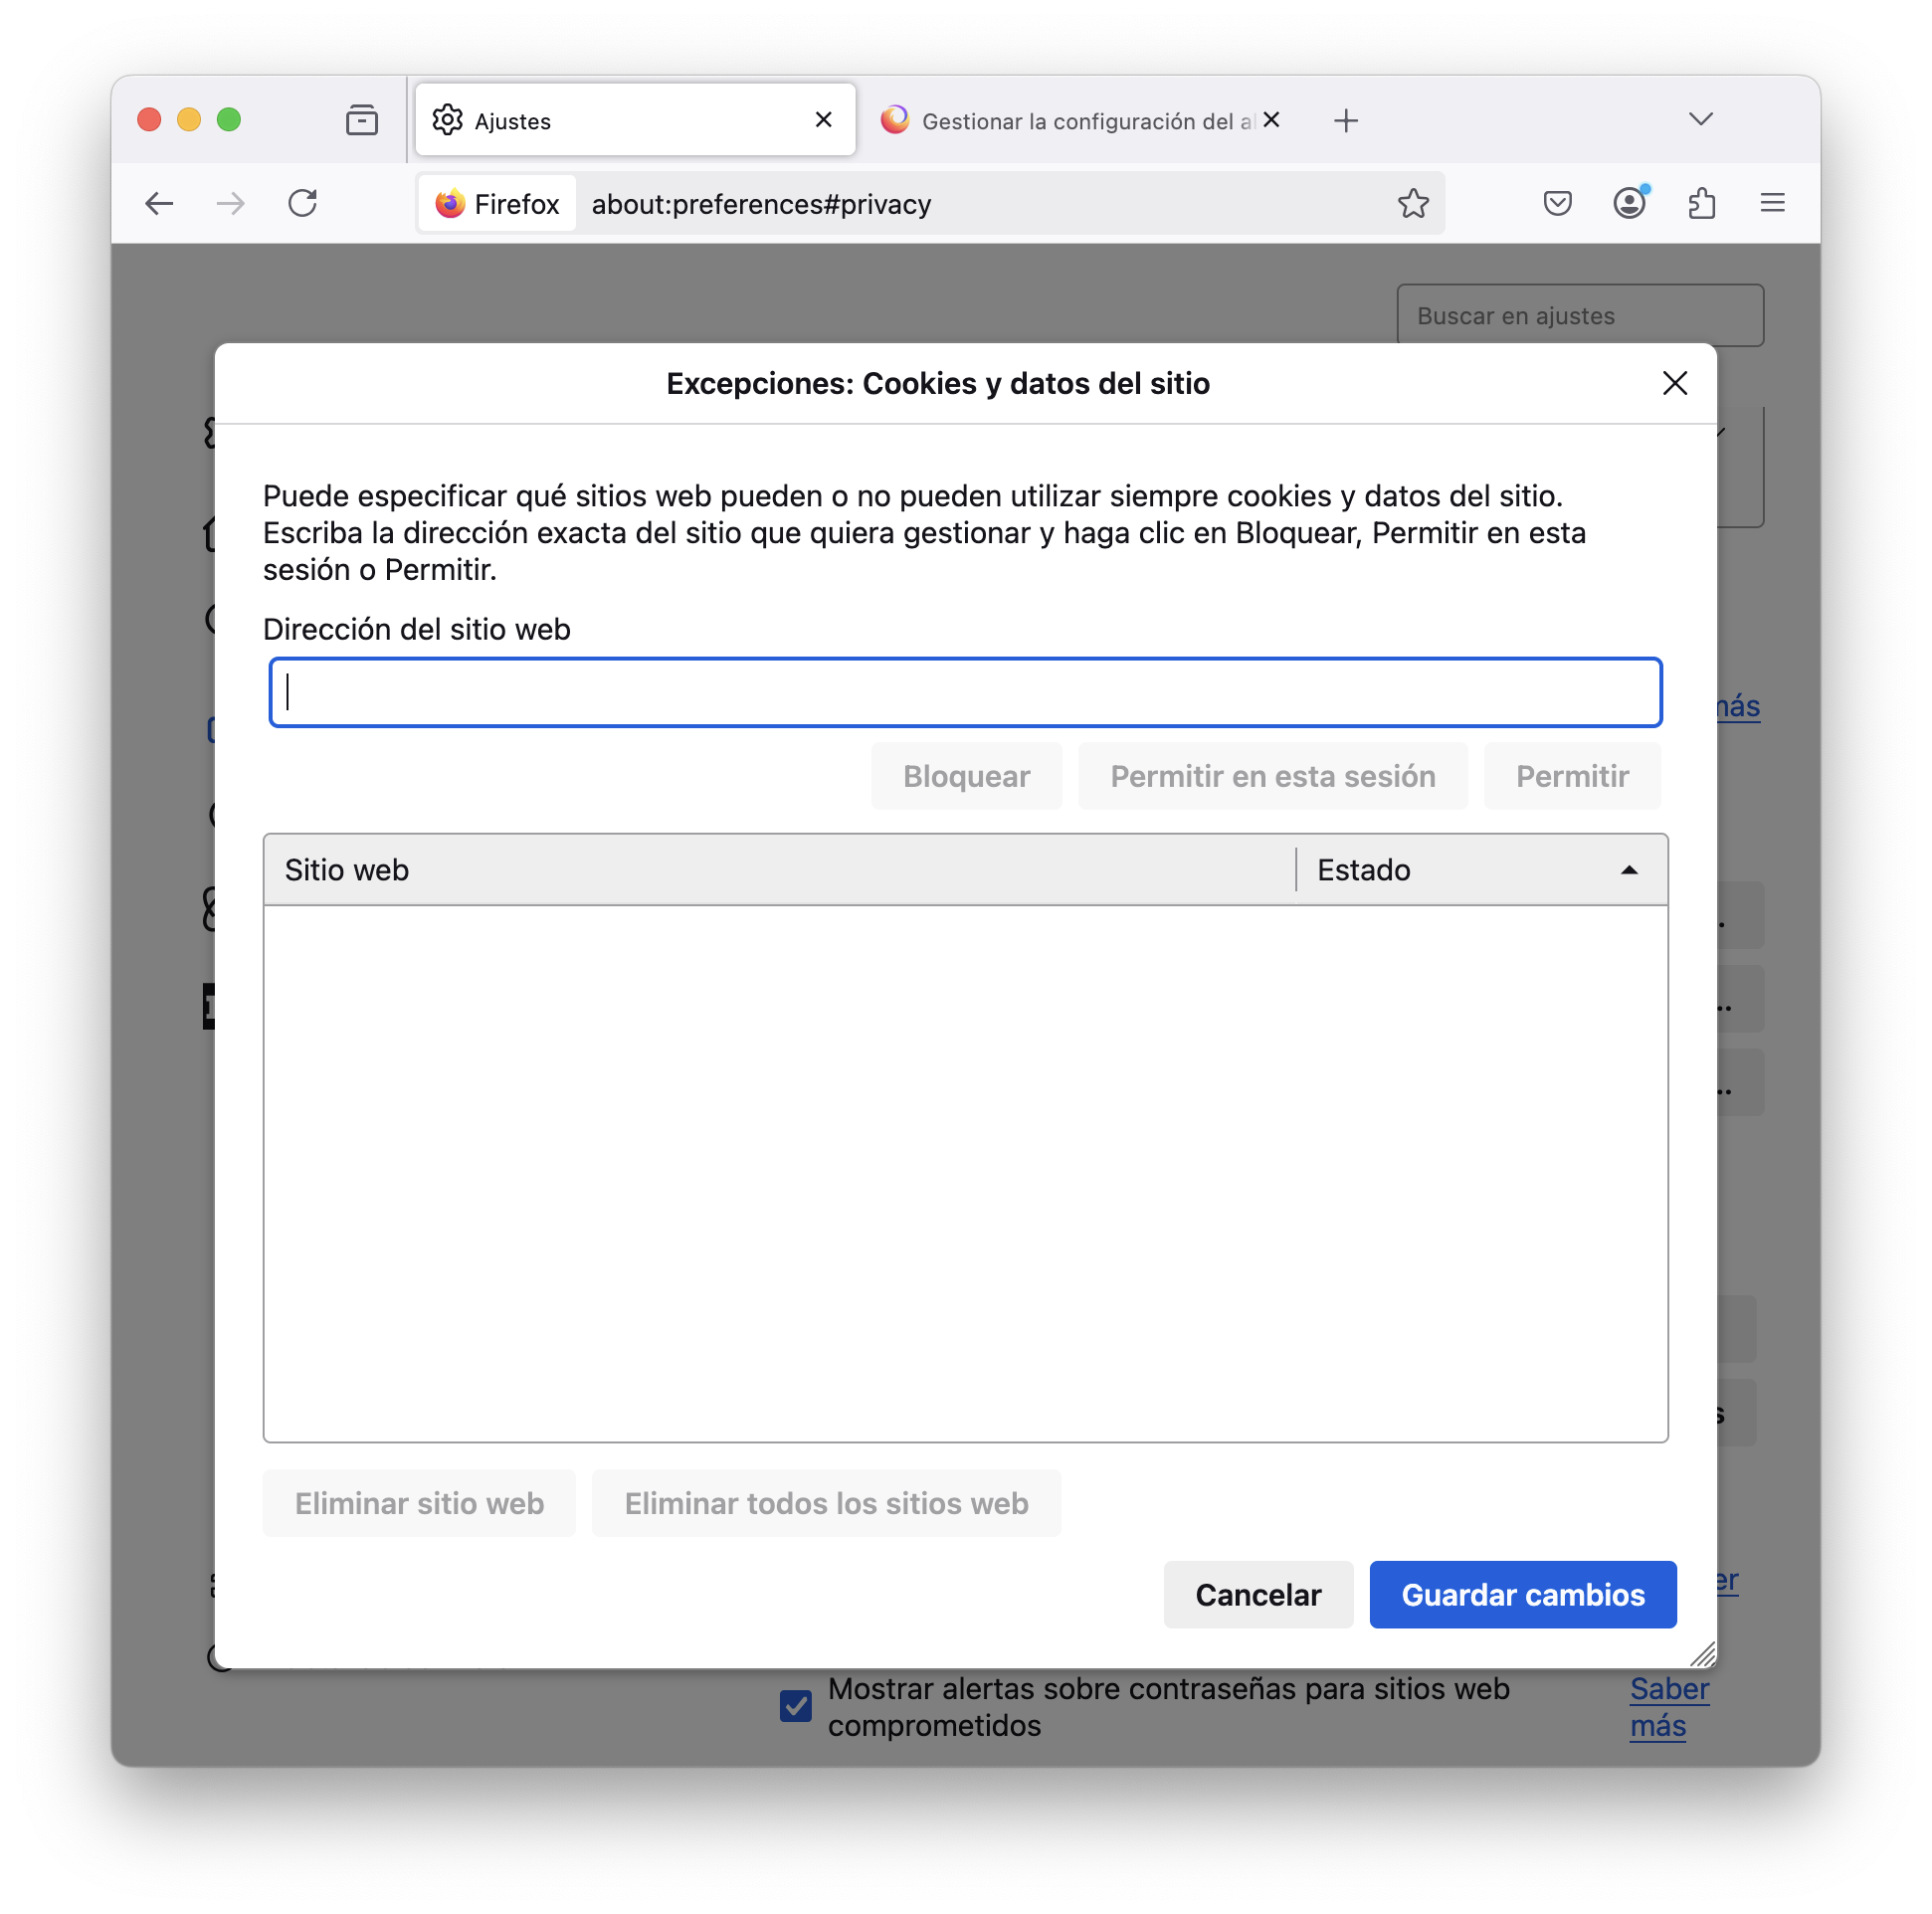
\includegraphics[width=15cm]{opcion4_ej14.png}
    \caption{Opción 4 de configuración de cookies, Firefox}
    \label{fig:opcion4_ej14}
\end{figure}


\subsubsection{Configuración cookies Chrome y LibreWolf}

Para poder ver las opciones de gestión de cookies en Google Chrome debemos acceder al menú de configuración y una vez ahí, como se ve en la \ref{fig: cookies_chrome}, podemos acceder a la configuración de "Cookies de terceros". Ahí nos encontramos con tres opciones: 

\paragraph{Permitir cookies de terceros}

Esta opción permite que todos los sitios web usen cookies para seguimiento, personalización o publicidad. 

\paragraph{Bloquear cookies de terceros en modo Incógnito}

Esta opción impide que terceros usen cookies solo cuando se navega en modo incógnito, limitando el rastreo sin afectar la navegación normal. 

\paragraph{Bloquear cookies de terceros}

Esta opción evita completamente que sitios externos a los que se visita usen cookies, aumentando la privacidad pero pudiendo afectar funciones de algunas webs. 

\paragraph{Enviar una solicitud "Do Not Track" con tu tráfico de navegación }

Esta opción solicita a los sitios que no rastreen la actividad del usuario, aunque pueden ignorarlo porque es voluntario. 

\begin{figure}[H]   
    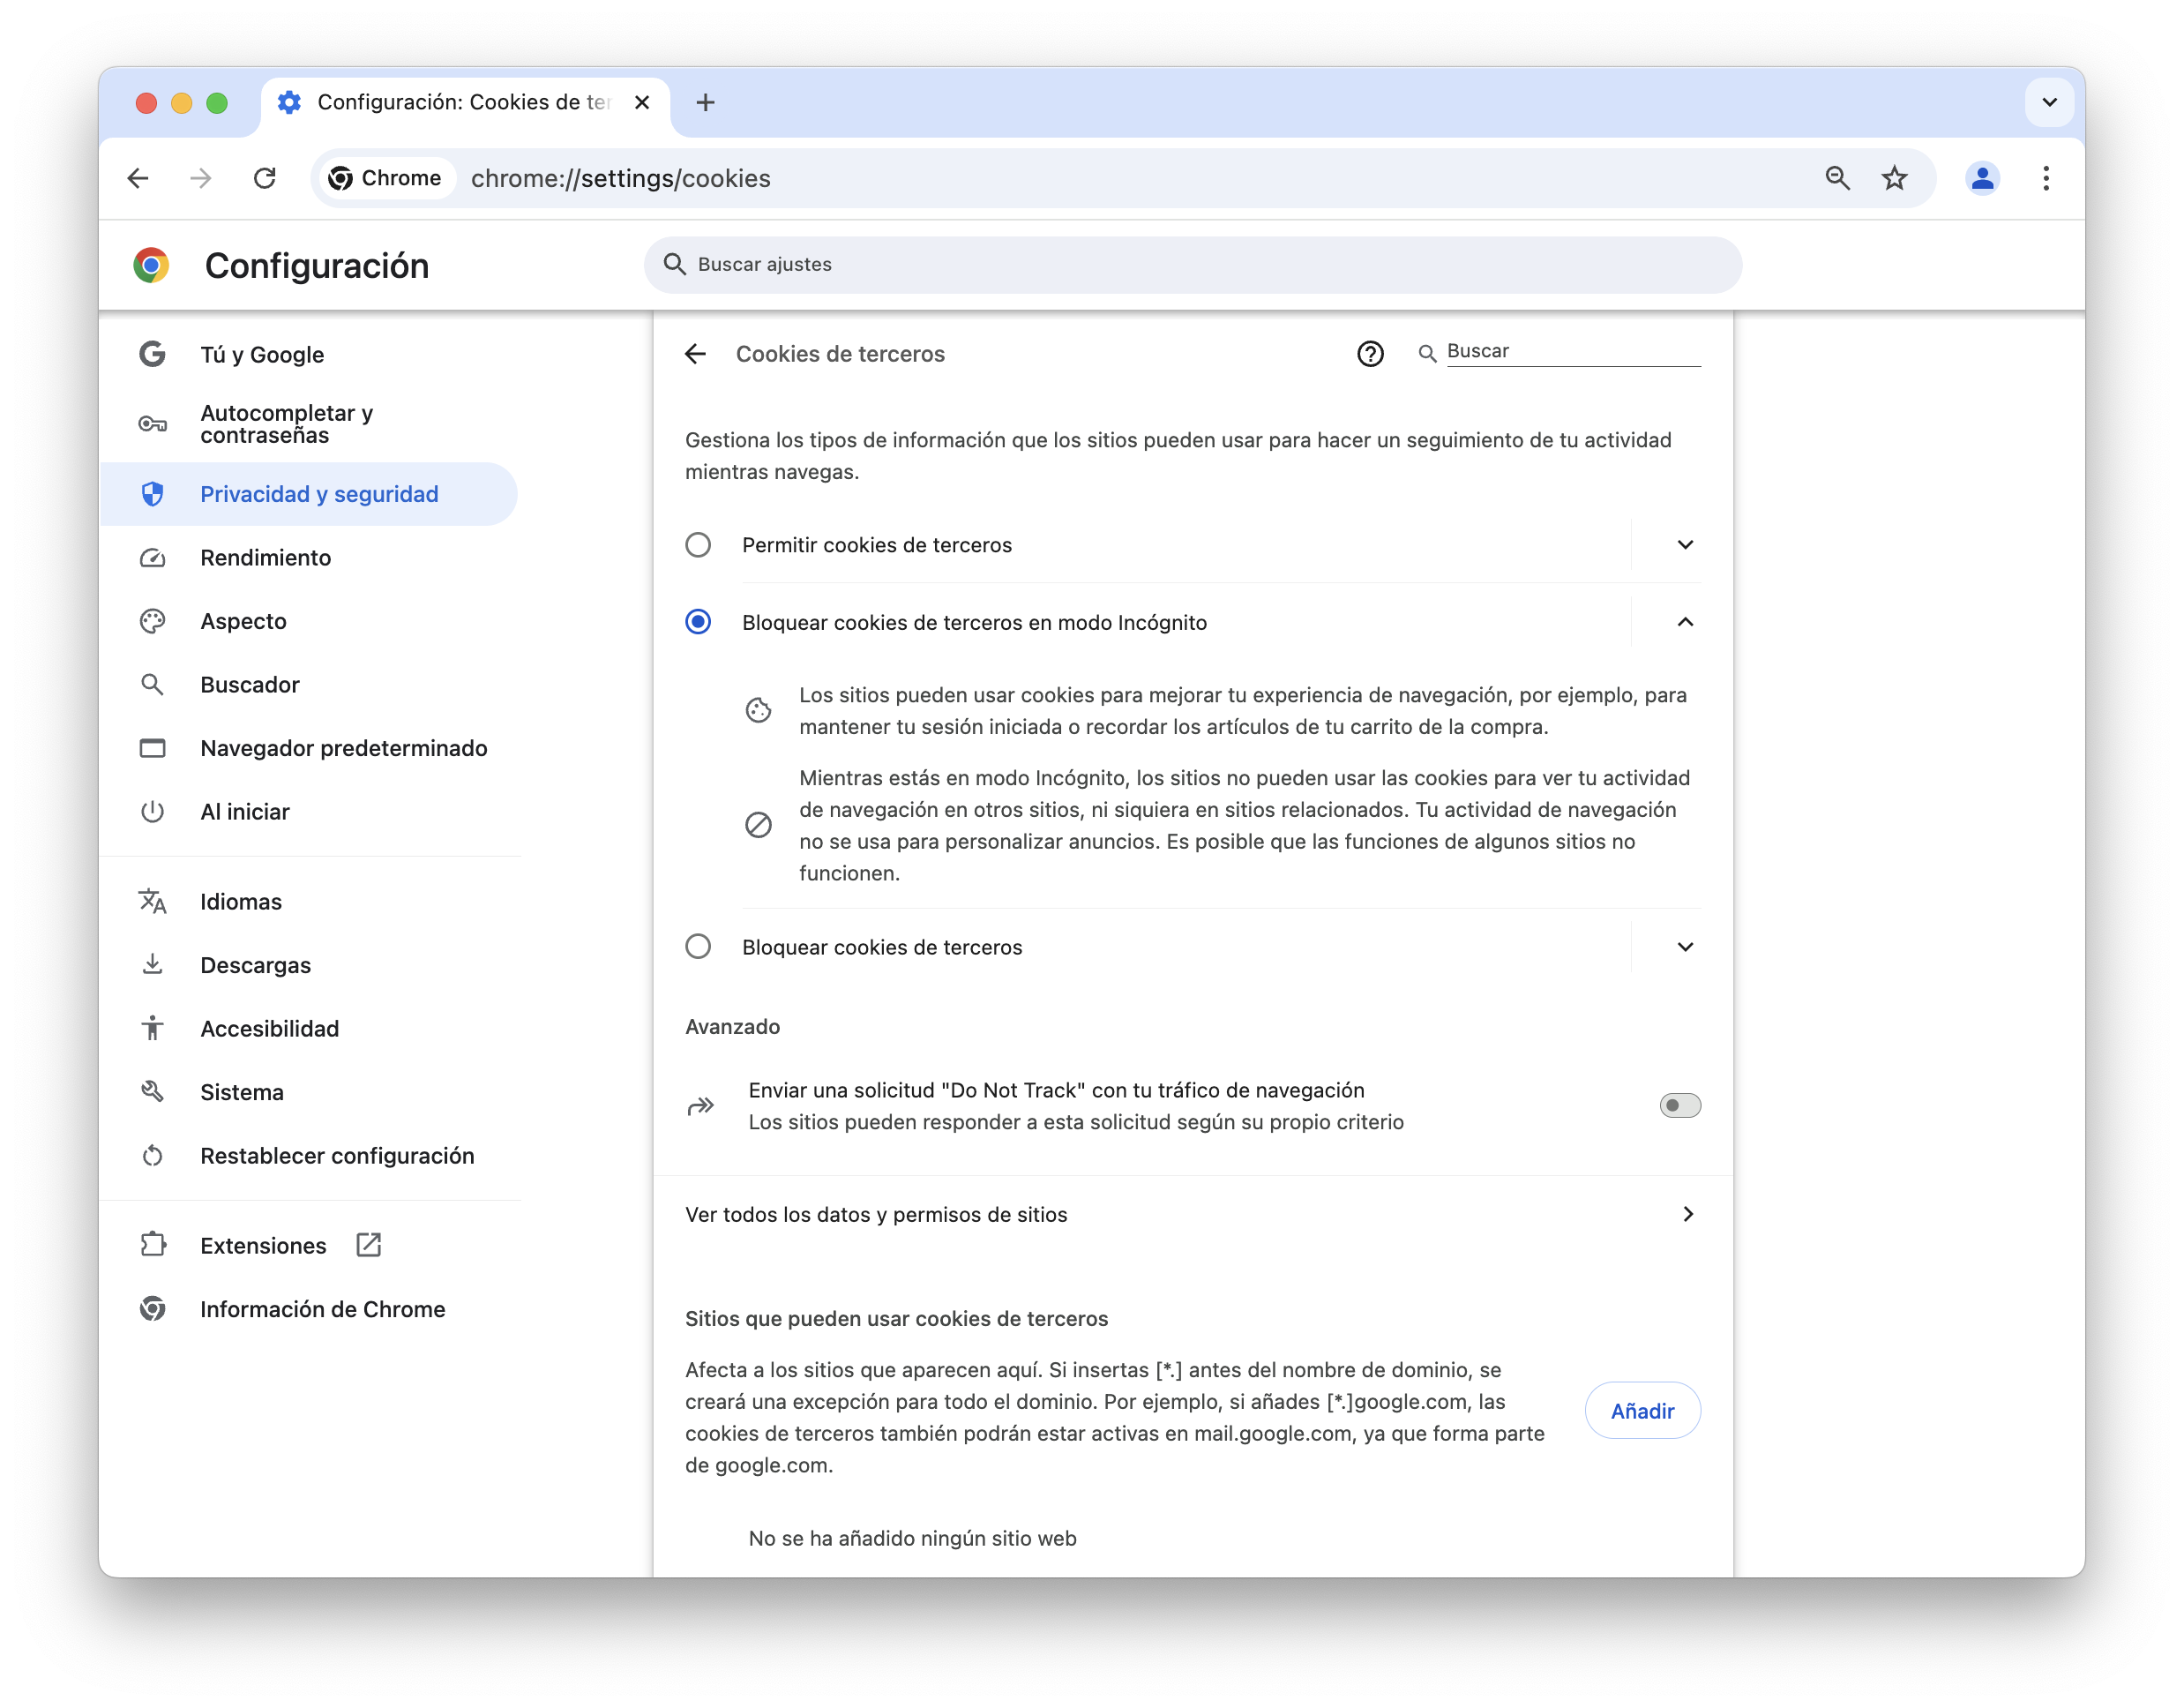
\includegraphics[width=15cm]{cookies_chrome_ej14a.png}
    \caption{Configuración de cookies en Chrome}
    \label{fig:cookies_chrome}
\end{figure}

Por otro lado, para acceder a la configuración de cookies de Librewolf, seguimos los pasos anteriores hasta llevar a la \ref{fig: cookies_librewolf}. Como se aprecia, las opciones son aparentemente las mismas que en Mozilla Firefox, explicadas en el apartado anterior. Esto se debe a que Firefox y LibreWolf son navegadores basados en el mismo motor, pero con enfoques diferentes en cuanto a privacidad y control del usuario. Mientras que Firefox ofrece un equilibrio entre personalización, compatibilidad y privacidad, LibreWolf está diseñado específicamente para proteger al máximo la privacidad desde el primer uso. LibreWolf desactiva por defecto toda la telemetría, bloquea rastreadores y cookies de terceros, elimina automáticamente los datos al cerrar el navegador y no incluye integración con servicios de Mozilla. En cambio, Firefox requiere que el usuario configure manualmente muchas de estas opciones para alcanzar el mismo nivel de privacidad. 

\begin{figure}[H]   
    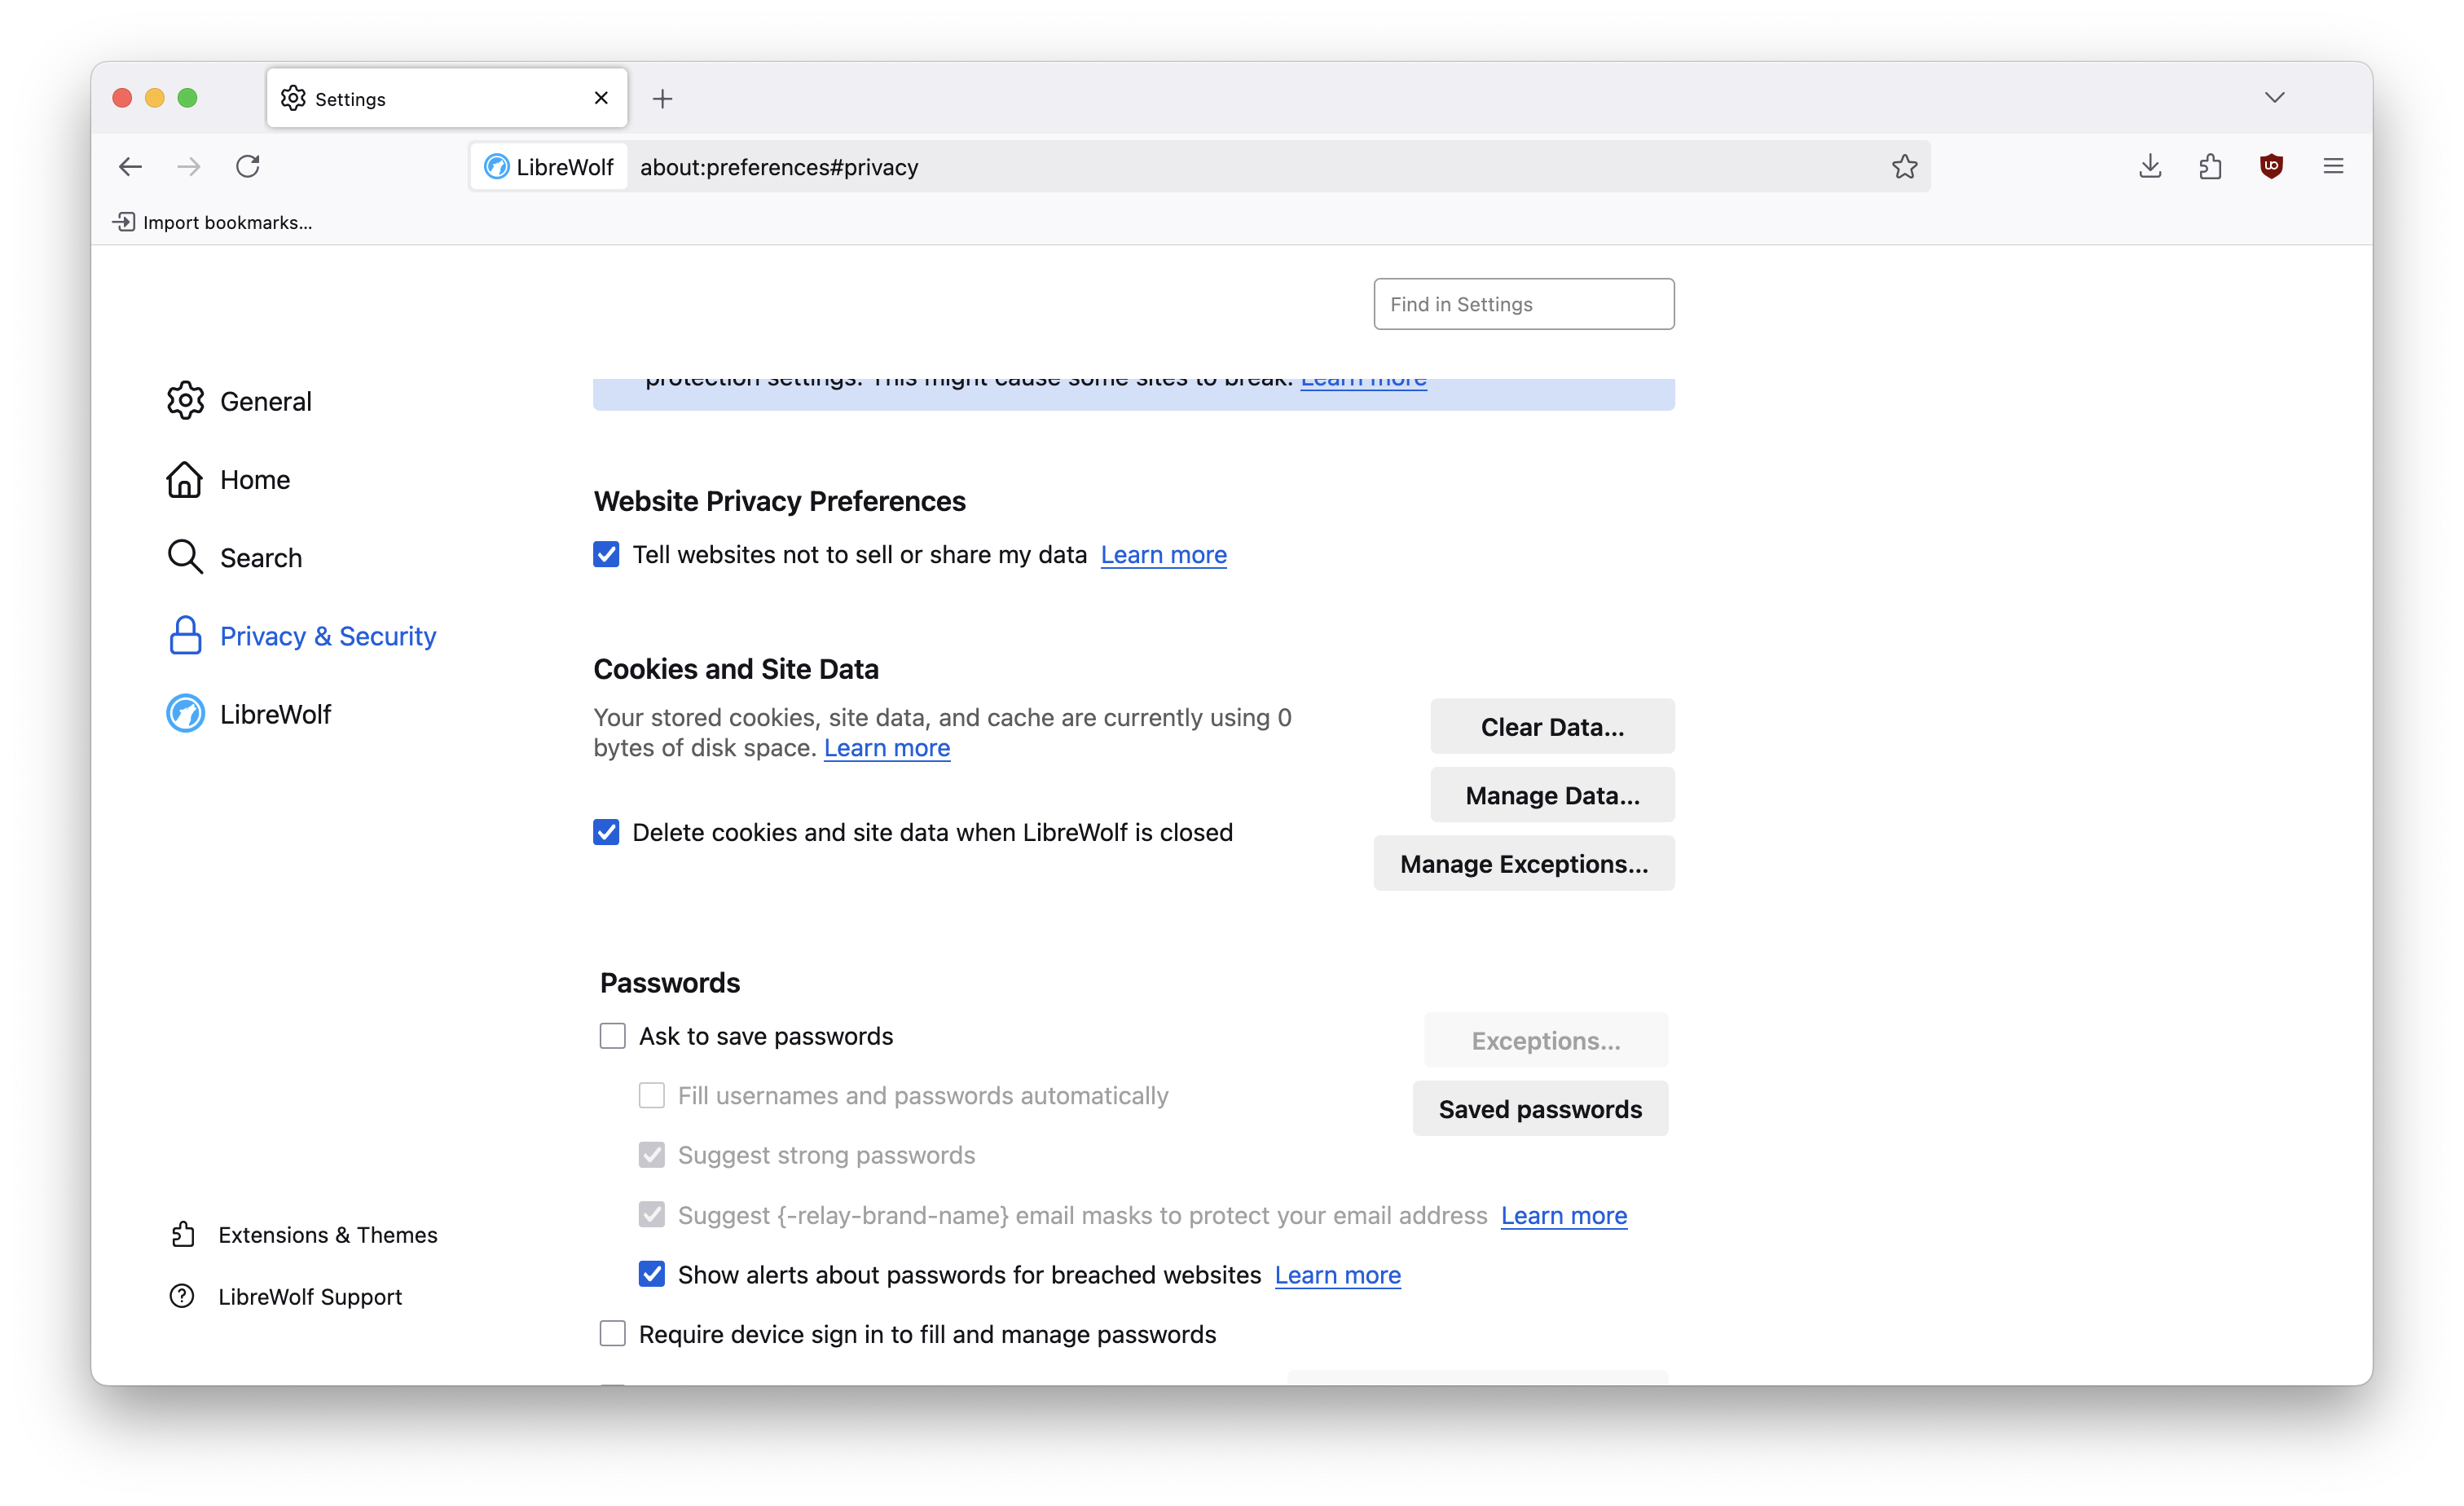
\includegraphics[width=15cm]{cookies_librewolf_ej14a.png}
    \caption{Configuración de cookies en LibreWolf}
    \label{fig:cookies_librewolf}
\end{figure}

En \ref{comparativa-cookies} podemos ver una comparación más visual de los 3 buscadores.

\begin{table}[H]
    \centering
    \begin{tabular}{|l|c|c|c|}
    \hline
    \textbf{Característica} & \textbf{Firefox} & \textbf{LibreWolf} & \textbf{Chrome} \\ \hline
    Permitir todas las cookies & Sí (manual) & No (privacidad estricta) & Sí (por defecto) \\ \hline
    Bloquear cookies de terceros & Sí (opción manual) & Sí (activado por defecto) & Sí (opción disponible) \\ \hline
    Eliminar cookies al cerrar & Opcional & Activado por defecto & Opcional \\ \hline
    Telemetría y rastreo & Activado (puede desactivarse) & Desactivado & Activado (puede limitarse) \\ \hline
    Protección de privacidad & Alta (manual) & Muy alta (por defecto) & Media (requiere configurarlo) \\ \hline
    \end{tabular}
    \caption{Comparativa de opciones de configuración de cookies en Firefox, LibreWolf y Chrome.}
    \label{tab:comparativa-cookies}
\end{table}

\subsubsection{Extensiones de navegador para la gestión de cookies}

\paragraph{Cookie AutoDelete}

Cookie AutoDelete es una extensión de navegador diseñada para gestionar automáticamente las cookies y otros datos de sitios web. Su principal función es eliminar las cookies asociadas a una pestaña en cuanto esta se cierra, evitando que los sitios web rastreen al usuario en futuras visitas. Además, permite crear listas blancas (whitelists) para conservar las cookies de sitios de confianza y listas grises (greylists) para eliminar cookies al reiniciar el navegador. La extensión también ofrece opciones para eliminar manualmente cookies y otros datos de almacenamiento, como IndexedDB y LocalStorage, y es compatible con las pestañas de contenedor en Firefox [\url{cookie_autodelete.gal}]

\paragraph{Privacy Badger}

Privacy Badger, desarrollado por la Electronic Frontier Foundation (EFF), es una extensión de navegador que bloquea automáticamente rastreadores invisibles y cookies de terceros sin necesidad de configuración previa. A diferencia de los bloqueadores tradicionales basados en listas predefinidas, Privacy Badger utiliza un algoritmo de aprendizaje automático que detecta y bloquea dominios en función de su comportamiento de rastreo a lo largo de los sitios web visitados. Además, Privacy Badger envía señales como "Do Not Track" y "Global Privacy Control" para solicitar a los sitios web que no rastreen ni vendan la información del usuario. Si un dominio ignora estas señales y sigue rastreando, Privacy Badger lo bloquea automáticamente, fortaleciendo la privacidad de la navegación sin necesidad de intervención manual [\url{privacybadger.gal}]. 

\paragraph{Pruebas}

Para probar ambas extensiones del navegador, debemos instalarlas. En nuestro caso, elegimos Firefox como navegador. En las \ref{fig: addon_cookie_autodelete} y \ref{fig:addon_privacybadger} se ven las extensiones a instalar. Tras la instalación, se debe activar la extensión en el navegador de Cookie Autodelete, como se ve en la \ref{fig: activacion_cookie_autodelete}, mientras que Privacy Badger aparece automáticamente en la barra de extensiones. 

El siguiente paso es buscar una página web que utilice cookies. Lo ideal es hacer la prueba con páginas grandes que suelan tener rastreadores, como medios de comunicación o redes sociales. En nuestro caso, elegimos la página web del periódico La Voz de Galicia.  

Como se ve en \ref{fig:cookies_lavoz}, al entrar en la página nos aparece una pestaña para gestionar las cookies. Para comprobar el funcionamiento de las extensiones, debemos aceptar las cookies del sitio. Inmediatamente, aparecerán notificaciones de ambas extensiones, indicando que se han detectado correctamente los rastreadores y cookies. En \ref{fig:resultado_cookies_autodelete} y \ref{fig:resultado_privacybadger} vemos los resultados. Destacamos que Privacy Badger señala de color verde a los rastreadores que permite, de amarillo a los rastreadores que permite parcialmente, y de rojo a los bloqueados. 

\begin{figure}[H]   
    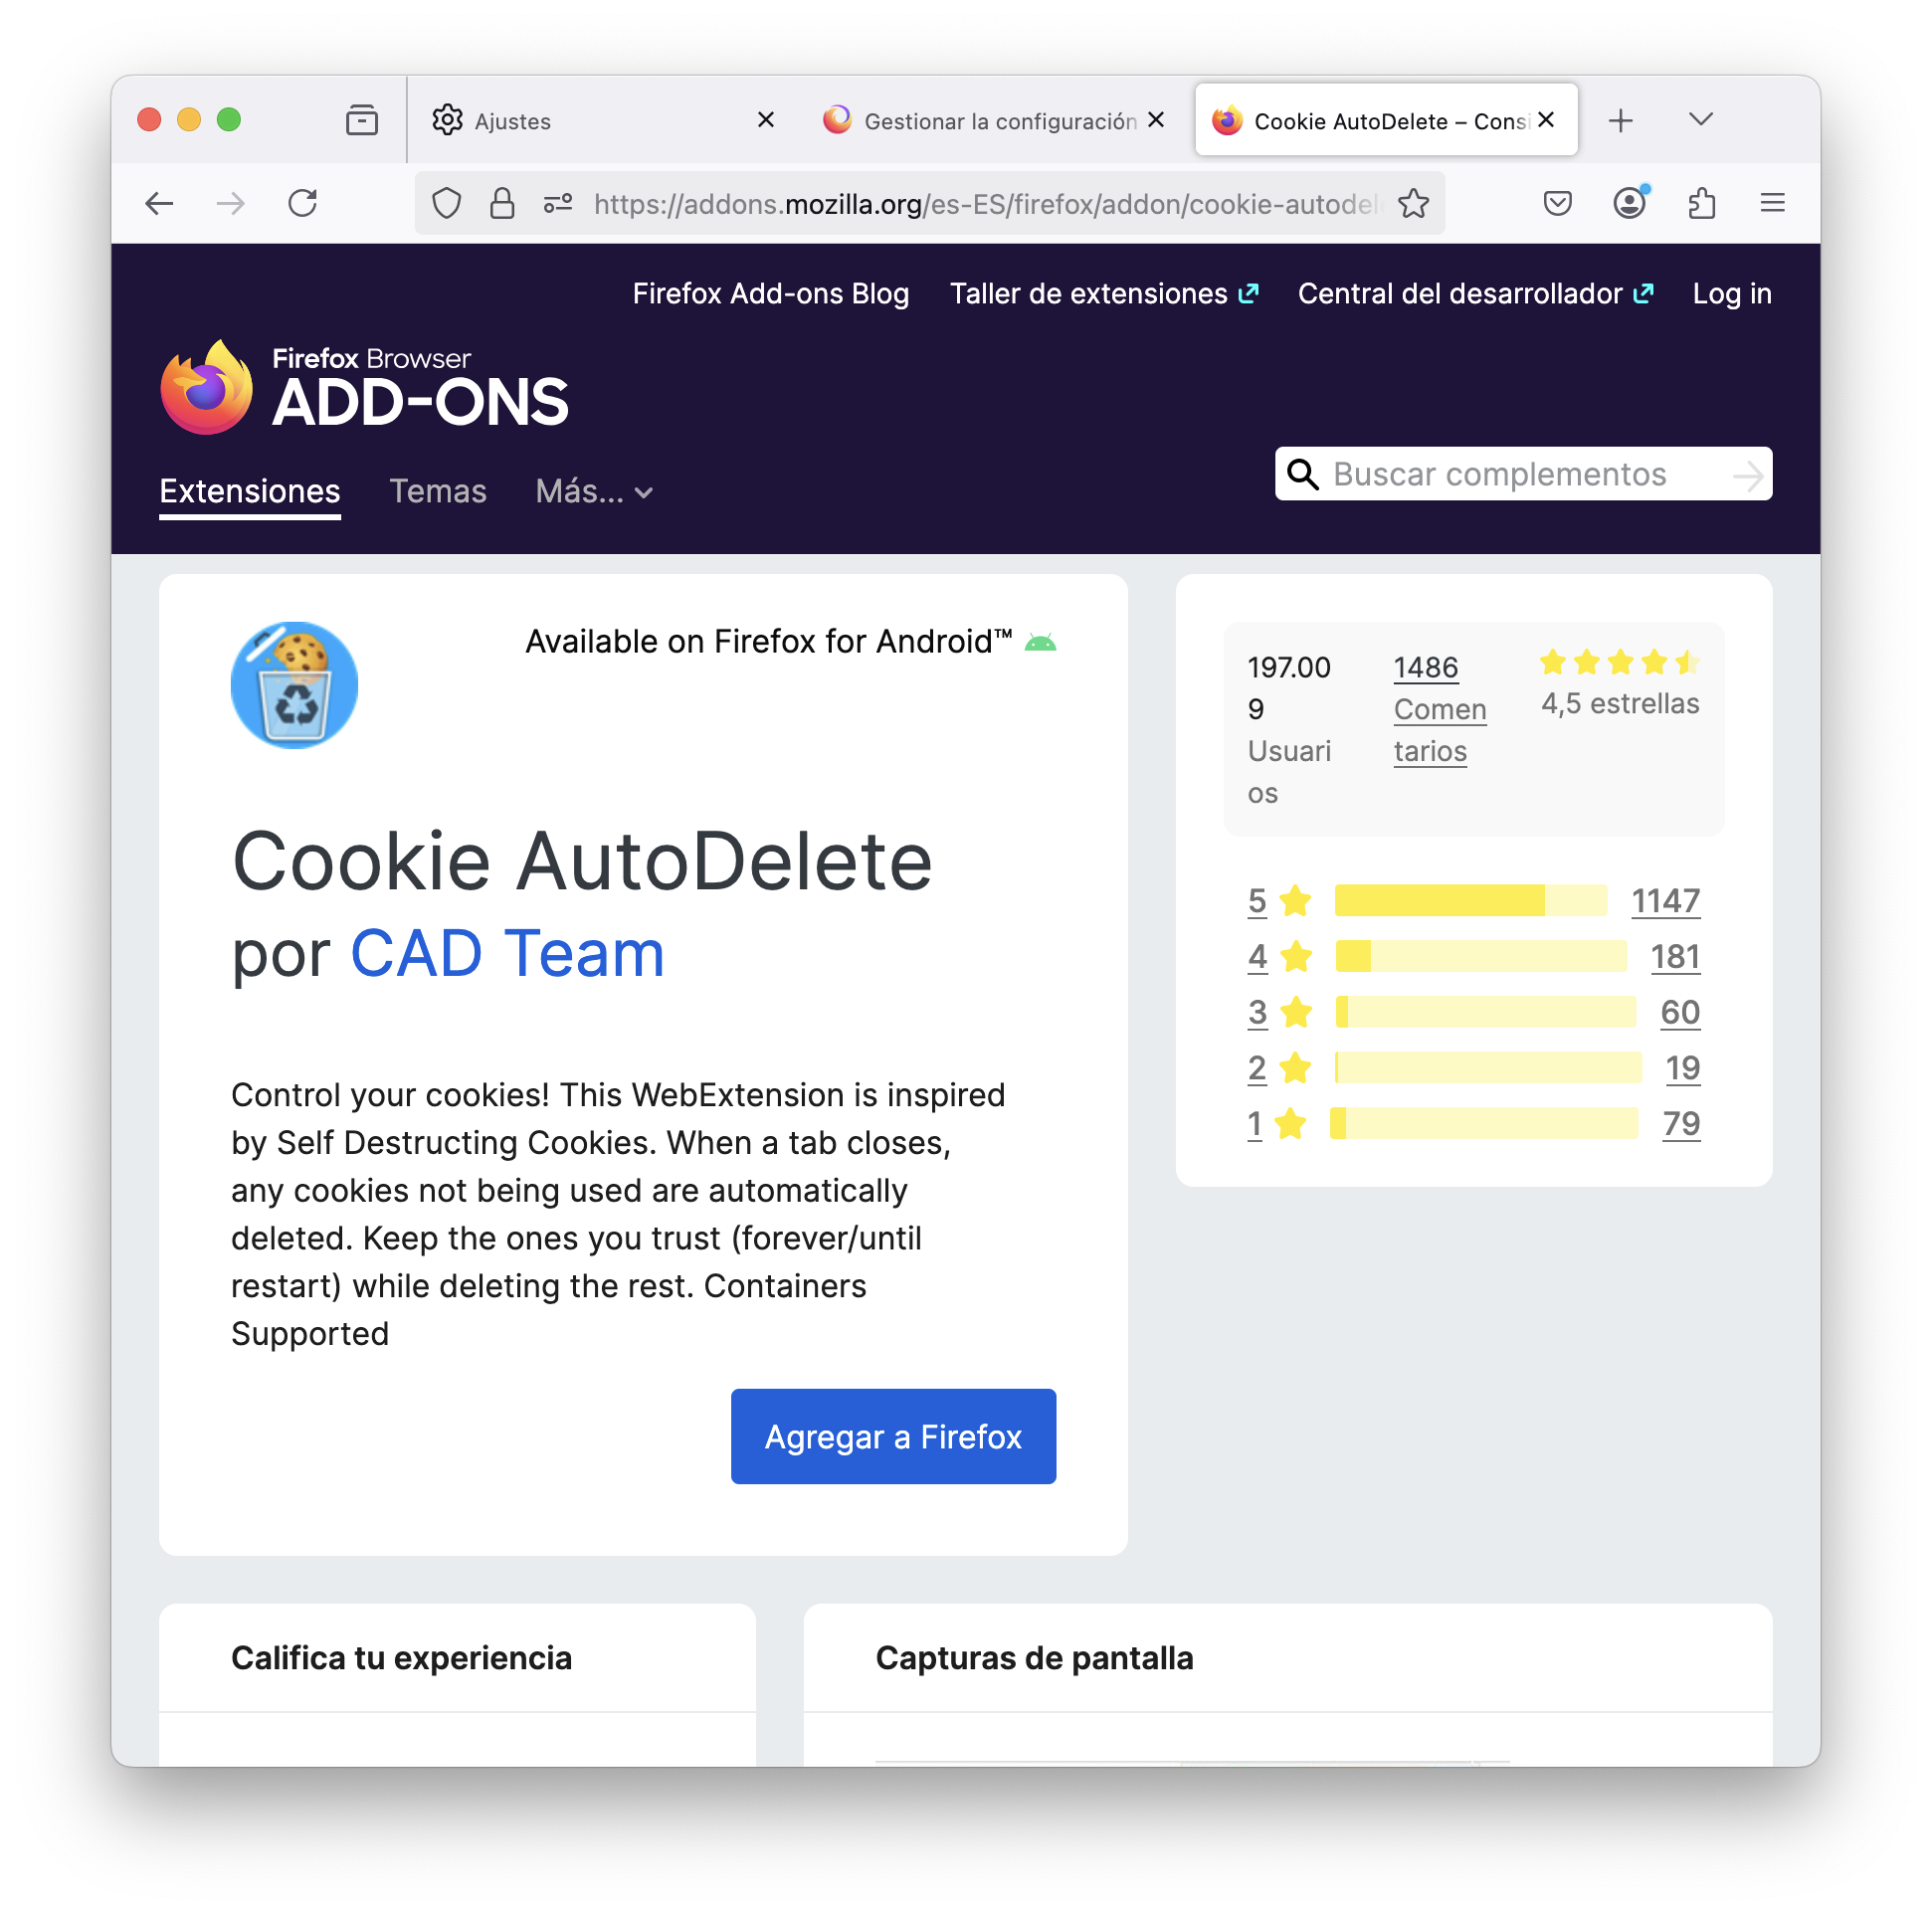
\includegraphics[width=15cm]{addon_cookie_autodelete.png}
    \caption{Add on de cookie Autodelete}
    \label{fig:addon_cookie_autodelete}
\end{figure}

\begin{figure}[H]   
    
\includegraphics[width=15cm]{addon_privacybadger.png}
    \caption{Add on de Privacy Badger}
    \label{fig:addon_privacybadger}
\end{figure}

\begin{figure}[H]   
    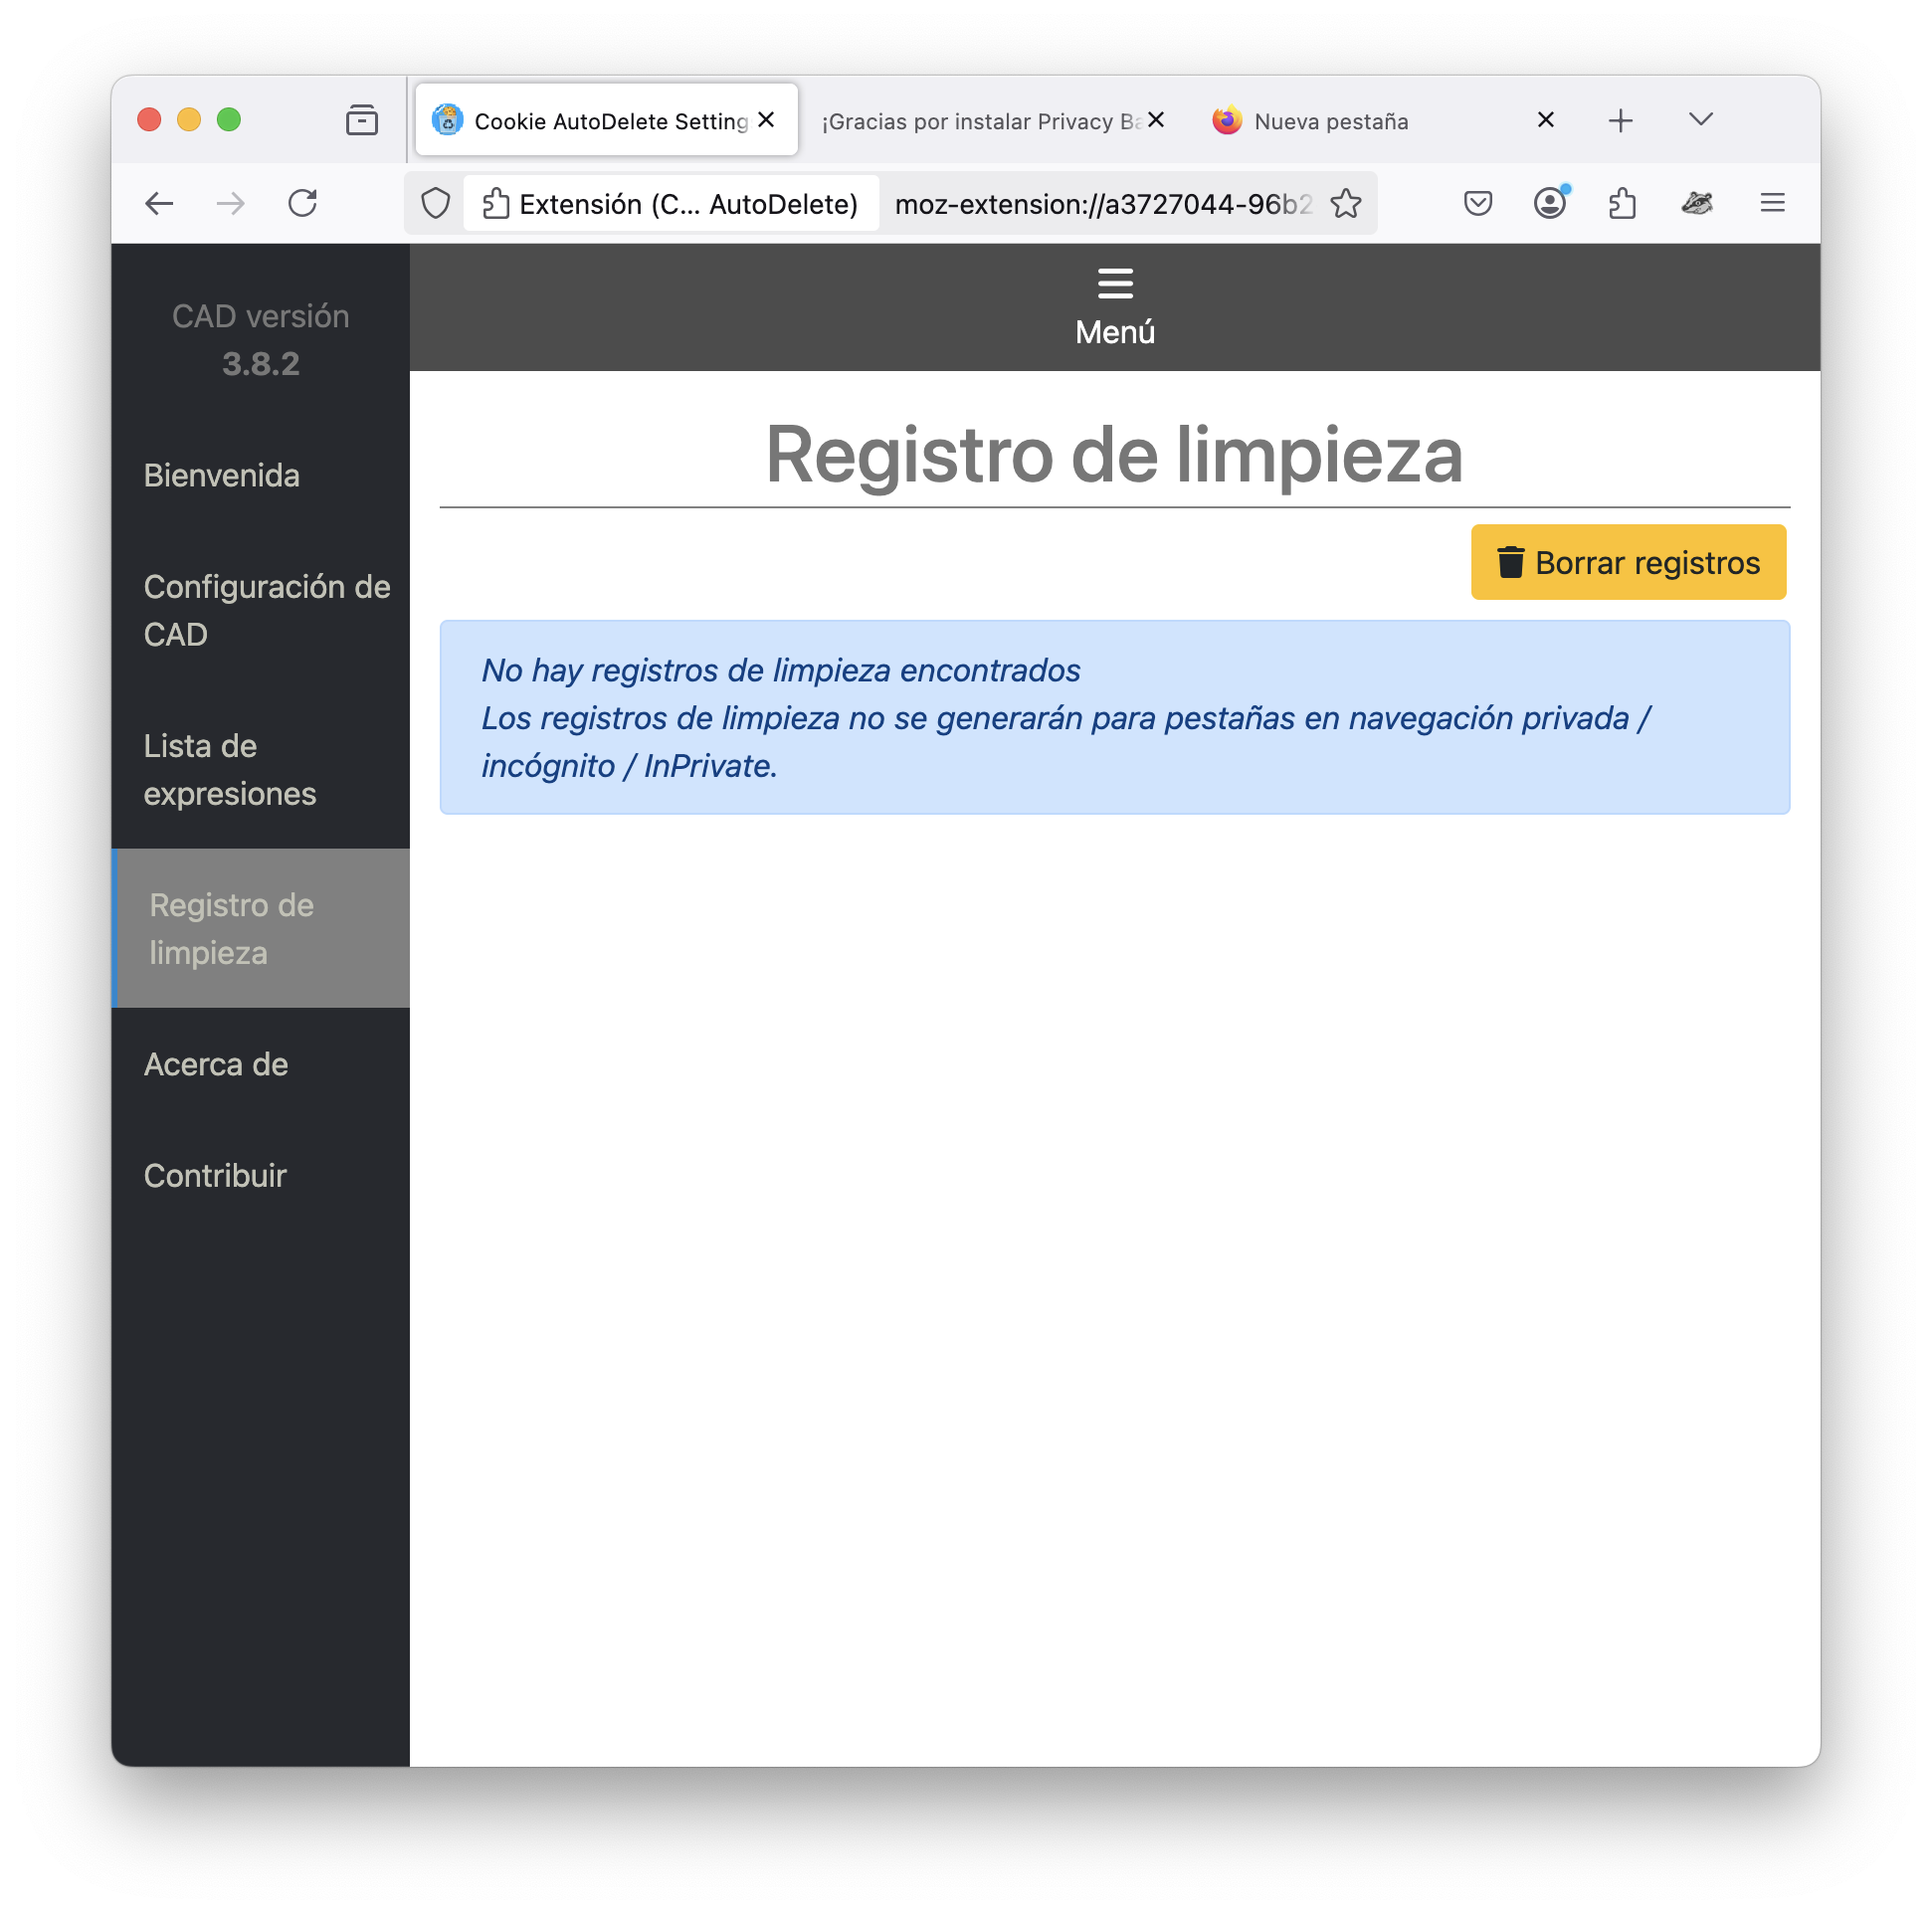
\includegraphics[width=15cm]{activacion_cookie_autodelete.png}
    \caption{Activacion Cookie Autodelete}
    \label{fig:activacion_cookie_autodelete}
\end{figure}

\begin{figure}[H]   
    \includegraphics[width=15cm]{cookies_lavoz.png}
    \caption{Cookies la Voz de Galicia}
    \label{fig:cookies_lavoz}
\end{figure}

\begin{figure}[H]   
    \includegraphics[width=15cm]{resultado_cookies_autodelete.png}
    \caption{Resultado Cookies Autodelete}
    \label{fig:resultado_cookies_autodelete}
\end{figure}

\begin{figure}[H]   
    \includegraphics[width=15cm]{resultado_privacybadger.png}
    \caption{Resultado Privacy Badger}
    \label{fig:resultado_privacybadger}
\end{figure}
\subsection{Ejercicio 15}
\graphicspath{ {img/15} }

\paragraph{Apartado a)} Dentro de las opciones disponibles en el plan gratuito de ProtonVPN podemos destacar \textbf{Quick connect}, que nos permite conectarnos a una VPN escogida automáticamente, en vez de seleccionar manualmente el país/servidor al que conectarnos (en este plan solamente tendremos disponibles conexiones a Japón, Holanda, Polonia, Rumanía y Estados Unidos). Además, contamos con algunas opciones extra en el apartado \texttt{Settings}, como por ejemplo:

\begin{tcolorbox}[
    colback=orange!5!white,
    colframe=orange!75!black,
    title=Opciones relevantes en ProtonVPN
]
\begin{itemize}
    \item \textbf{Kill Switch:} Nos desconecta automáticamente si perdemos la conexión a la VPN.
    \item \textbf{Protocol:} Nos permite cambiar el protocolo de conexión. Podemos elegir entre WireGuard o las dos opciones de OpenVPN: TCP o UDP.
    \item \textbf{IPv6:} Permite filtrar el tráfico que utilice IPv6 a través de la VPN, lo cual aumenta la compatibilidad con redes que utilicen este protocolo.
    \item \textbf{Otras opciones:} También contamos con una opción de cambio de plan además de opciones sobre la aplicación en local, como el iniciarla minimizada o seleccionar nuestras conexiones preferidas como prioritarias.
\end{itemize}
\end{tcolorbox}


\paragraph{Apartado b)} Antes de activar ProtonVPN, miramos las direcciones públicas y privadas de nuestra máquina, además de comprobar nuestra calidad de conexión con el CESGA, mediante RedIRIS.

Como podemos ver en la figura \ref{fig:IPs}, en un principio nuestra IP privada es \\\texttt{192.168.1.141} y la pública \texttt{93.156.217.17}.
Además, nuestra conexión con el CESGA es de \SI{10}{ms} de ping, \SI{2.82}{ms} de jitter, \SI{292}{Mbps} de descarga y \SI{210}{Mbps} de subida.

Estos parámetros son normales dada la distancia que tenemos con el CESGA y que nos estamos conectando directamente.

\begin{figure}[H]
    \centering
    \begin{subfigure}{.5\textwidth}
        \centering
        \includegraphics[width=\linewidth]{IP-Privada.png}
        \caption{Dirección IP Privada}
    \end{subfigure}%
    \begin{subfigure}{.5\textwidth}
        \centering
        \includegraphics[width=\linewidth]{IP-Publica.png}
        \caption{Dirección IP Pública}
    \end{subfigure}
    \caption{Direcciones IP sin ProtonVPN}
    \label{fig:IPs}
\end{figure}


\begin{figure}[H]
    \centering
    \includegraphics[width=\linewidth]{CalidadConexion.png}
    \caption{Calidad de la conexión sin ProtonVPN}
    \label{fig:Calidad-Conexión}
\end{figure}


Ahora, activamos ProtonVPN con Quick Connect, por ejemplo. En nuestro caso nos conectó a un servidor de Holanda.

En la figura \ref{fig:IPs-Holanda} podemos ver el resultado. Se observa que han aparecido dos interfaces de red nuevas, una para IPv4 y otra para IPv6, respectivamente. Esto seguramente sea debido a que activamos la opción IPv6 en los ajustes de ProtonVPN.

En cuanto a las direcciones IP, nuestra dirección privada a utilizar será \texttt{10.98.0.40}, mientras que la pública ha cambiado a \texttt{185.177.126.134}.

Si comprobamos nuestra calidad de red como en la figura \ref{fig:Calidad-Conexión-Holanda} vemos que han aumentado el ping y el jitter, mientras que las velocidades de subida y descarga han disminuído, como es de esperar.

\begin{figure}[H]
    \centering
    \begin{subfigure}{.5\textwidth}
        \centering
        \includegraphics[width=\linewidth]{IP-Privada-Holanda.png}
        \caption{Dirección IP Privada}
    \end{subfigure}%
    \begin{subfigure}{.5\textwidth}
        \centering
        \includegraphics[width=\linewidth]{IP-Publica-Holanda.png}
        \caption{Dirección IP Pública}
    \end{subfigure}
    \caption{Direcciones IP desde Holanda}
    \label{fig:IPs-Holanda}
\end{figure}

\begin{figure}[H]
    \centering
    \includegraphics[width=\linewidth]{CalidadConexion-Holanda.png}
    \caption{Calidad de la conexión desde Holanda}
    \label{fig:Calidad-Conexión-Holanda}
\end{figure}


A continuación repetiremos el proceso otras dos veces más (tres en total) cambiando de servidor. La primera con un servidor en Rumanía y la segunda con un servidor en Japón.
Los resultados se muestran desde la figura \ref{fig:IPs-Rumania} a la figura \ref{fig:Calidad-Conexión-Japon}.

\begin{figure}[H]
    \centering
    \begin{subfigure}{.5\textwidth}
        \centering
        \includegraphics[width=\linewidth]{IP-Privada-Rumania.png}
        \caption{Dirección IP Privada}
    \end{subfigure}%
    \begin{subfigure}{.5\textwidth}
        \centering
        \includegraphics[width=\linewidth]{IP-Publica-Rumania.png}
        \caption{Dirección IP Pública}
    \end{subfigure}
    \caption{Direcciones IP desde Rumania}
    \label{fig:IPs-Rumania}
\end{figure}

\begin{figure}[H]
    \centering
    \includegraphics[width=\linewidth]{CalidadConexion-Rumania.png}
    \caption{Calidad de la conexión desde Rumania}
    \label{fig:Calidad-Conexión-Rumania}
\end{figure}


\begin{figure}[H]
    \centering
    \begin{subfigure}{.5\textwidth}
        \centering
        \includegraphics[width=\linewidth]{IP-Privada-Japon.png}
        \caption{Dirección IP Privada}
    \end{subfigure}%
    \begin{subfigure}{.5\textwidth}
        \centering
        \includegraphics[width=\linewidth]{IP-Publica-Japon.png}
        \caption{Dirección IP Pública}
    \end{subfigure}
    \caption{Direcciones IP desde Japon}
    \label{fig:IPs-Japon}
\end{figure}

\begin{figure}[H]
    \centering
    \includegraphics[width=\linewidth]{CalidadConexion-Japon.png}
    \caption{Calidad de la conexión desde Japon}
    \label{fig:Calidad-Conexión-Japon}
\end{figure}

\subsection{Ejercicio 16}
\graphicspath{ {img/16} }


Antes de realizar el proceso con la VPN de la UDC, comprobamos nuestras direcciones IP privada y pública junto con la calidad de la conexión de la misma manera que en el ejercicio anterior. Mostraremos las características en las figuras \ref{fig:IPs-preUDC} y \ref{fig:Calidad-Conexión-preUDC}.

\begin{figure}[H]
    \centering
    \begin{subfigure}{.5\textwidth}
        \centering
        \includegraphics[width=\linewidth]{IP-Privada-preUDC.png}
        \caption{Dirección IP Privada}
    \end{subfigure}%
    \begin{subfigure}{.5\textwidth}
        \centering
        \includegraphics[width=\linewidth]{IP-Publica-preUDC.png}
        \caption{Dirección IP Pública}
    \end{subfigure}
    \caption{Direcciones IP antes de utilizar la VPN de la UDC}
    \label{fig:IPs-preUDC}
\end{figure}

\begin{figure}[H]
    \centering
    \includegraphics[width=\linewidth]{CalidadConexion-preUDC.png}
    \caption{Calidad de la conexión antes de utilizar la VPN de la UDC}
    \label{fig:Calidad-Conexión-preUDC}
\end{figure}


Observamos que las IPs privada y pública son \texttt{192.168.1.142} (primera interfaz de red) y \texttt{93.156.217.17}, respectivamente, y que contamos con una velocidad de \SI{550}{Mbps} (de descarga) y \SI{440}{Mbps} de carga, además de \SI{16}{ms} de latencia de carga/descarga.

A continuación, para poder utilizar la VPN de la UDC primero debemos instalarla y configurarla en el enlace \href{https://axudatic.udc.gal/pages/viewpage.action?pageId=45813771}{\texttt{VPN-UDC}}, dentro del apartado \texttt{`Instalación e configuración'}.

Con el cliente de VPN instalado, nos conectamos y reexaminamos los parámetros de la conexión, tal y como muestran las figuras \ref{fig:IPs-VPN-UDC} y \ref{fig:Calidad-Conexión-VPN-UDC}.

\begin{figure}[H]
    \centering
    \begin{subfigure}{.5\textwidth}
        \centering
        \includegraphics[width=\linewidth]{IP-Privada-VPN-UDC.png}
        \caption{Dirección IP Privada}
    \end{subfigure}%
    \begin{subfigure}{.5\textwidth}
        \centering
        \includegraphics[width=\linewidth]{IP-Publica-VPN-UDC.png}
        \caption{Dirección IP Pública}
    \end{subfigure}
    \caption{Direcciones IP antes de utilizar la VPN de la UDC}
    \label{fig:IPs-VPN-UDC}
\end{figure}

\begin{figure}[H]
    \centering
    \includegraphics[width=\linewidth]{CalidadConexion-VPN-UDC.png}
    \caption{Calidad de la conexión antes de utilizar la VPN de la UDC}
    \label{fig:Calidad-Conexión-VPN-UDC}
\end{figure}


Como podemos ver, la calidad de la red no cambia demasiado, de hecho en el caso de las capturas mejoran las velocidades de carag y descarga, aunque estos resultados varían al realizarlos varias veces.
Esto concuerda con lo esperado, ya que nos encontramos cerca de la UDC.

Lo que sí llega a cambiar son las interfaces de red. Vemos que se genera una nueva interfaz de red (que lleva el sufijo DNS \texttt{udc.pri}), que corresponde a la actividad de la VPN. Su IP (privada) es \texttt{10.30.8.191/32}.
En cambio, la IP pública no cambia al pasar a utilizar la VPN.

\subsection{Ejercicio 17}



\newpage
\setcitestyle{numbers}
\bibliographystyle{apalike}
\bibliography{refs}

\end{document}
